\section{Angular fits}
\label{app:AngRes}

In this section are reported results of fits on angular observables for all considered (and unblinded) \qsq bins.


\begin{figure}[!htb]
\centering
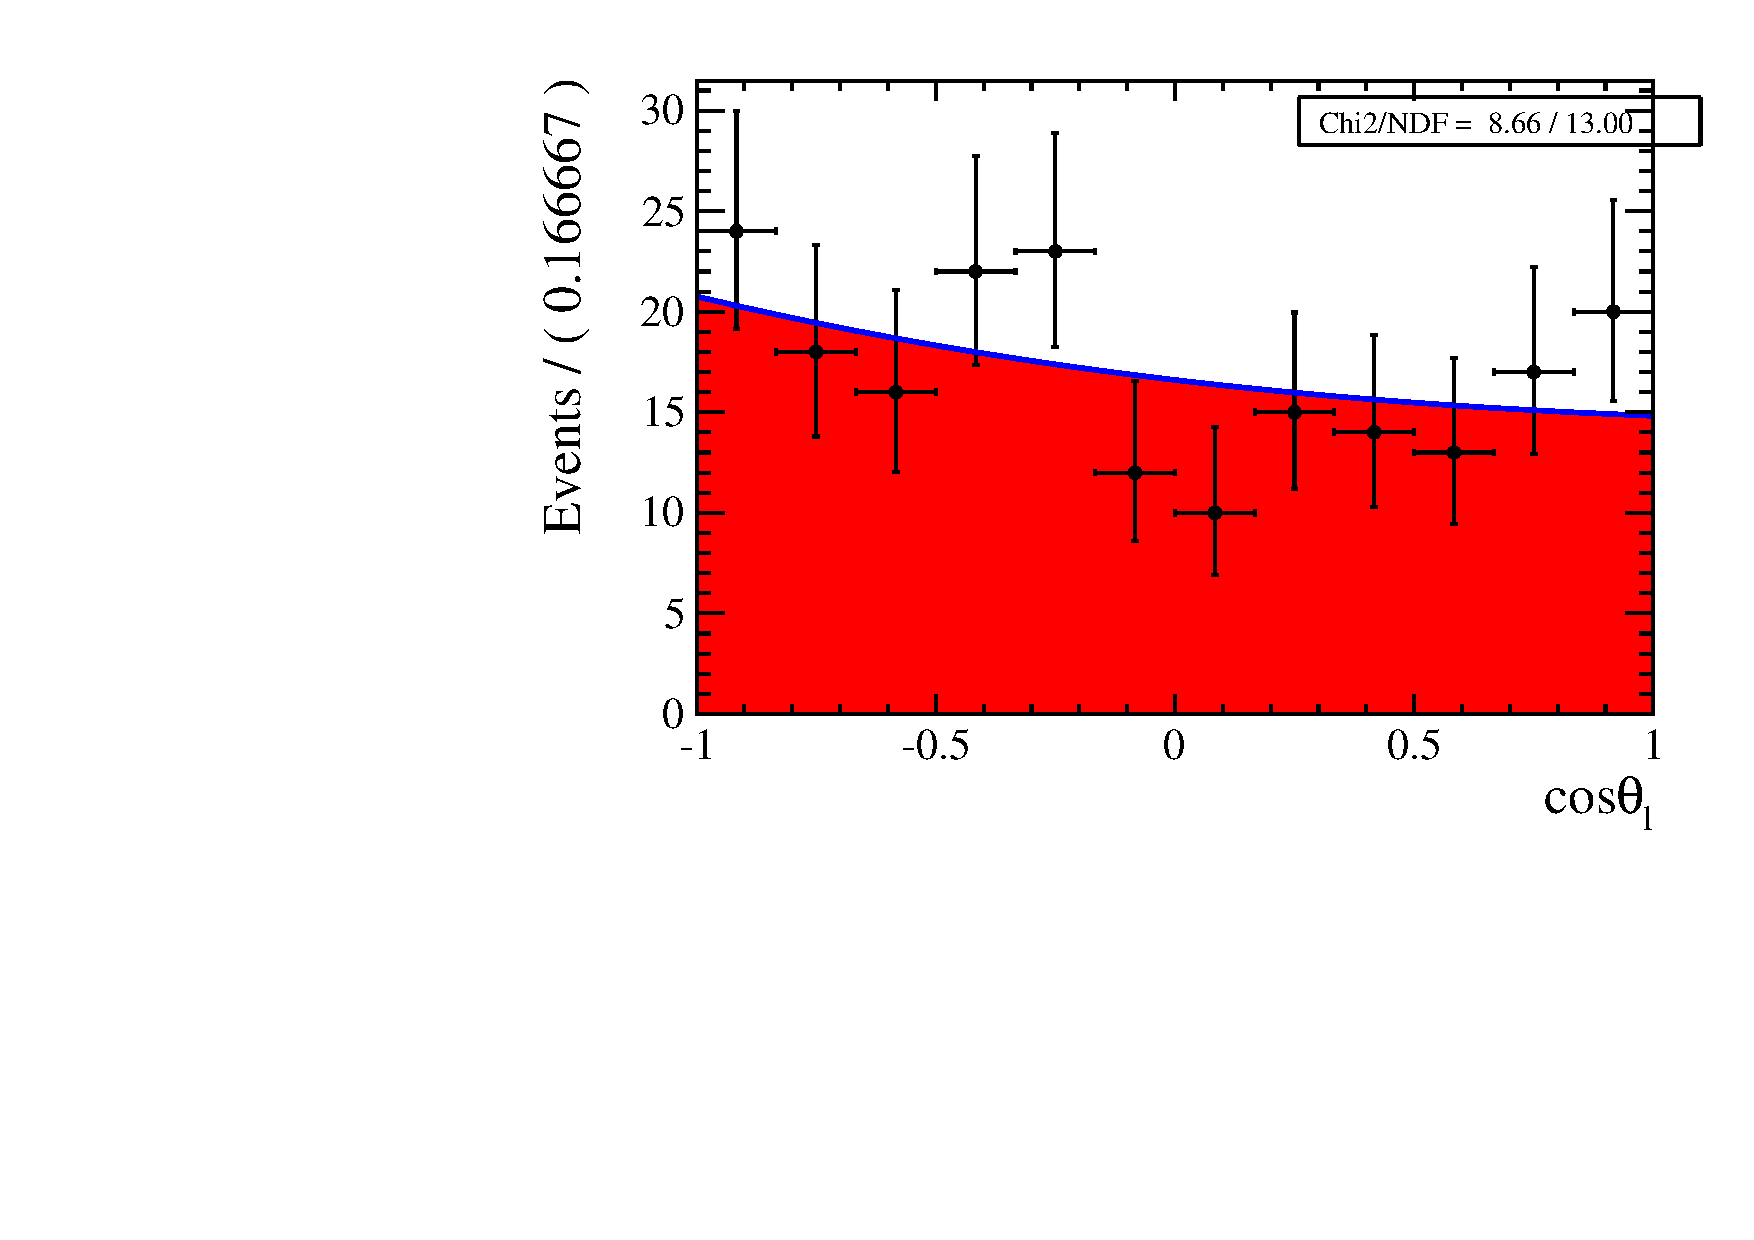
\includegraphics[width=0.40\textwidth]{Lmumu/figs/Side_DD_q2_1500_2000.pdf}
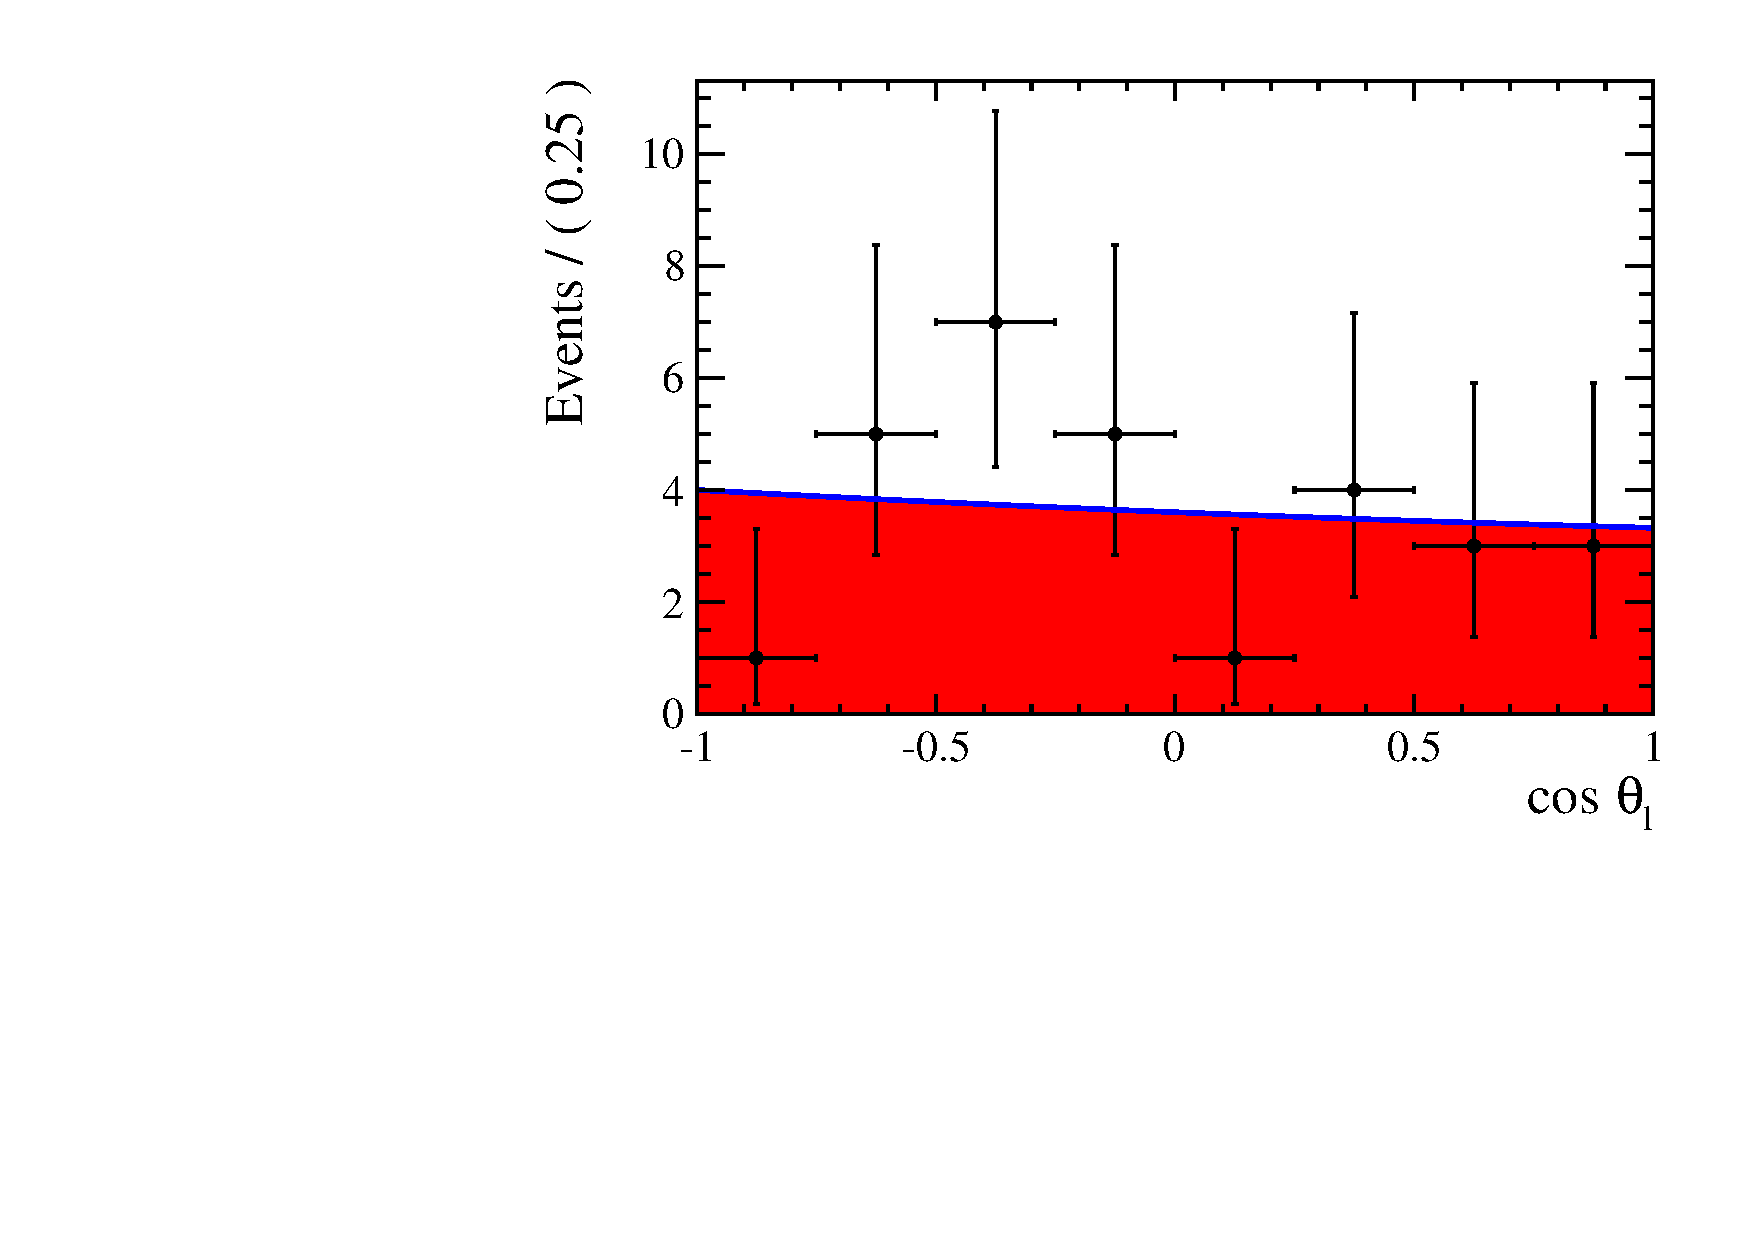
\includegraphics[width=0.40\textwidth]{Lmumu/figs/Side_LL_q2_1500_2000.pdf} \\
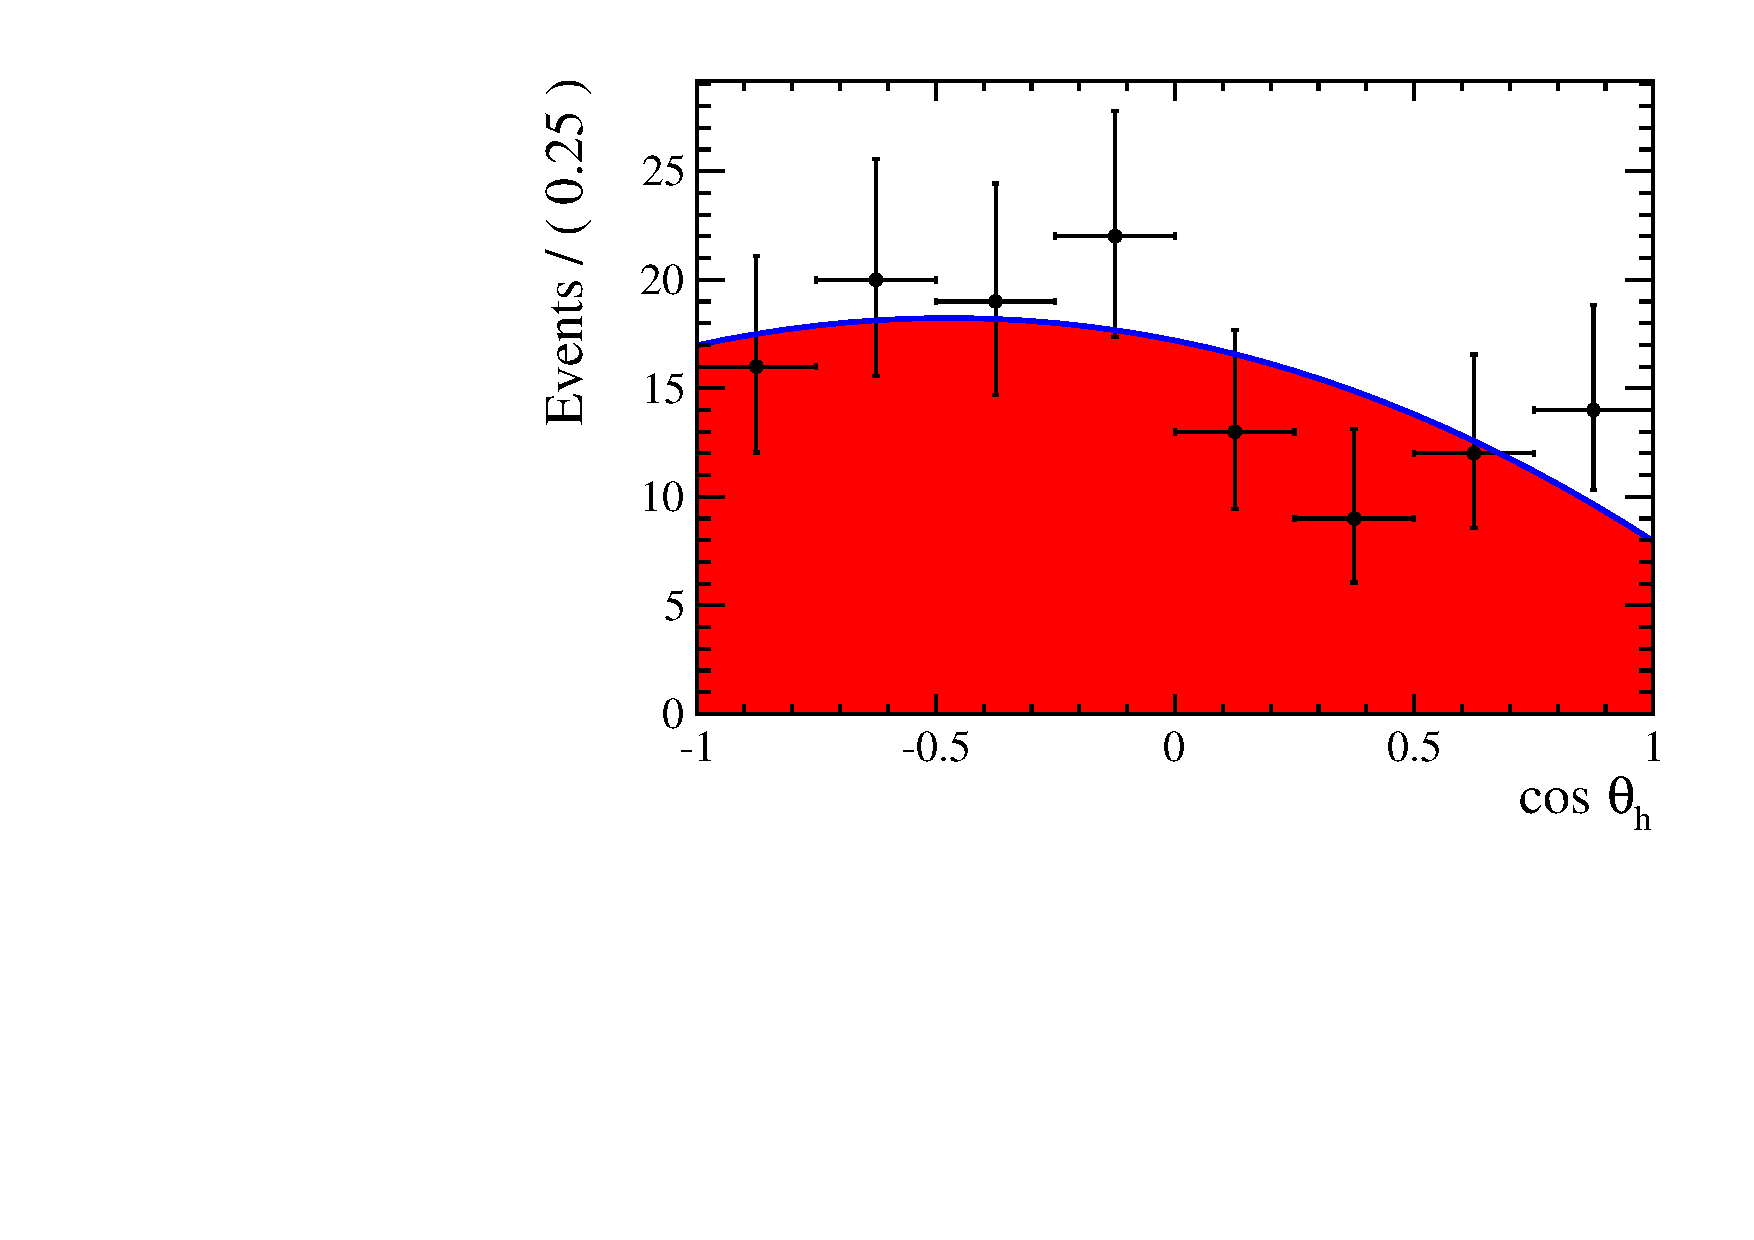
\includegraphics[width=0.40\textwidth]{Lmumu/figs/SideB_DD_q2_1500_2000.pdf}
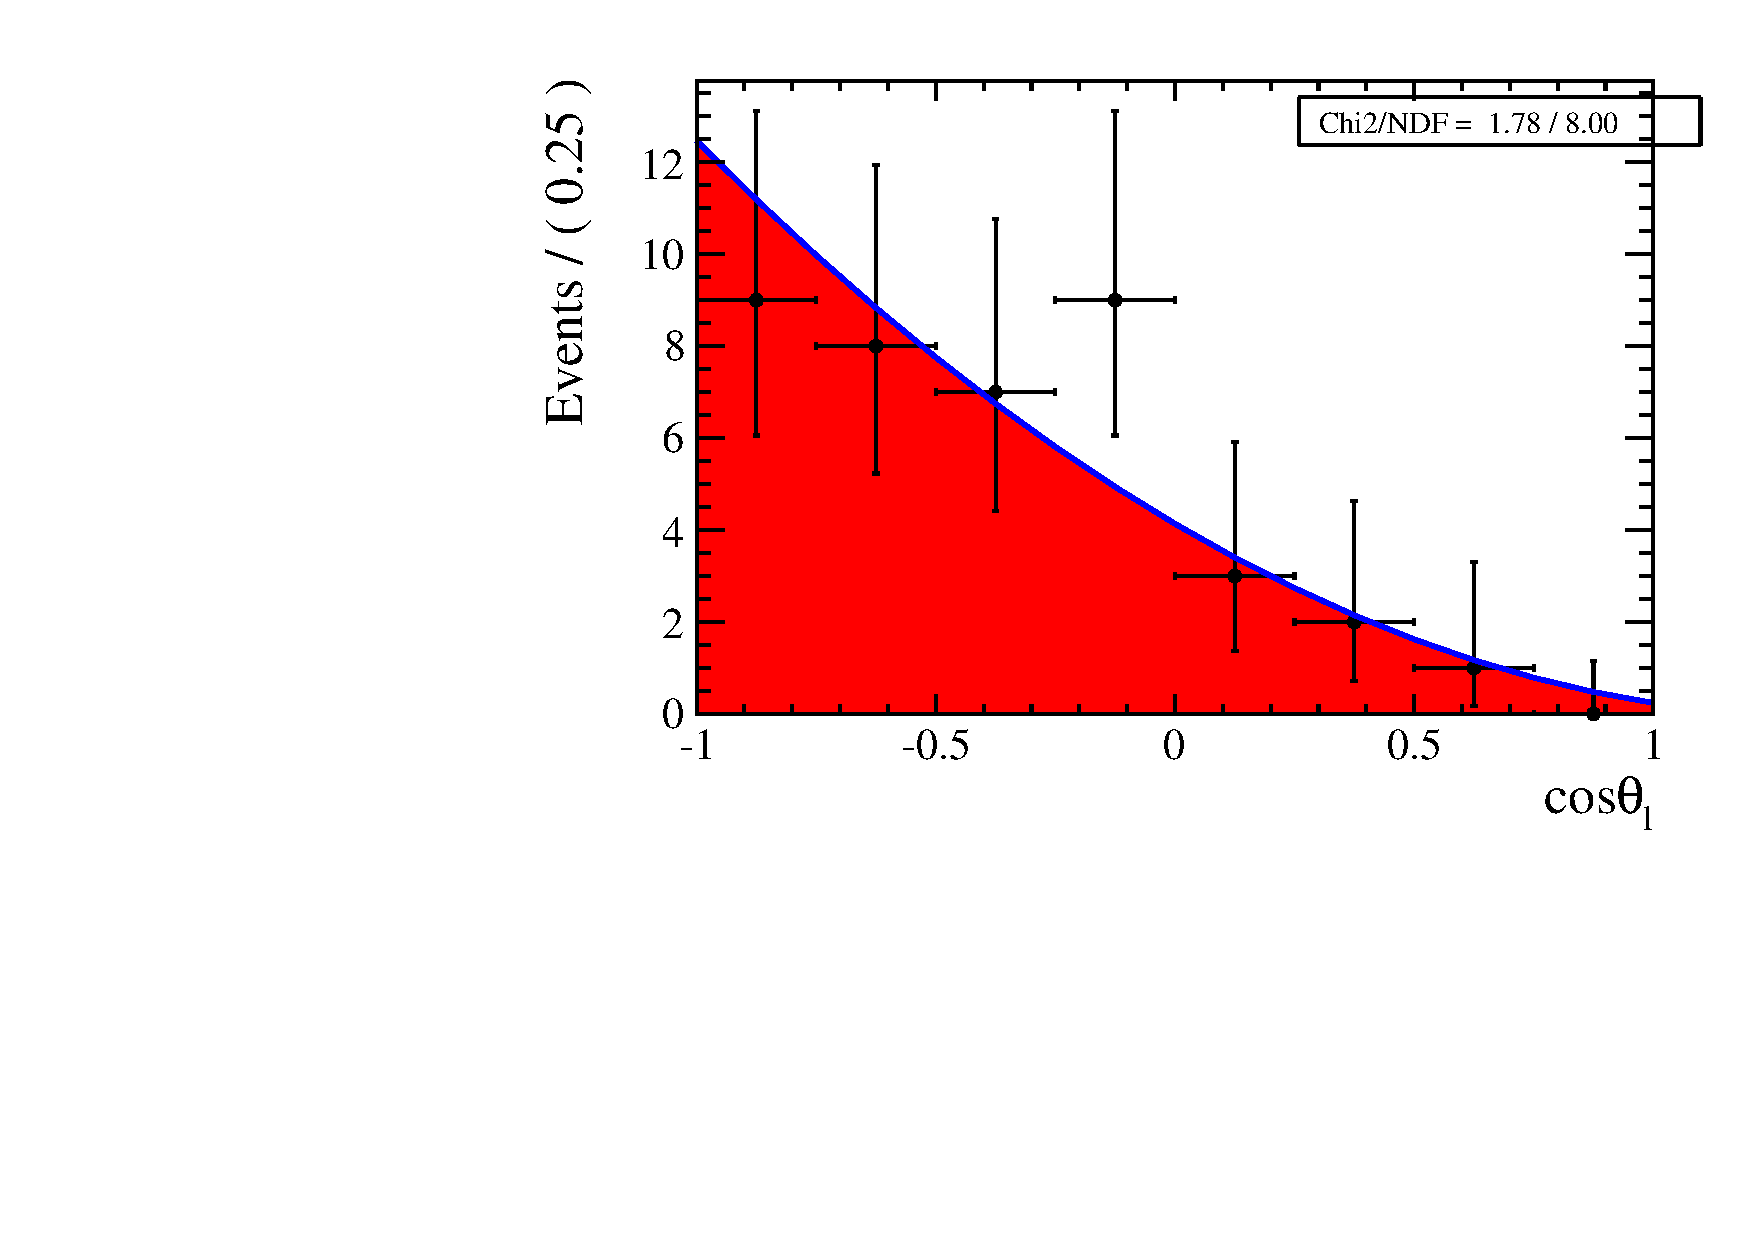
\includegraphics[width=0.40\textwidth]{Lmumu/figs/SideB_LL_q2_1500_2000.pdf}
\caption{Angular distribution in the sideband ($m_{\Lambda\mumu} > 5700 \mevcc$) as a function of $\cos\theta_\Lambda$ (top) and $\cos\theta_\Lambda$ (bottom) for down-down (left) and long-long (right) for events in the $15.0-20.0$GeV^2/c^2$$ \qsq bin.  }
\end{figure}





\begin{figure}[!htb]
\centering
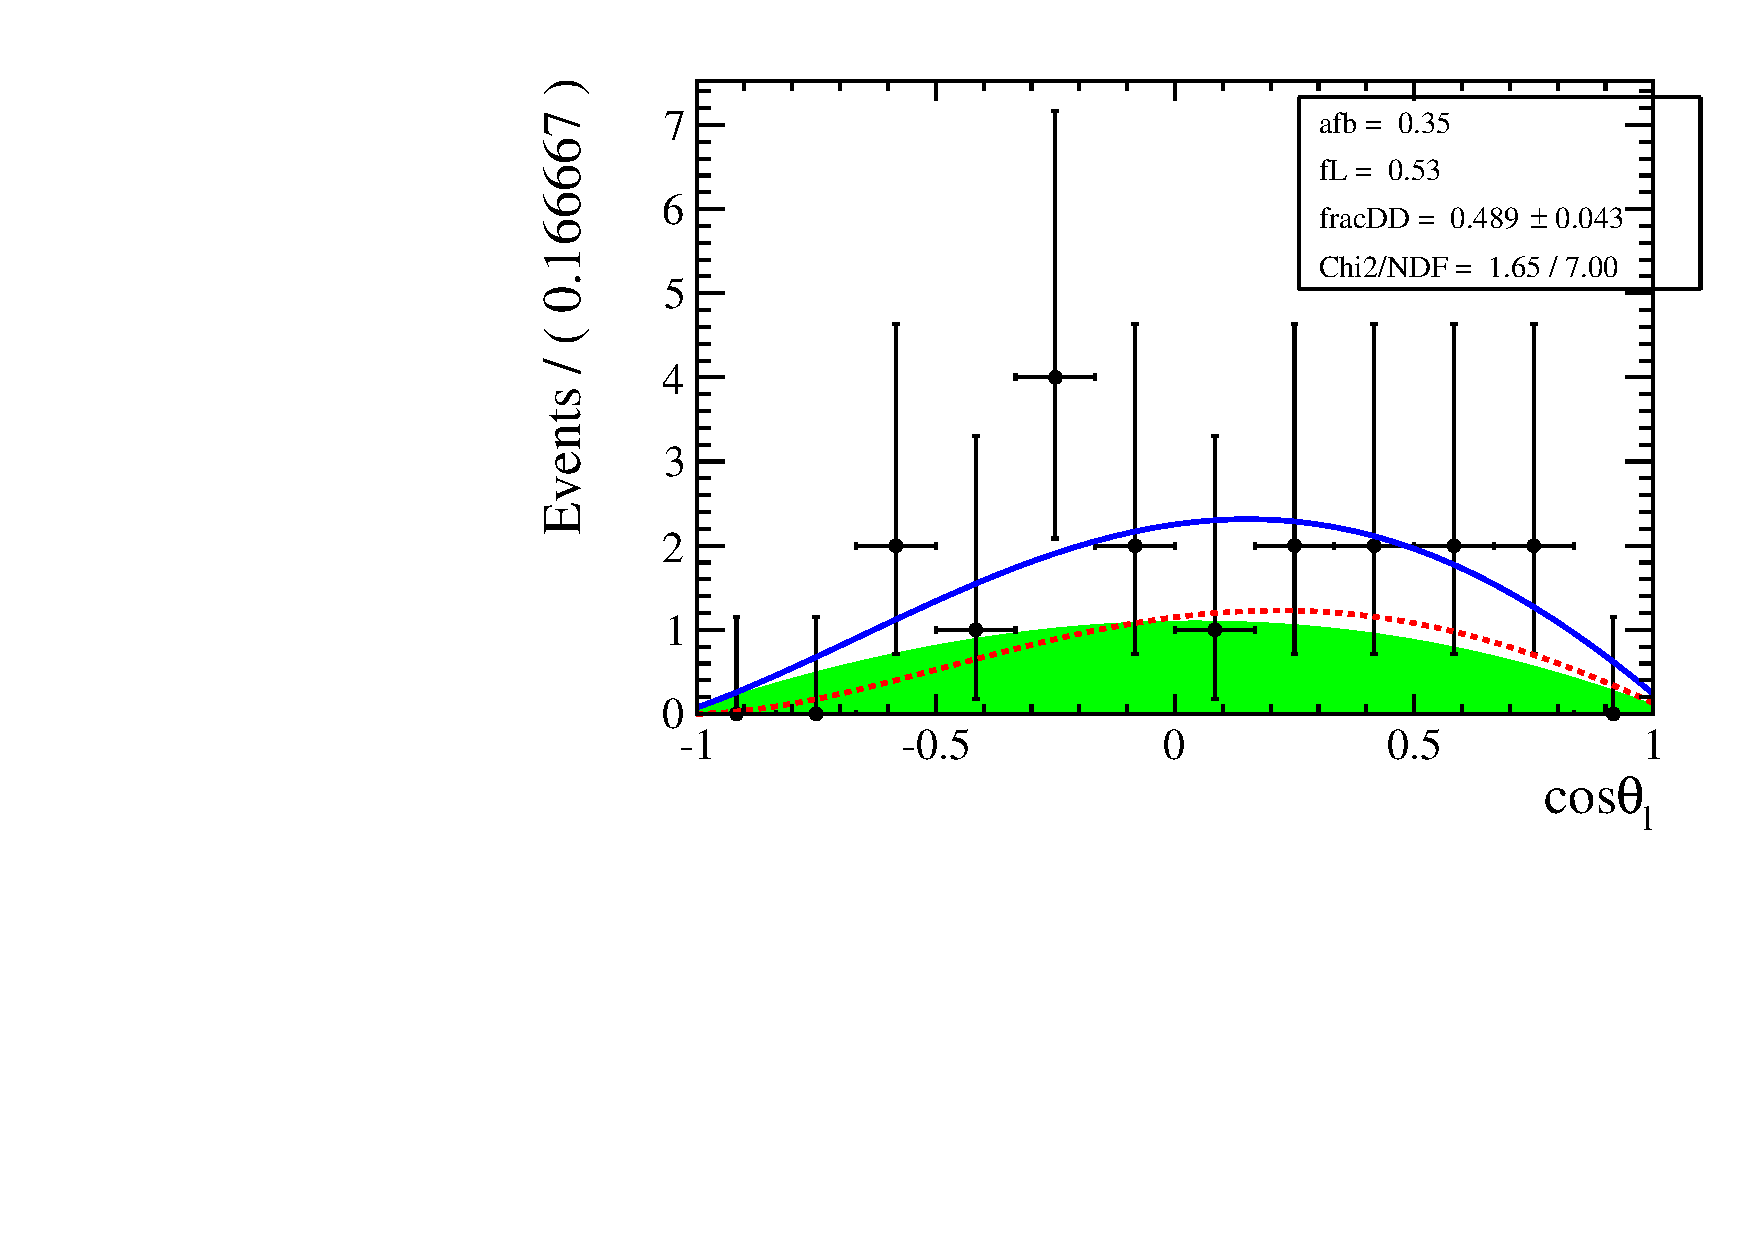
\includegraphics[width=0.40\textwidth]{Lmumu/figs/Afb_DD_q2_010_200.pdf}
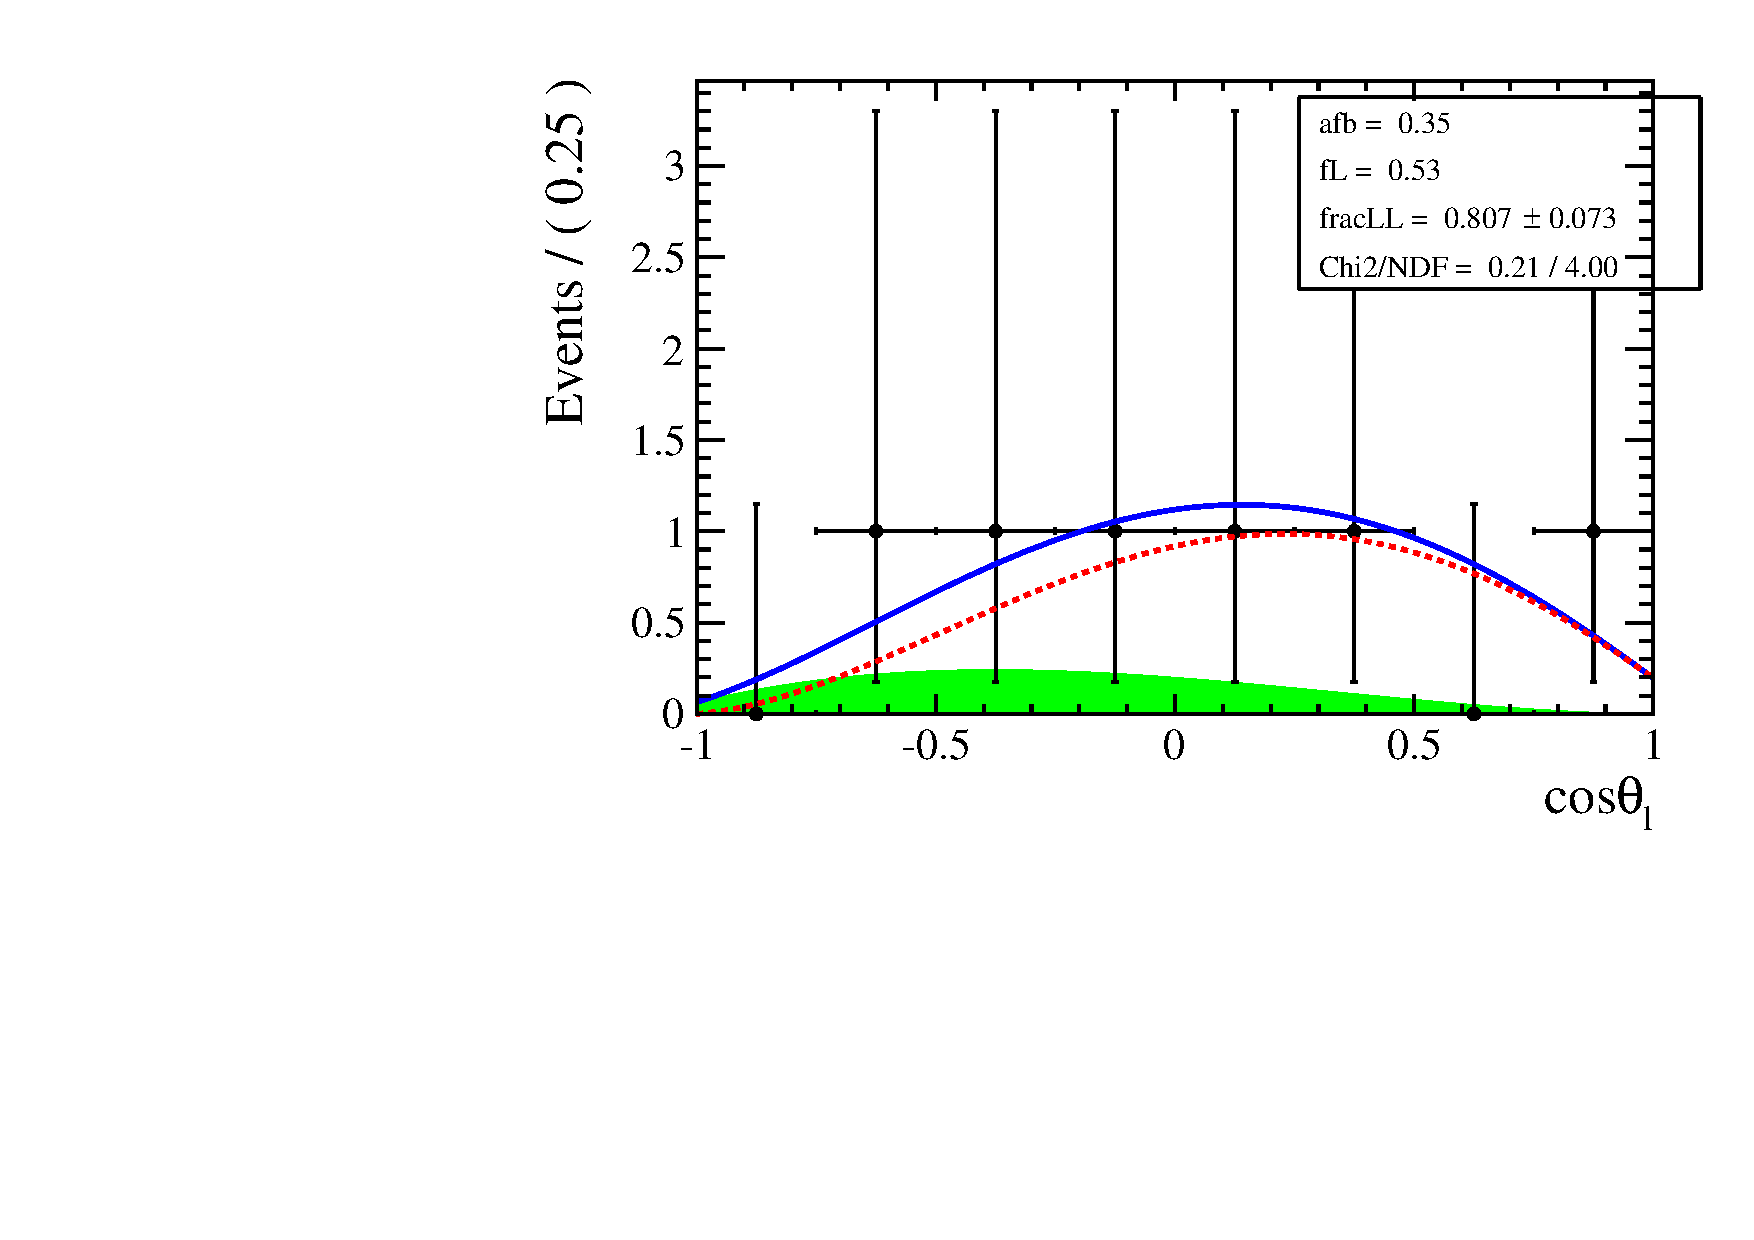
\includegraphics[width=0.40\textwidth]{Lmumu/figs/Afb_LL_q2_010_200.pdf} \\
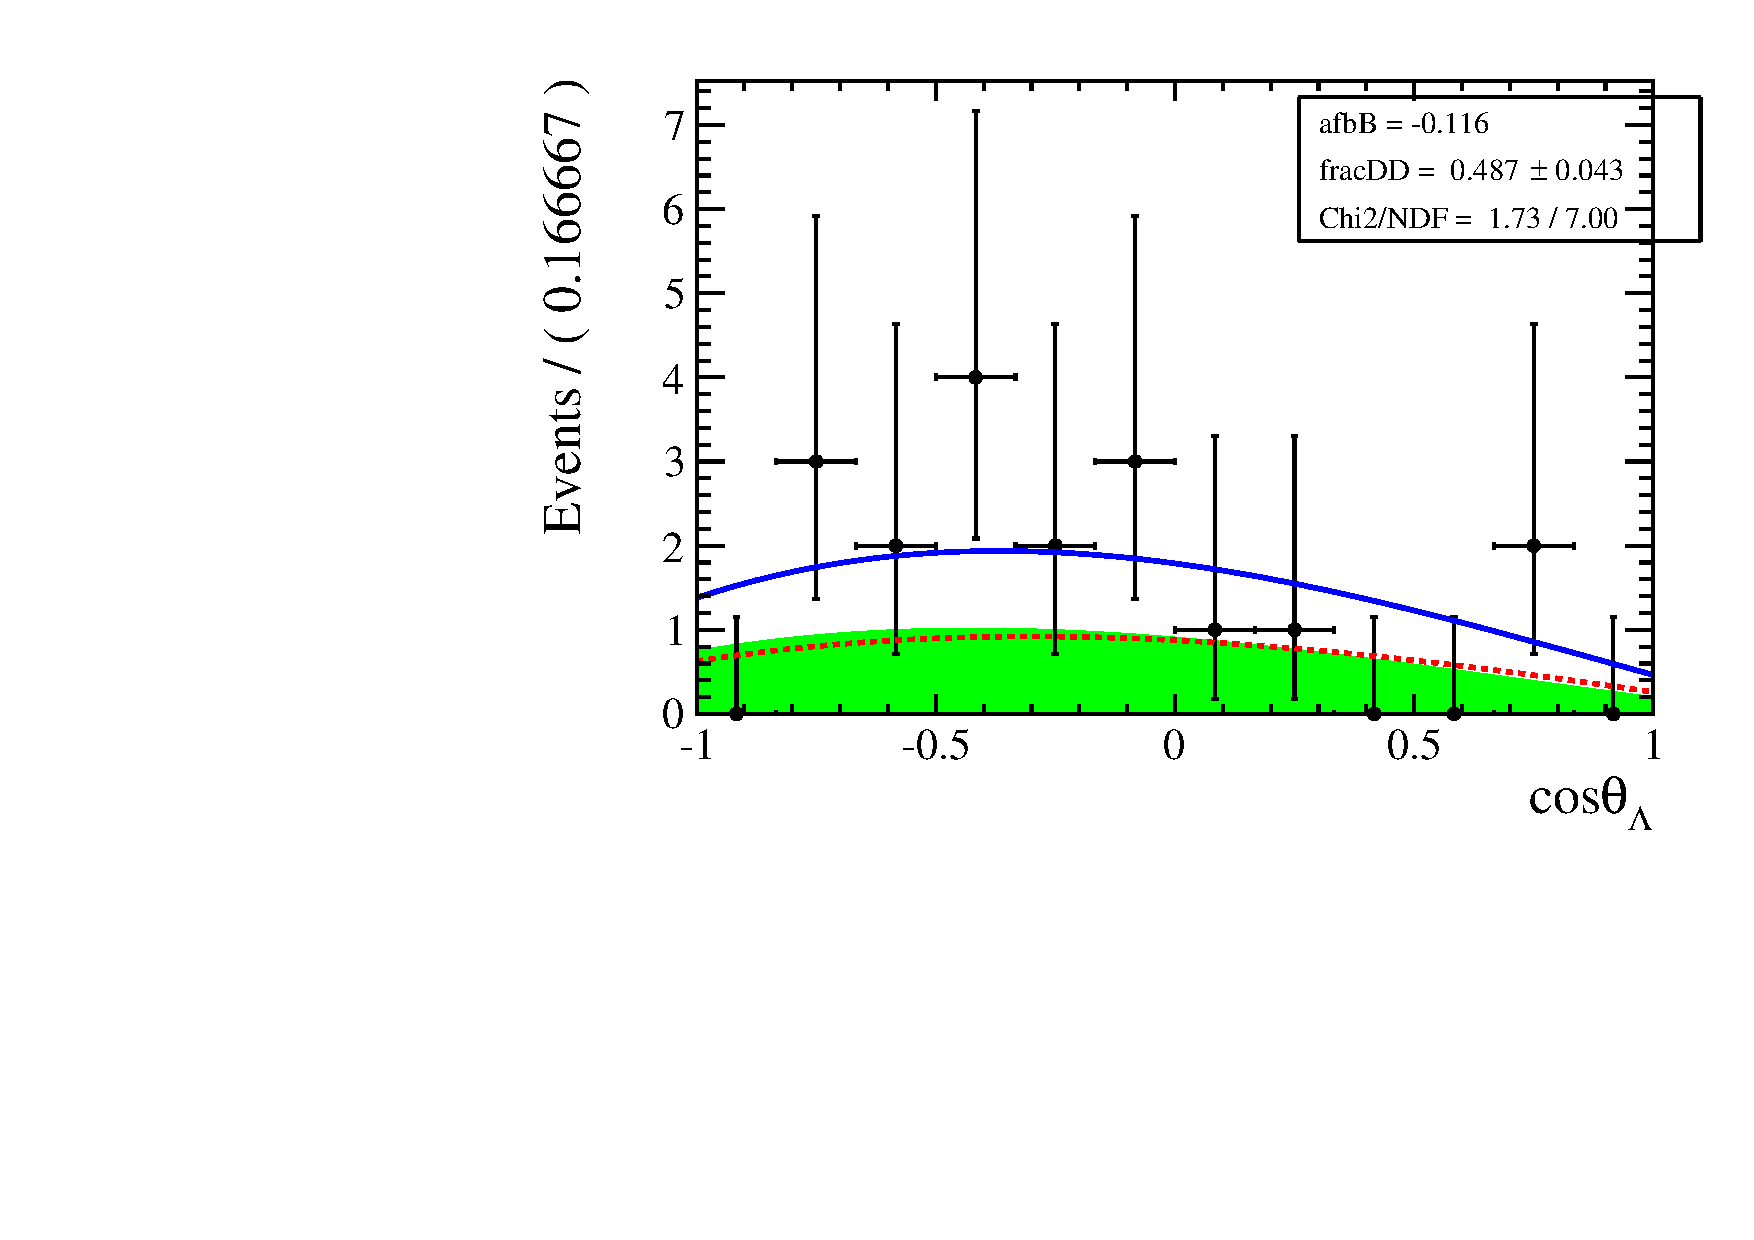
\includegraphics[width=0.40\textwidth]{Lmumu/figs/AfbB_DD_q2_010_200.pdf}
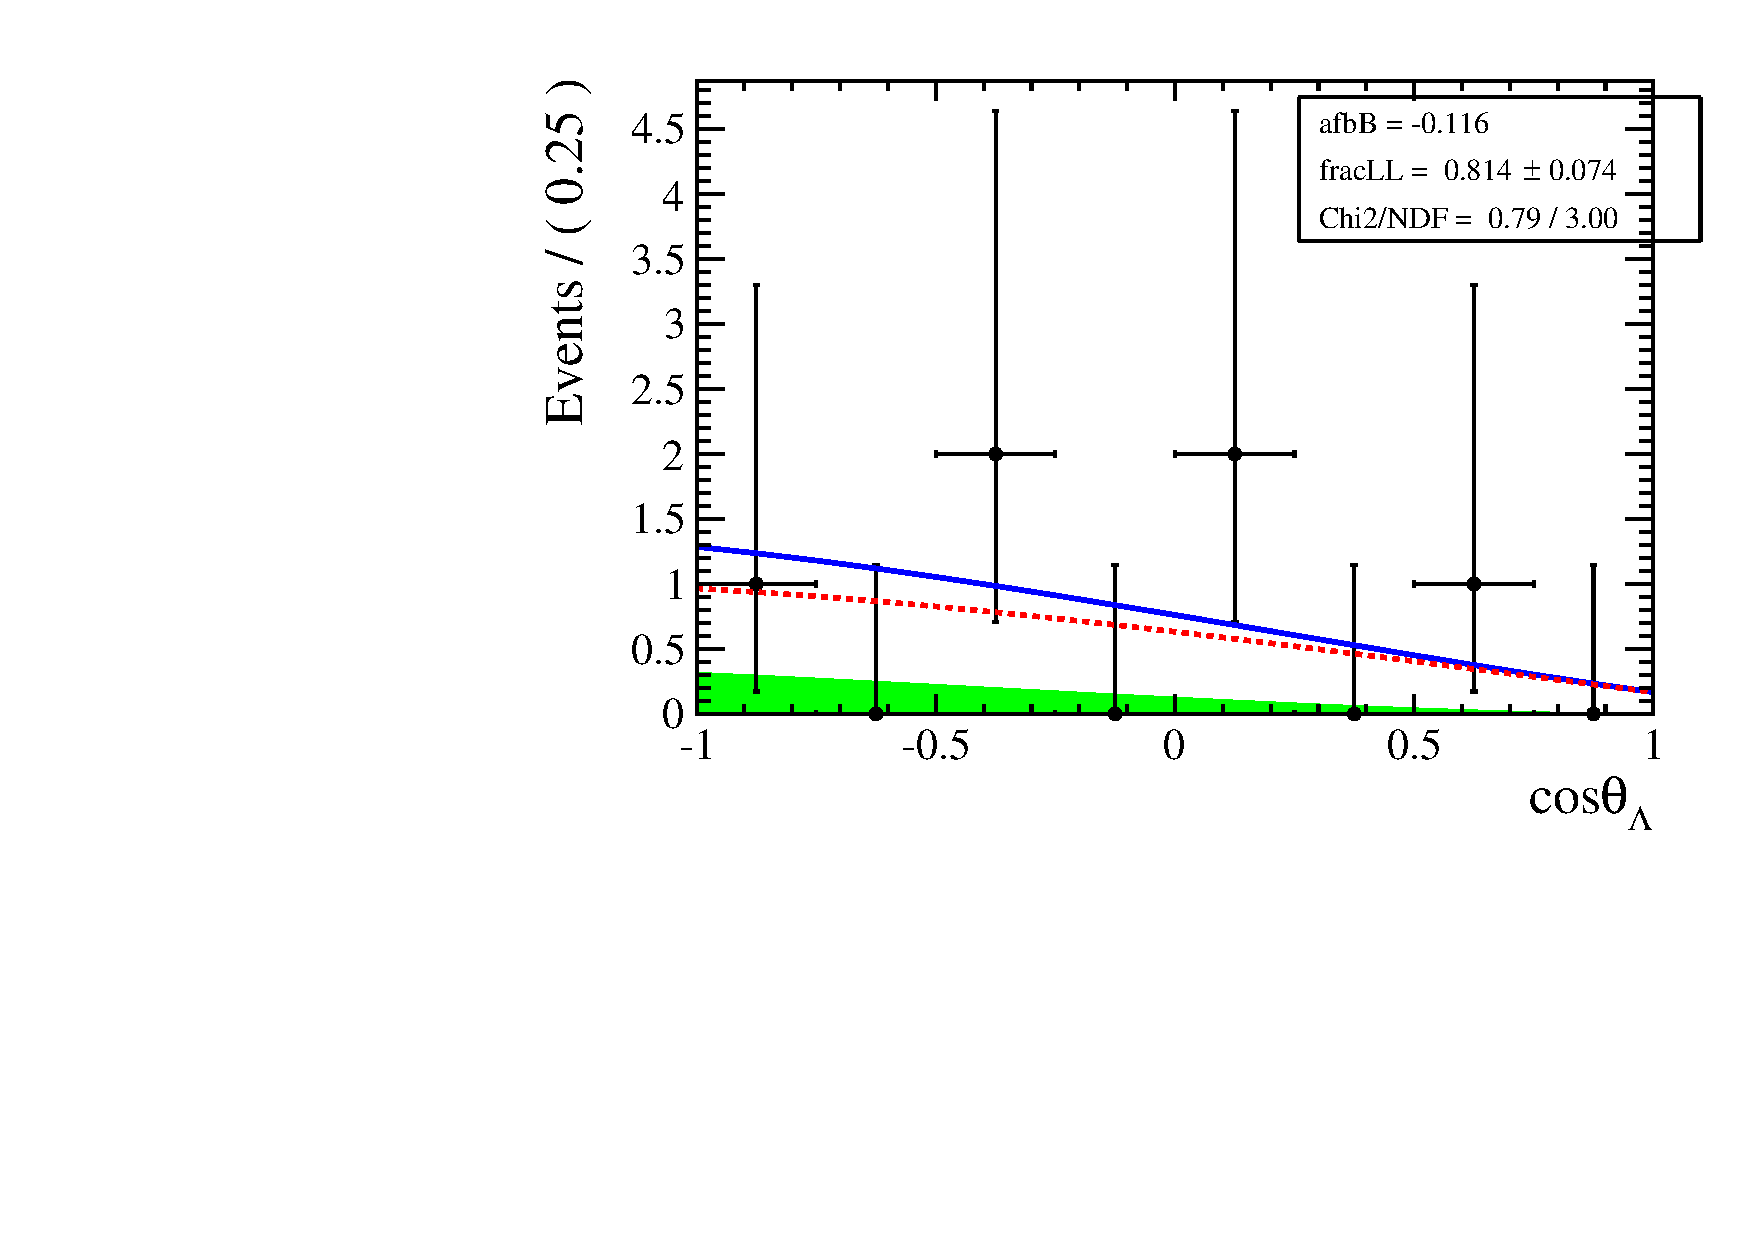
\includegraphics[width=0.40\textwidth]{Lmumu/figs/AfbB_LL_q2_010_200.pdf}
\caption{Fitted angular distribution as a function of $\cos\theta_\ell$ (top) and $\cos\theta_\Lambda$ (bottom) for down-down (left) and long-long (right) events for events in the $0.1-2.0$GeV^2/c^2$$ \qsq bin.  }
\end{figure}


\begin{figure}[!htb]
\centering
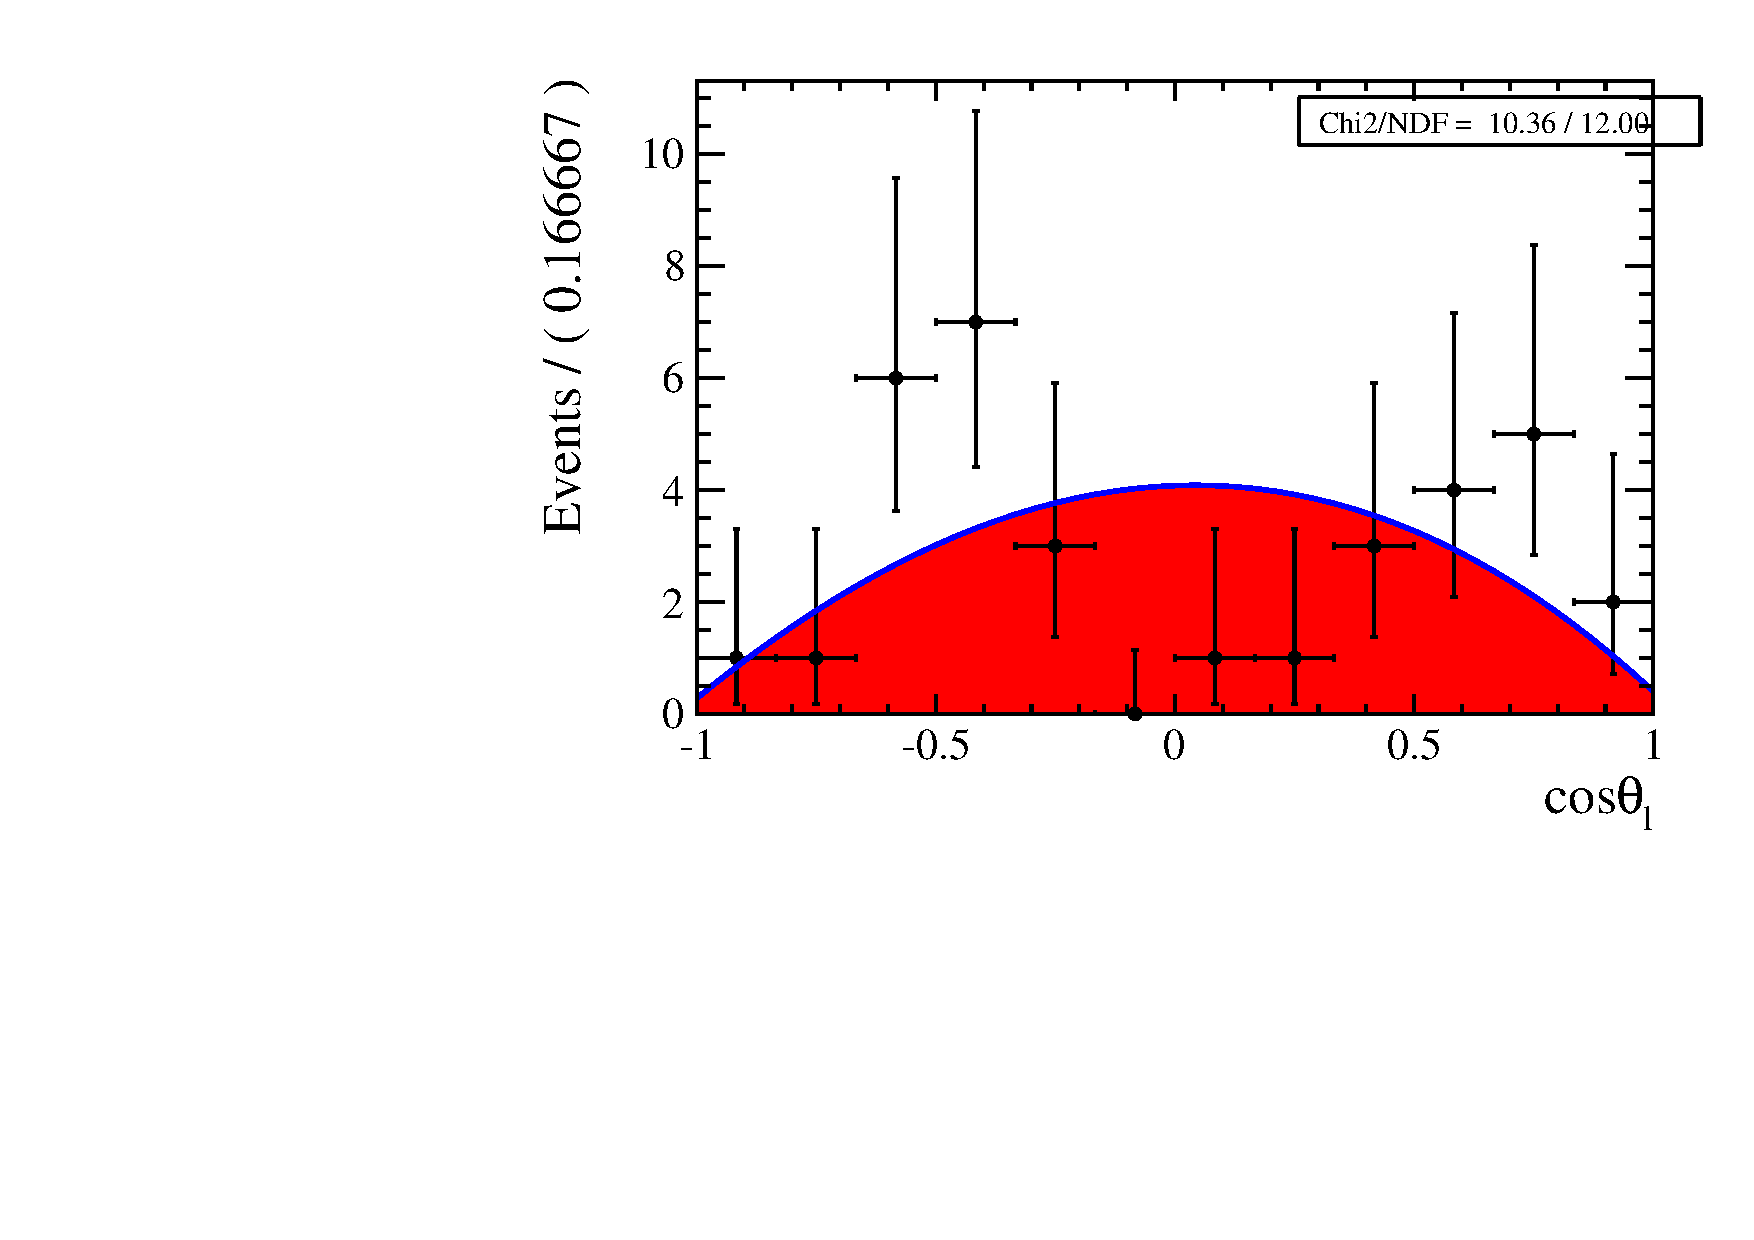
\includegraphics[width=0.40\textwidth]{Lmumu/figs/Side_DD_q2_010_200.pdf}
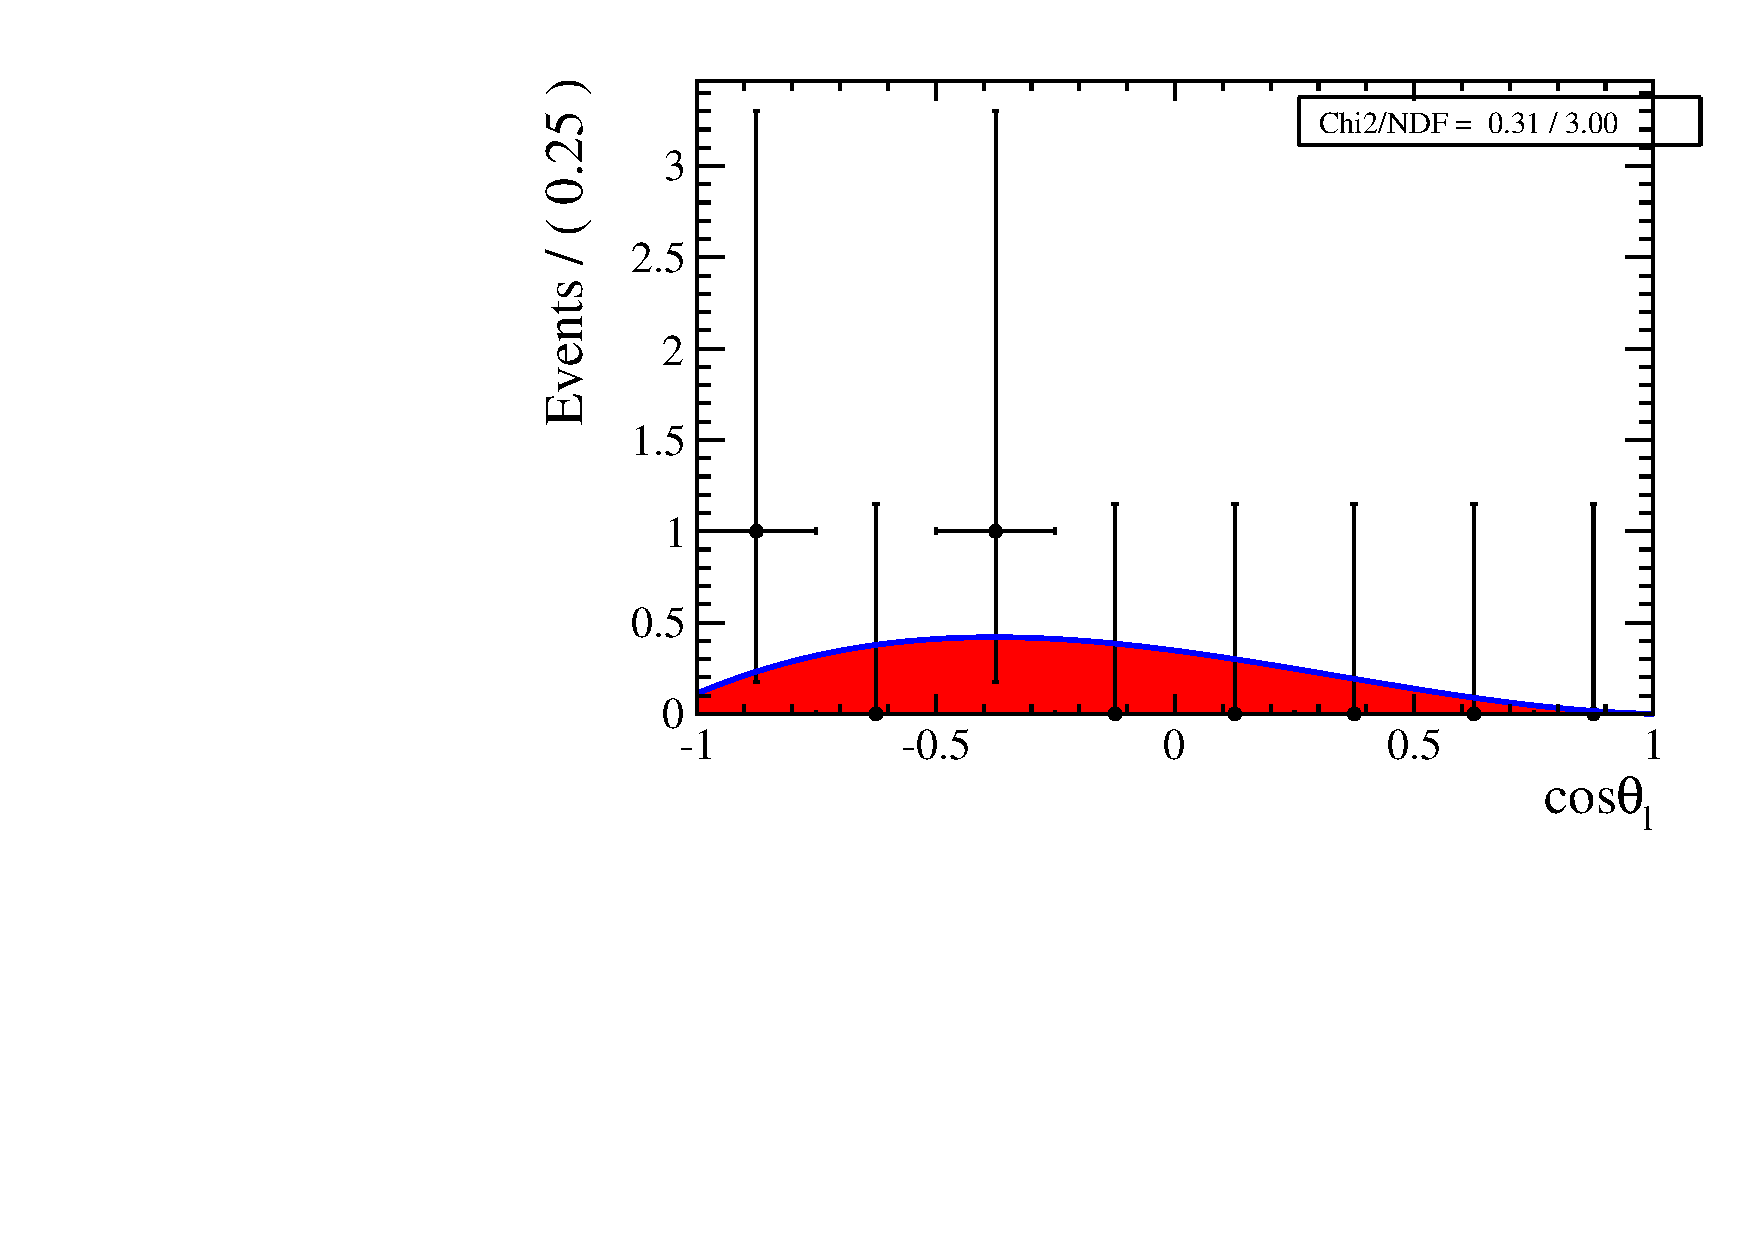
\includegraphics[width=0.40\textwidth]{Lmumu/figs/Side_LL_q2_010_200.pdf} \\
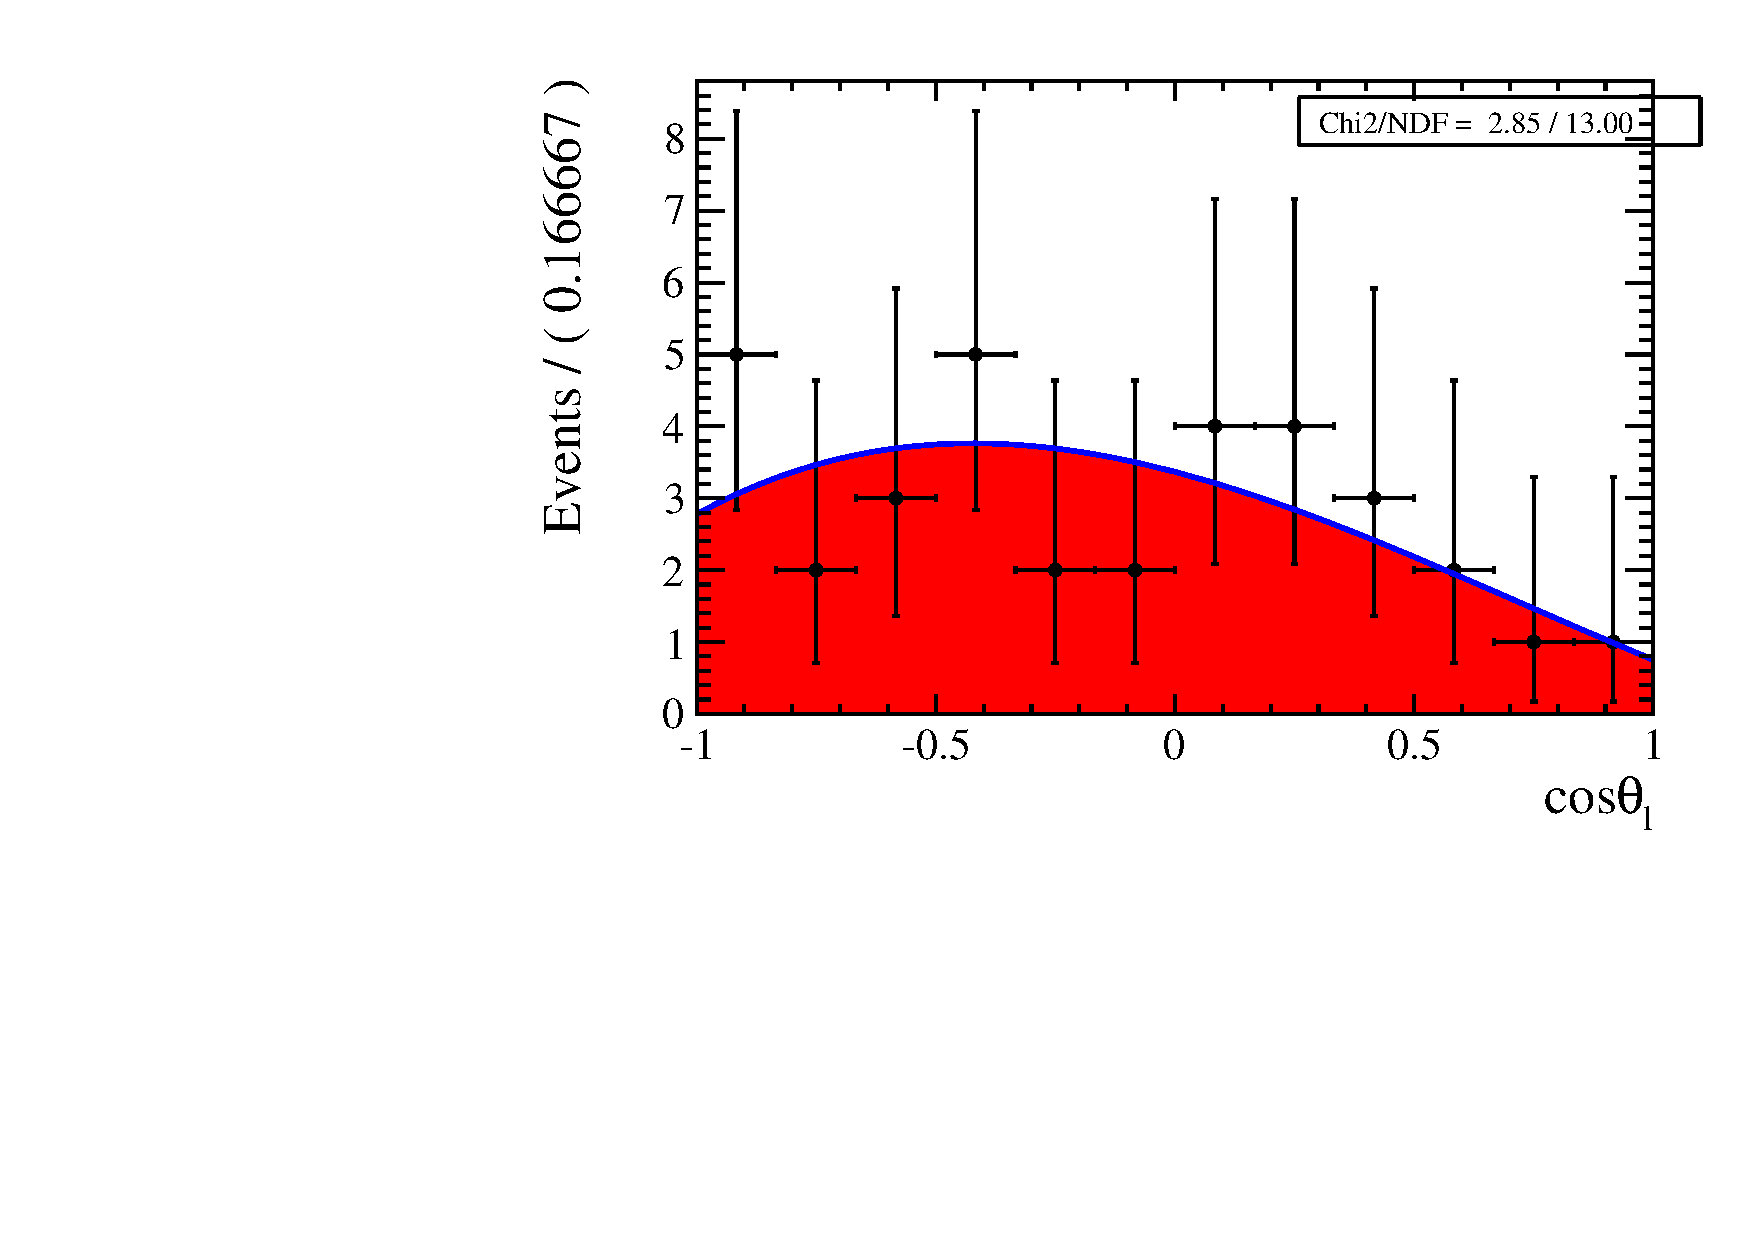
\includegraphics[width=0.40\textwidth]{Lmumu/figs/SideB_DD_q2_010_200.pdf}
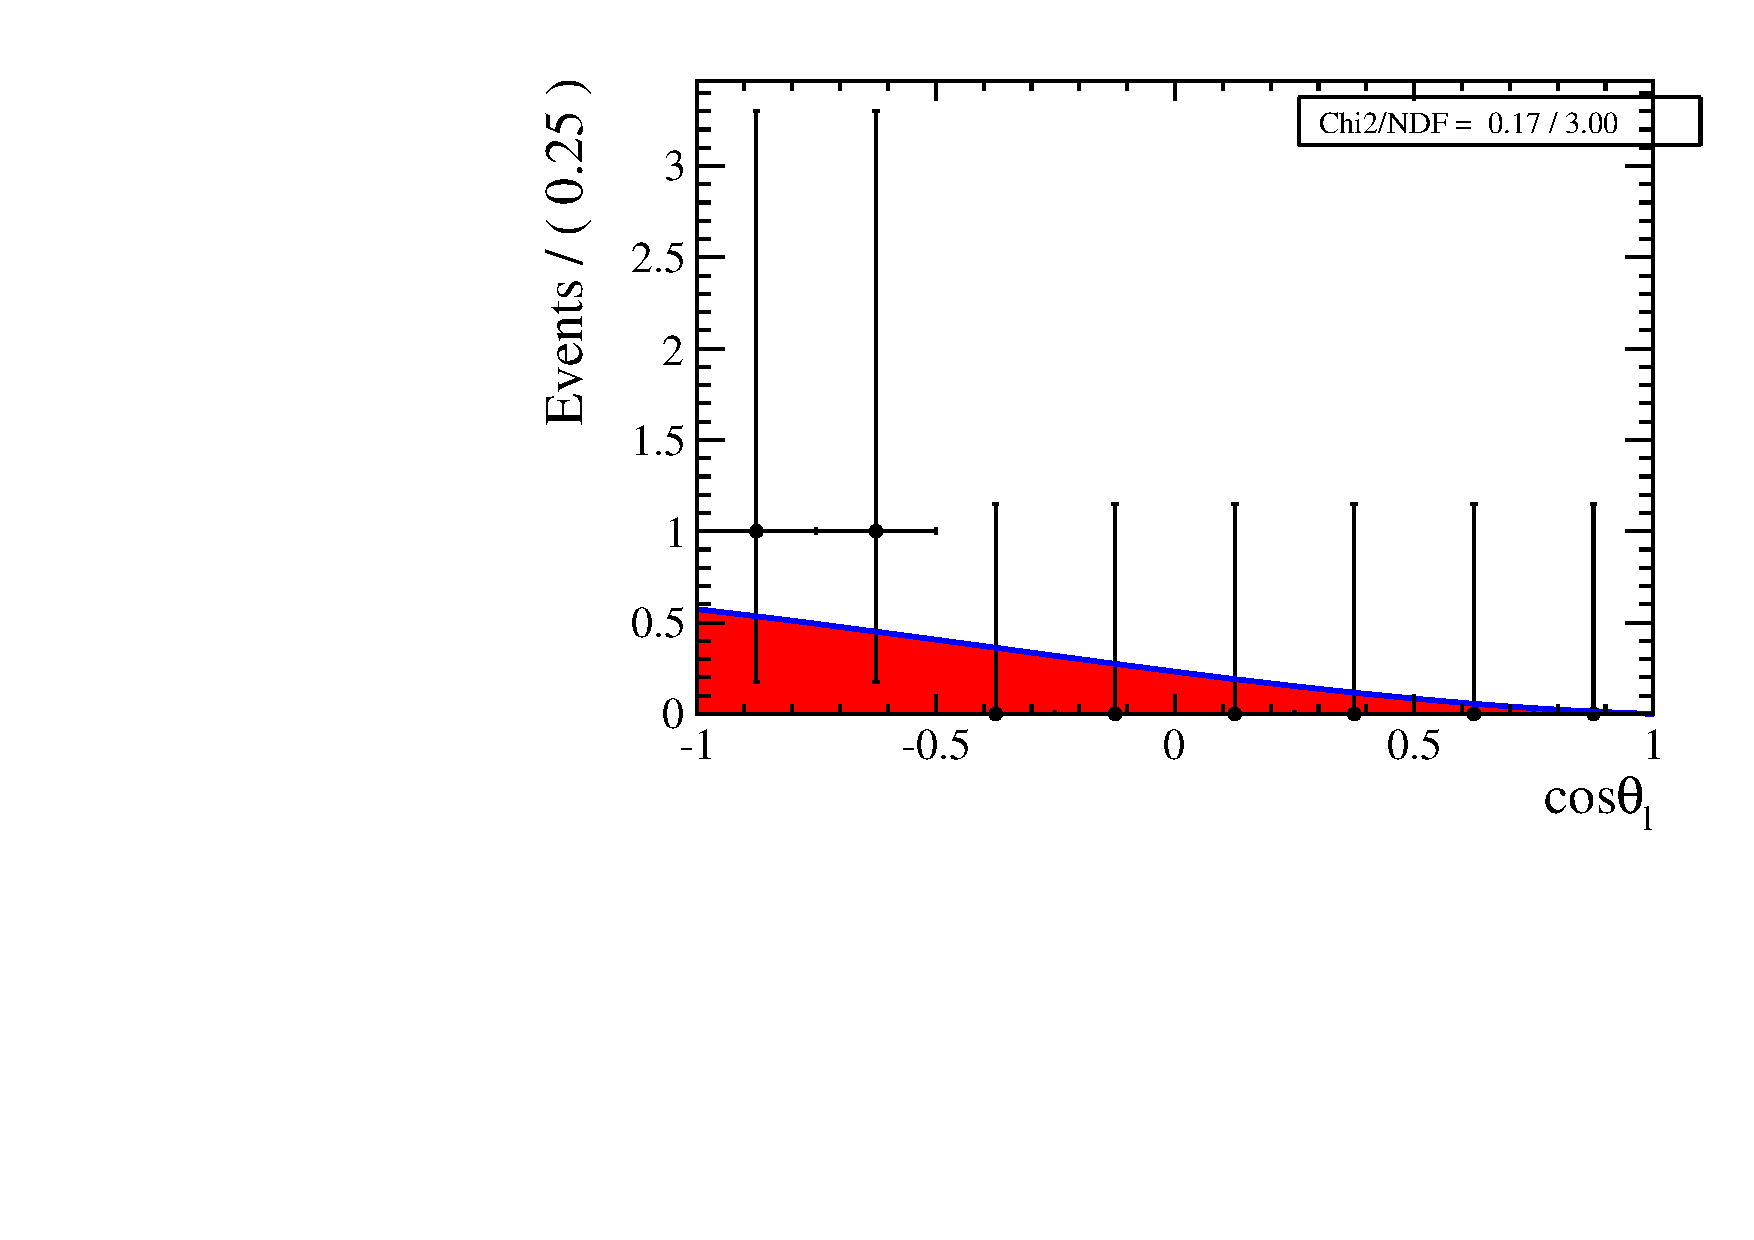
\includegraphics[width=0.40\textwidth]{Lmumu/figs/SideB_LL_q2_010_200.pdf}
\caption{Angular distribution in the sideband ($m_{\Lambda\mumu} > 5700 \mevcc$) as a function of $\cos\theta_\Lambda$ (top) and $\cos\theta_\Lambda$ (bottom) for down-down (left) and long-long (right) for events in the $0.1-2.0$GeV^2/c^2$$ \qsq bin.  }
\end{figure}


%%%%%%%%%%%%%%%%%%%%%%%%%%%%%%%%%%%%%%%%%%%%%%%%%%%%%%

\begin{figure}[!htb]
\centering
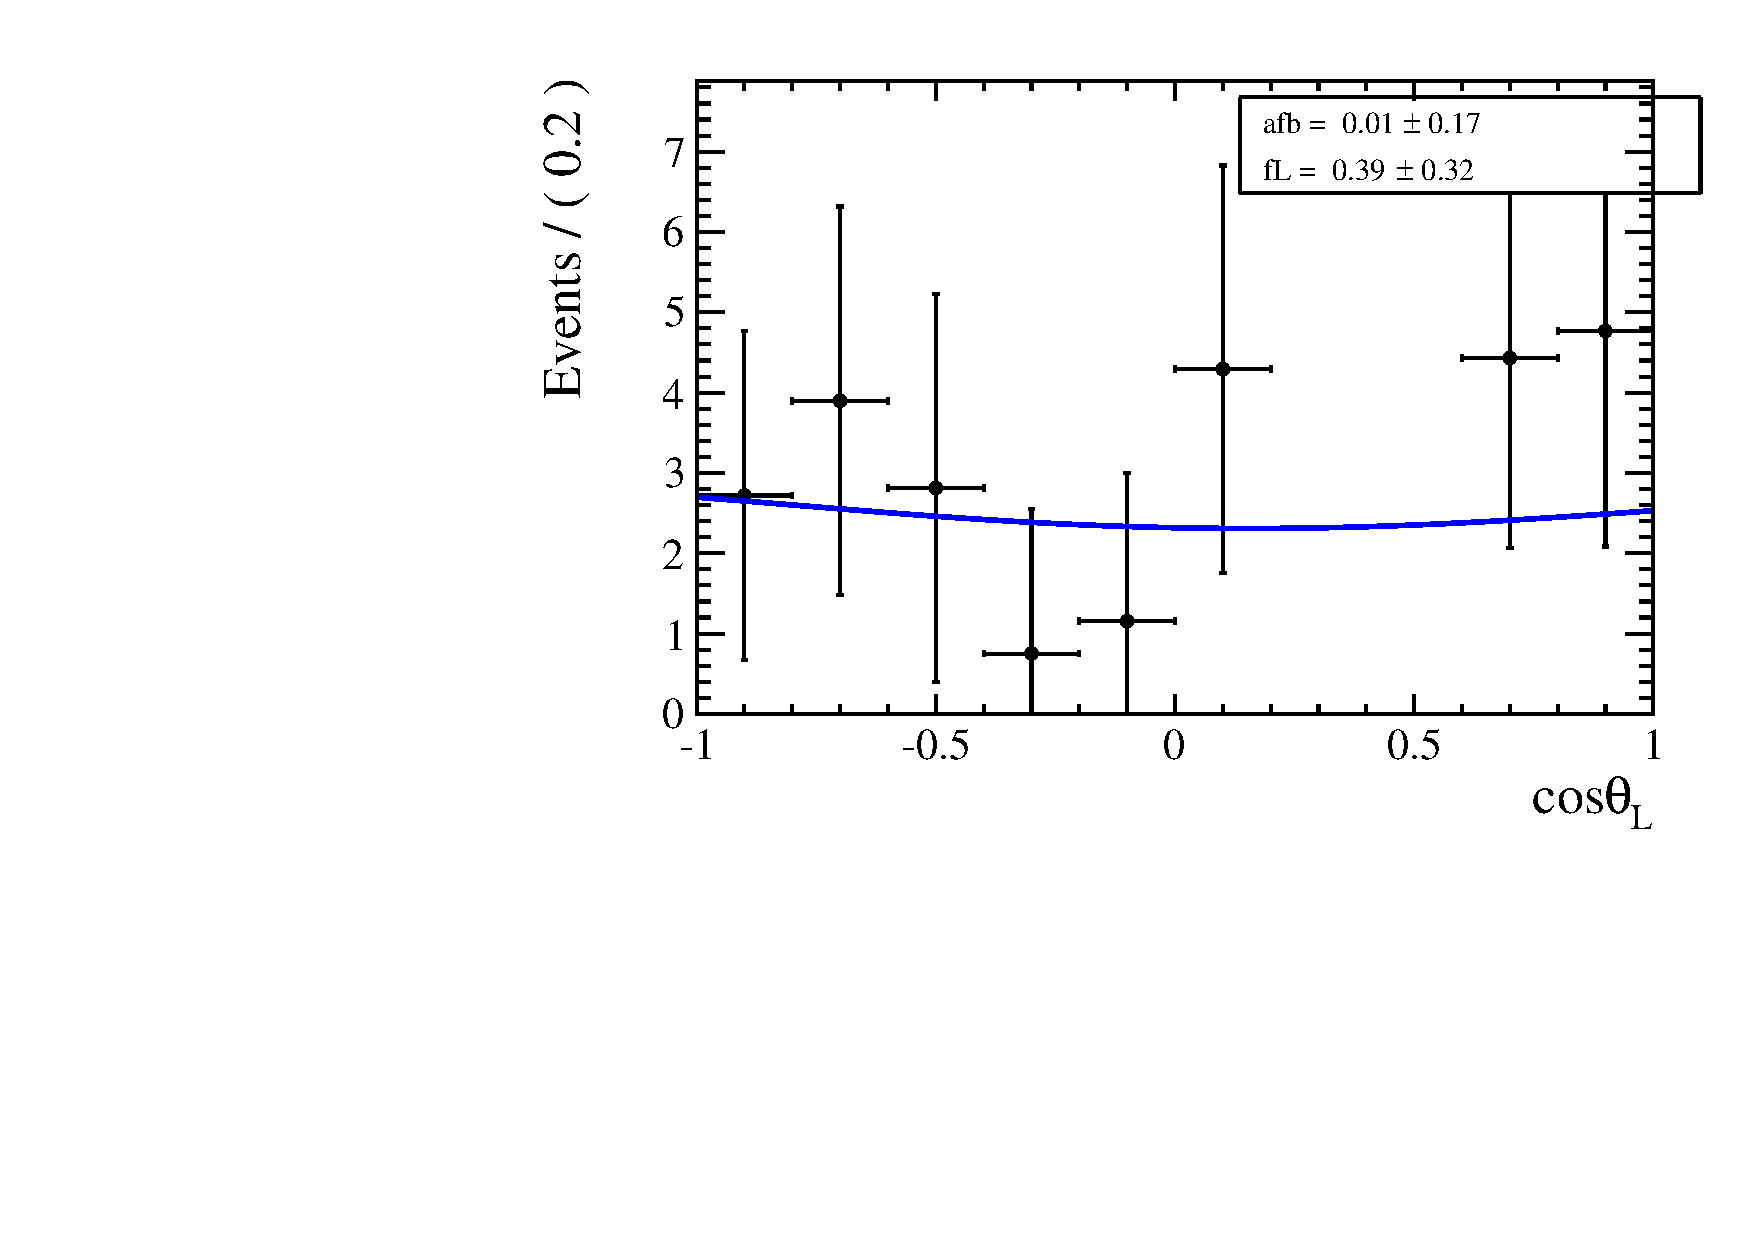
\includegraphics[width=0.40\textwidth]{Lmumu/figs/Afb_DD_q2_1100_1250.pdf}
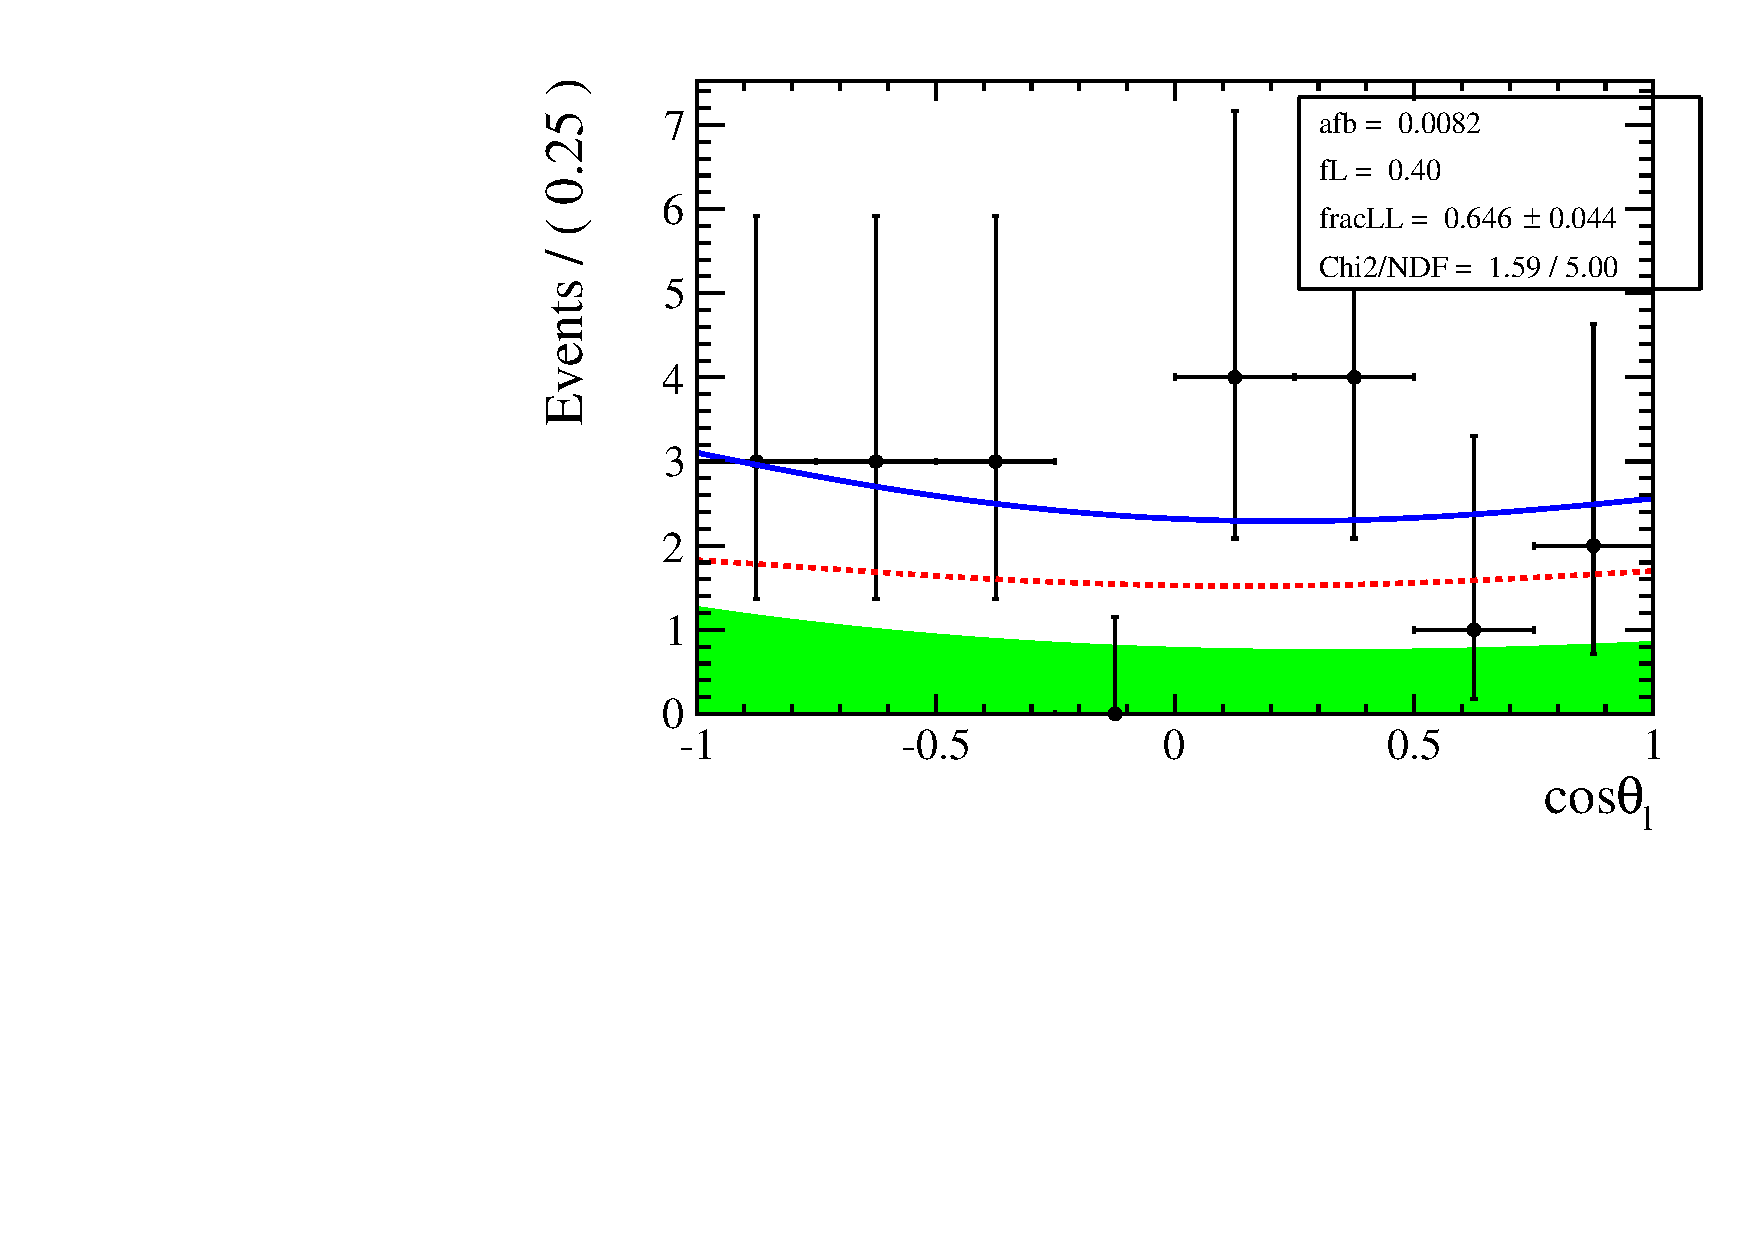
\includegraphics[width=0.40\textwidth]{Lmumu/figs/Afb_LL_q2_1100_1250.pdf} \\
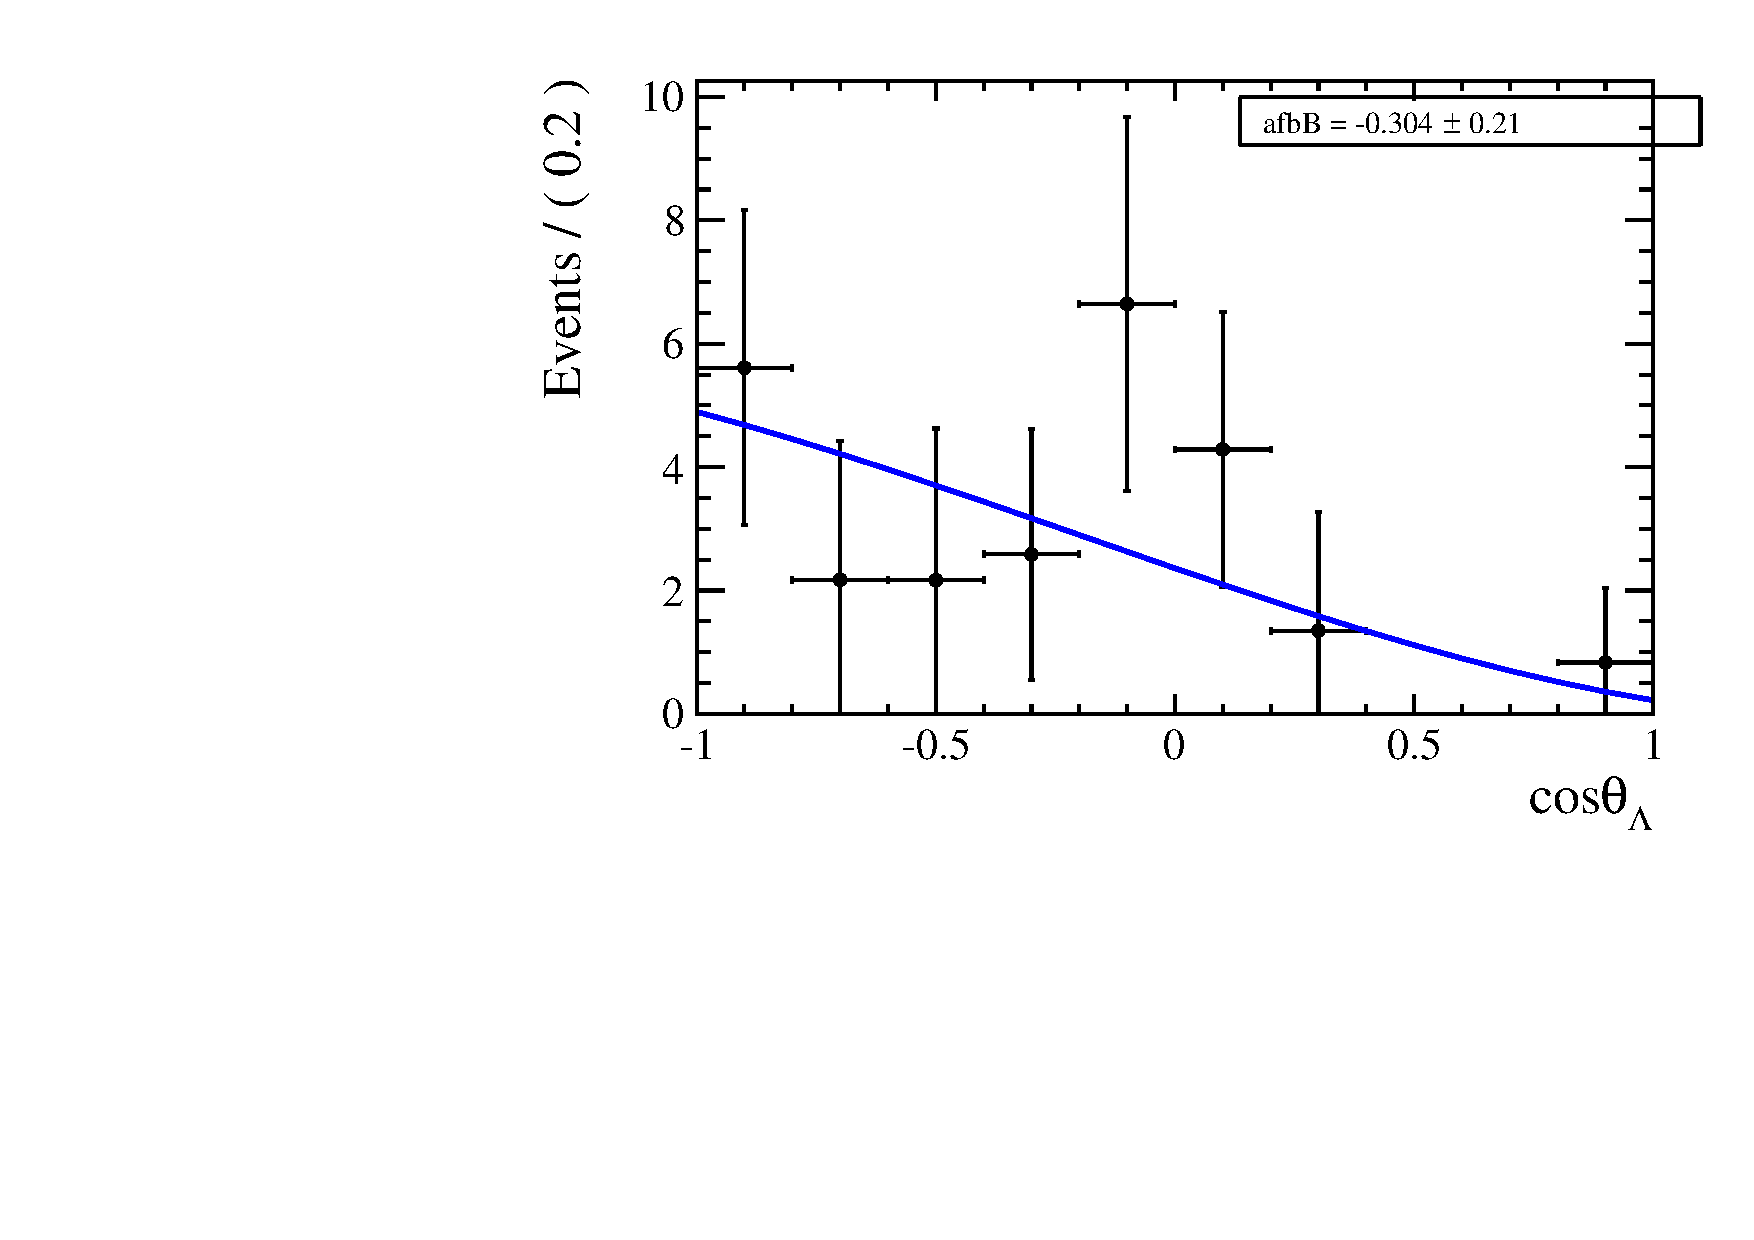
\includegraphics[width=0.40\textwidth]{Lmumu/figs/AfbB_DD_q2_1100_1250.pdf}
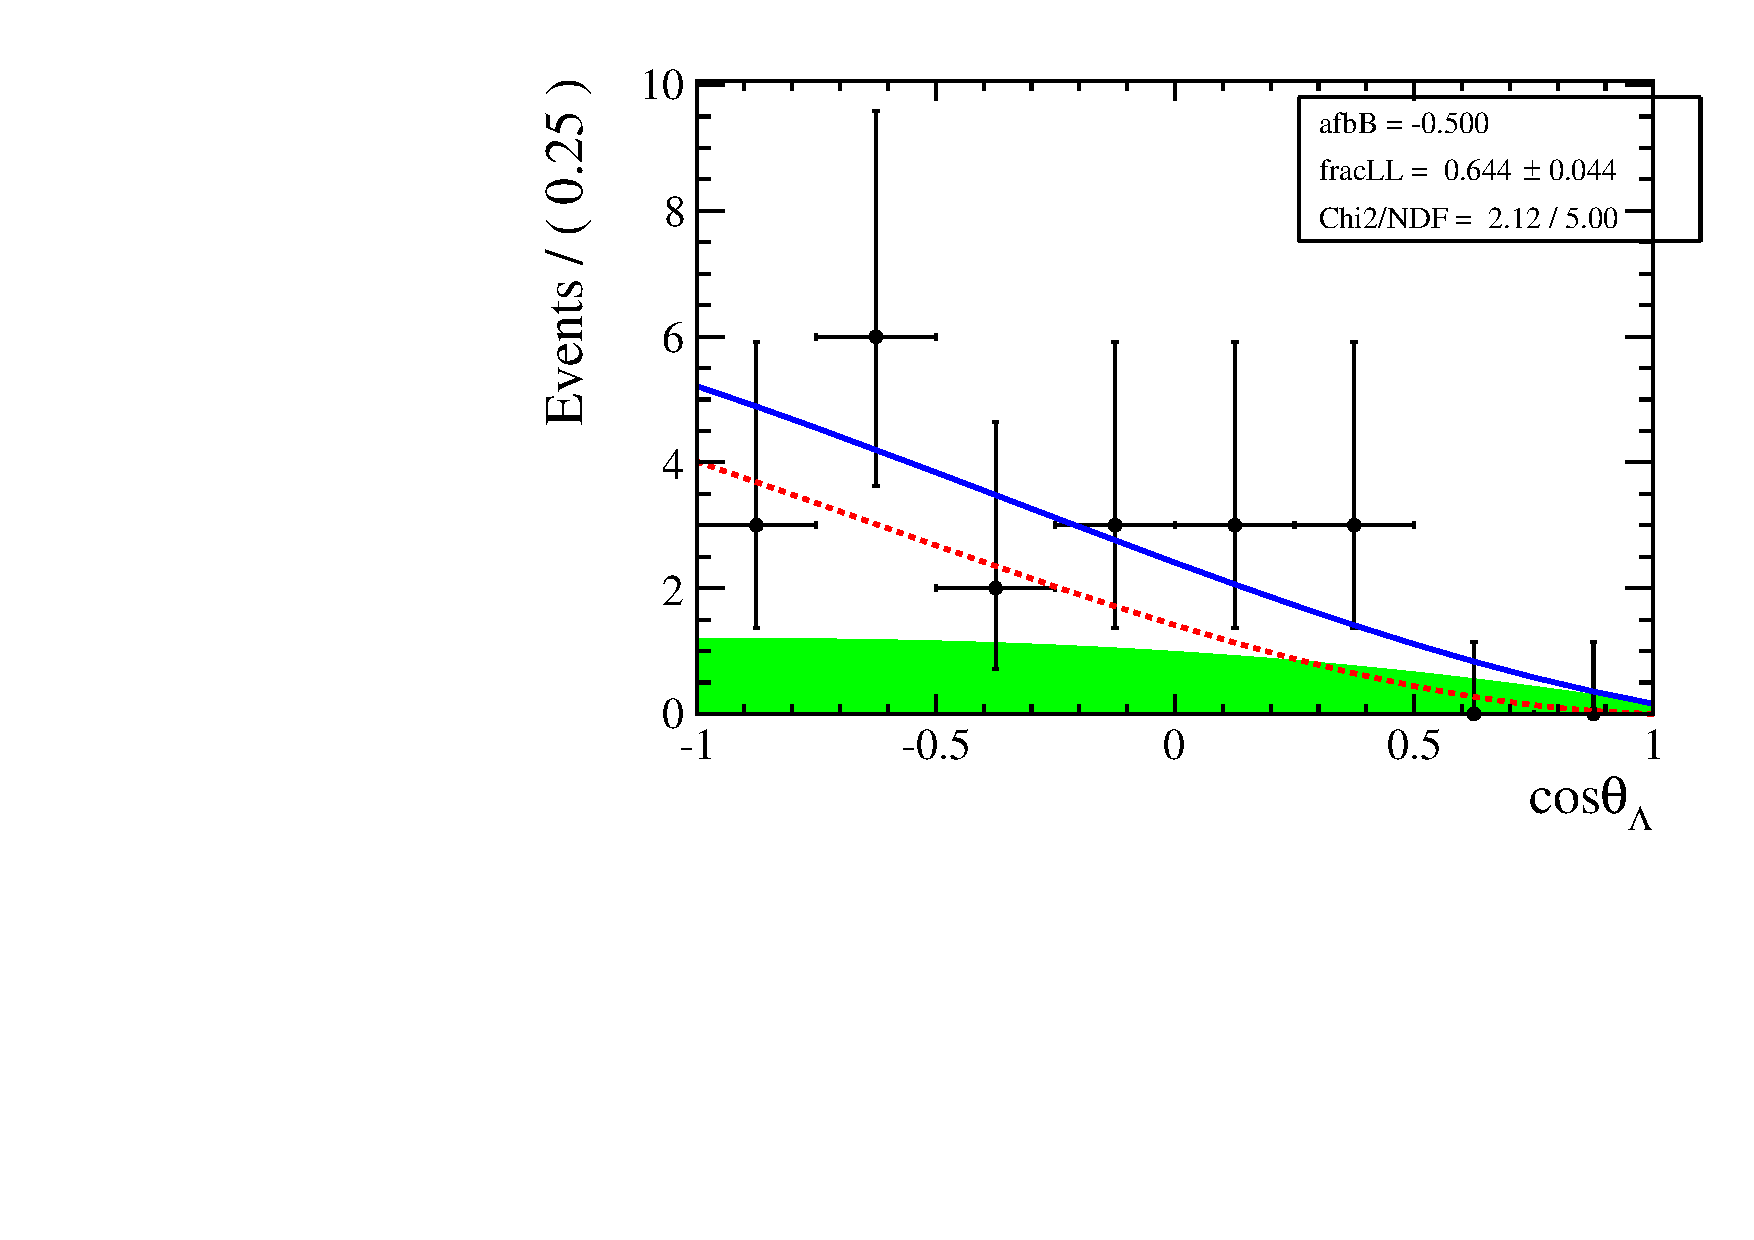
\includegraphics[width=0.40\textwidth]{Lmumu/figs/AfbB_LL_q2_1100_1250.pdf}
\caption{Fitted angular distribution as a function of $\cos\theta_\ell$ (top) and $\cos\theta_\Lambda$ (bottom) for down-down (left) and long-long (right) events for events in the $11.0-12.5$GeV^2/c^2$$ \qsq bin.  }
\end{figure}




\begin{figure}[!htb]
\centering
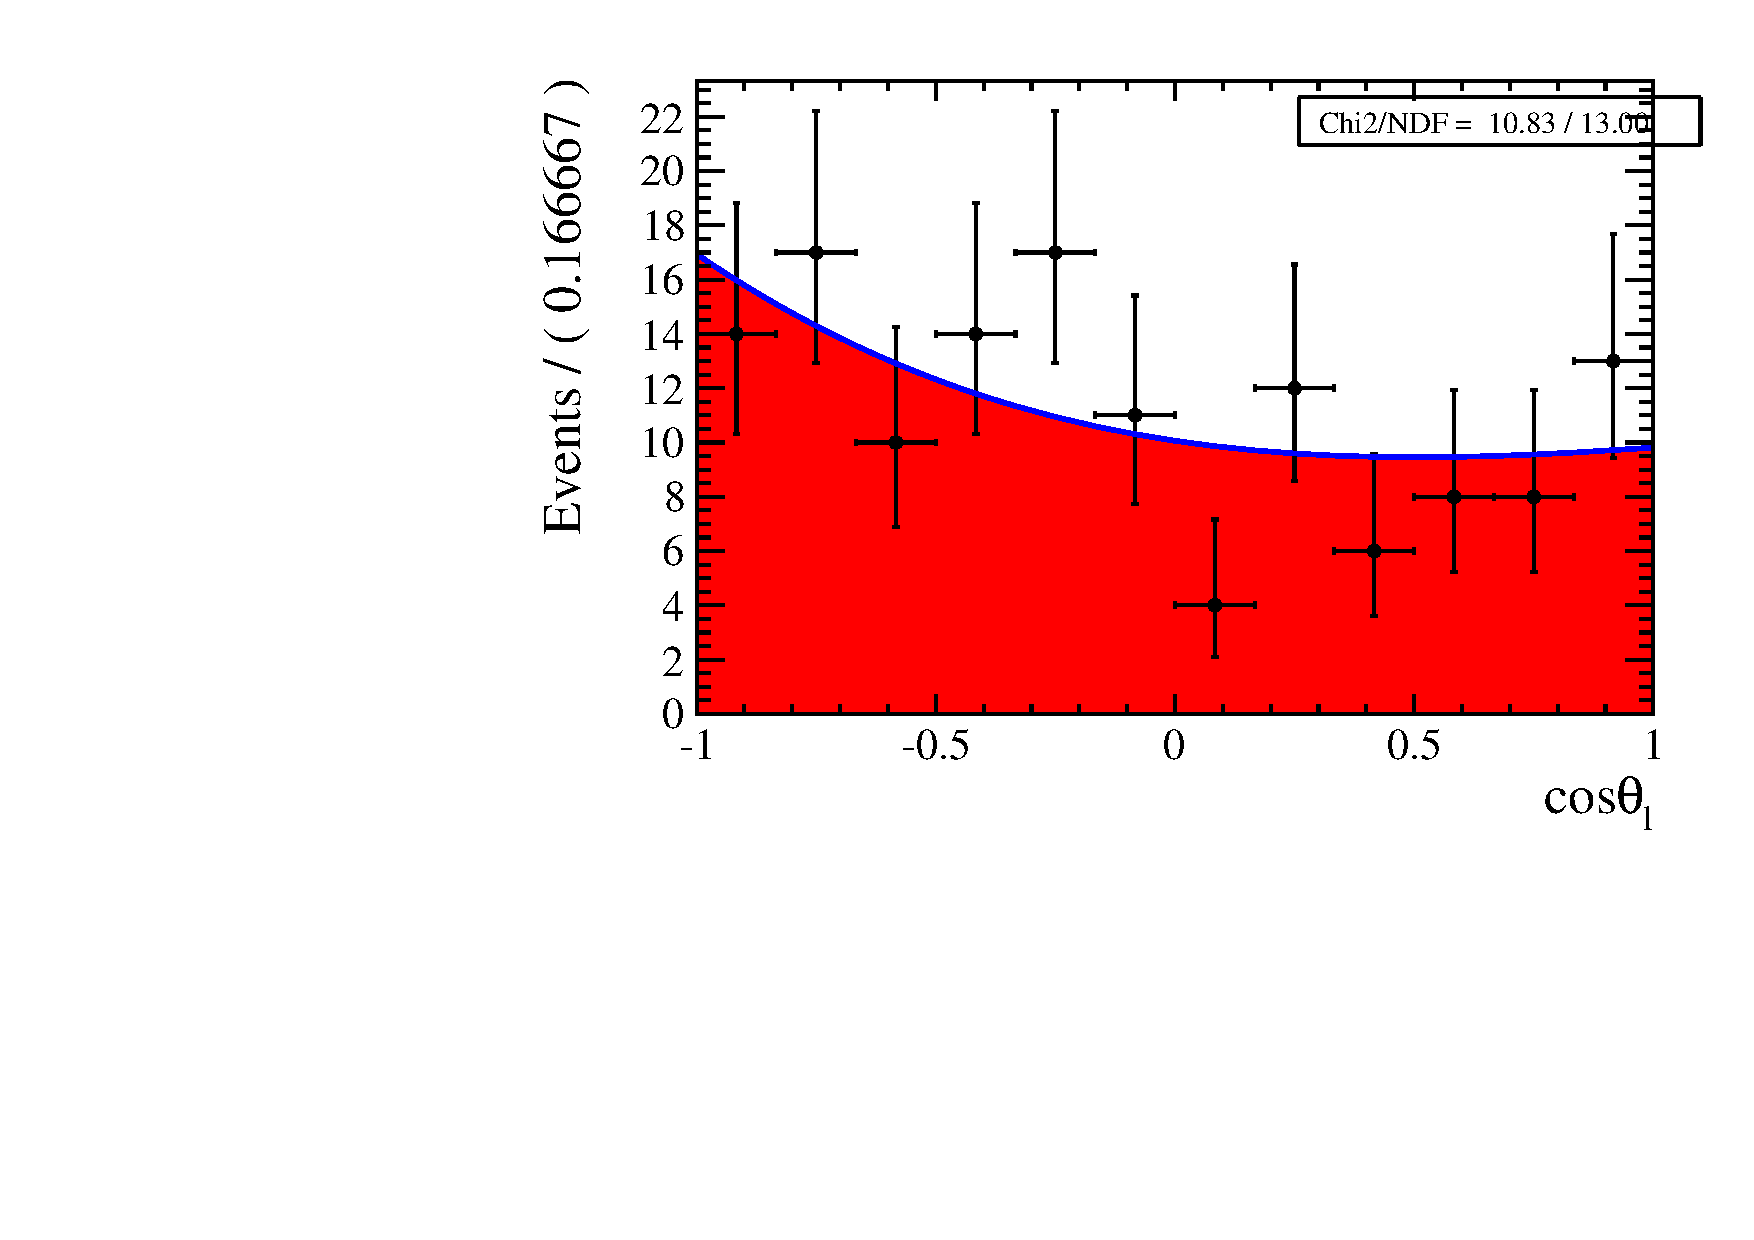
\includegraphics[width=0.40\textwidth]{Lmumu/figs/Side_DD_q2_1100_1250.pdf}
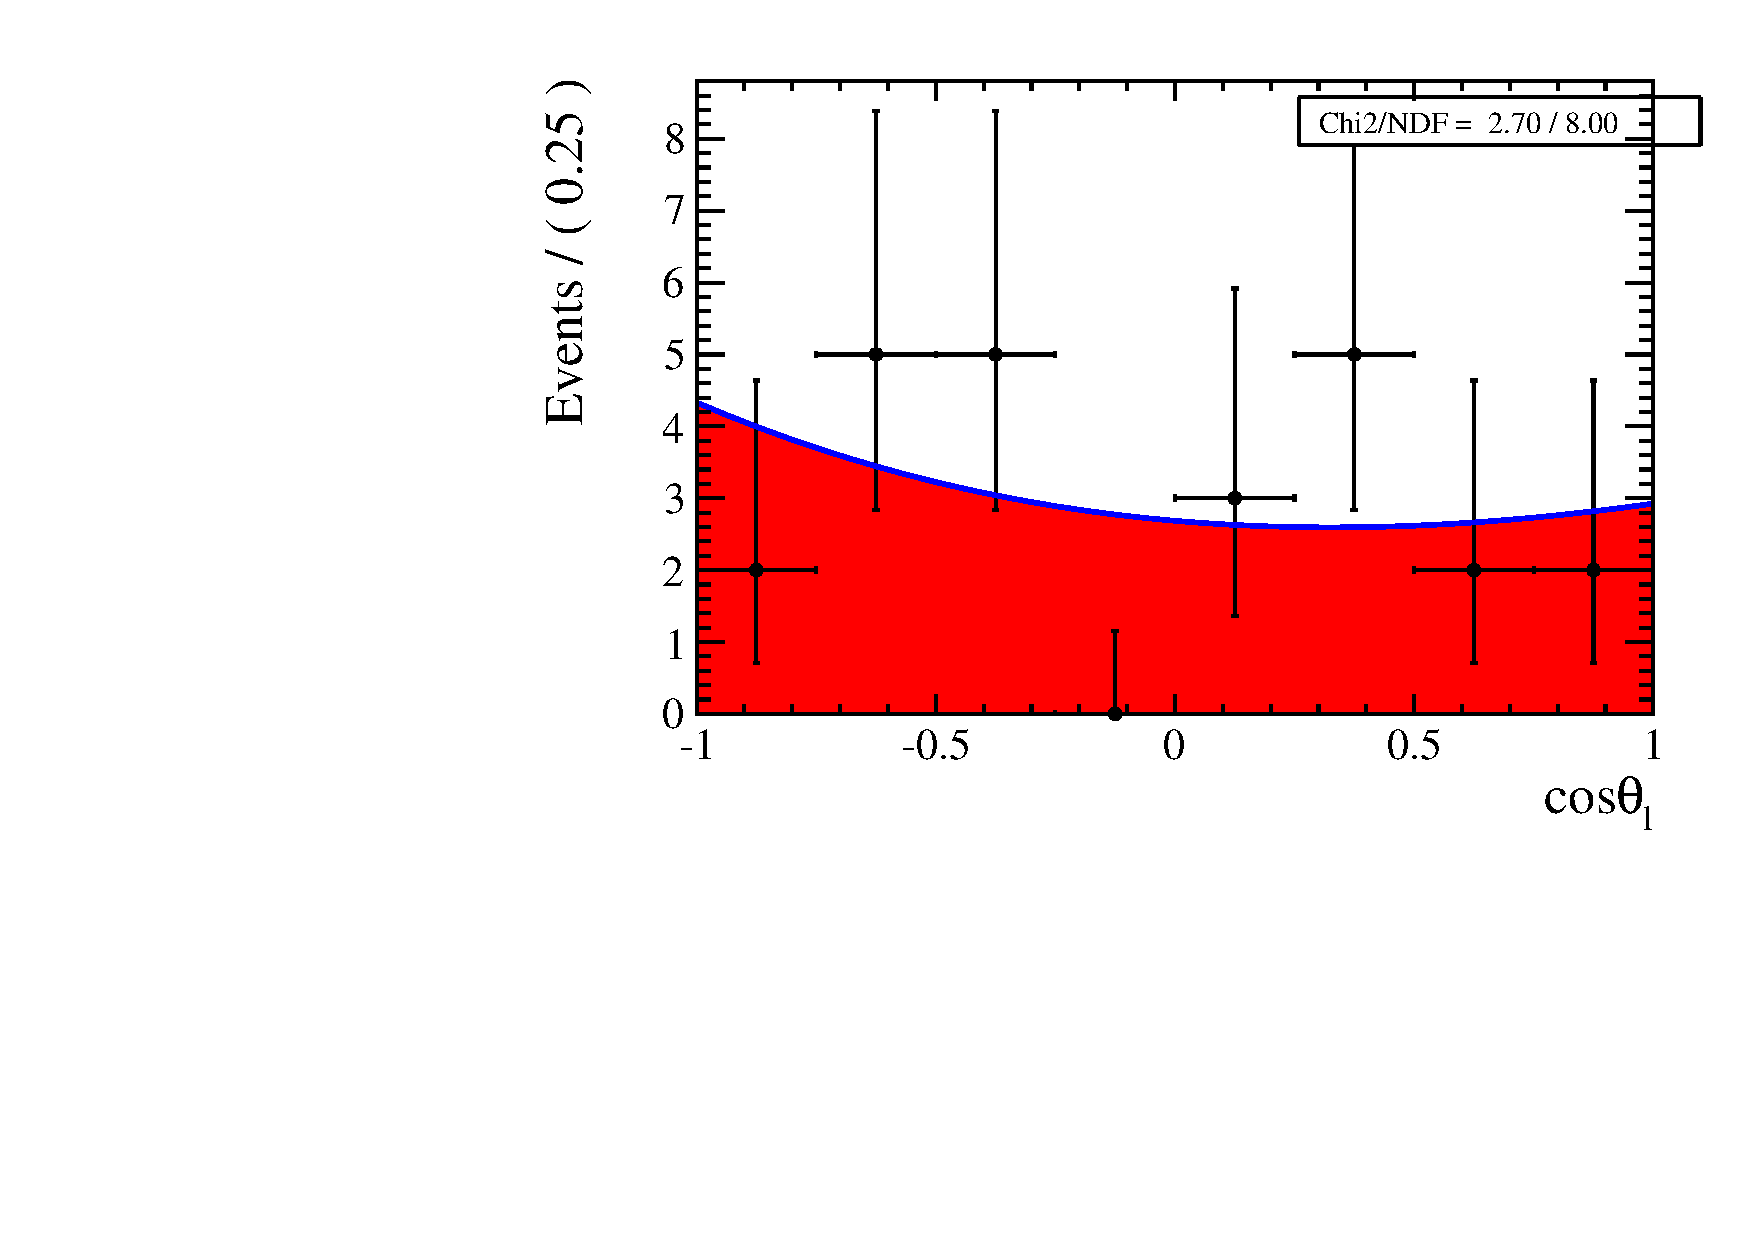
\includegraphics[width=0.40\textwidth]{Lmumu/figs/Side_LL_q2_1100_1250.pdf} \\
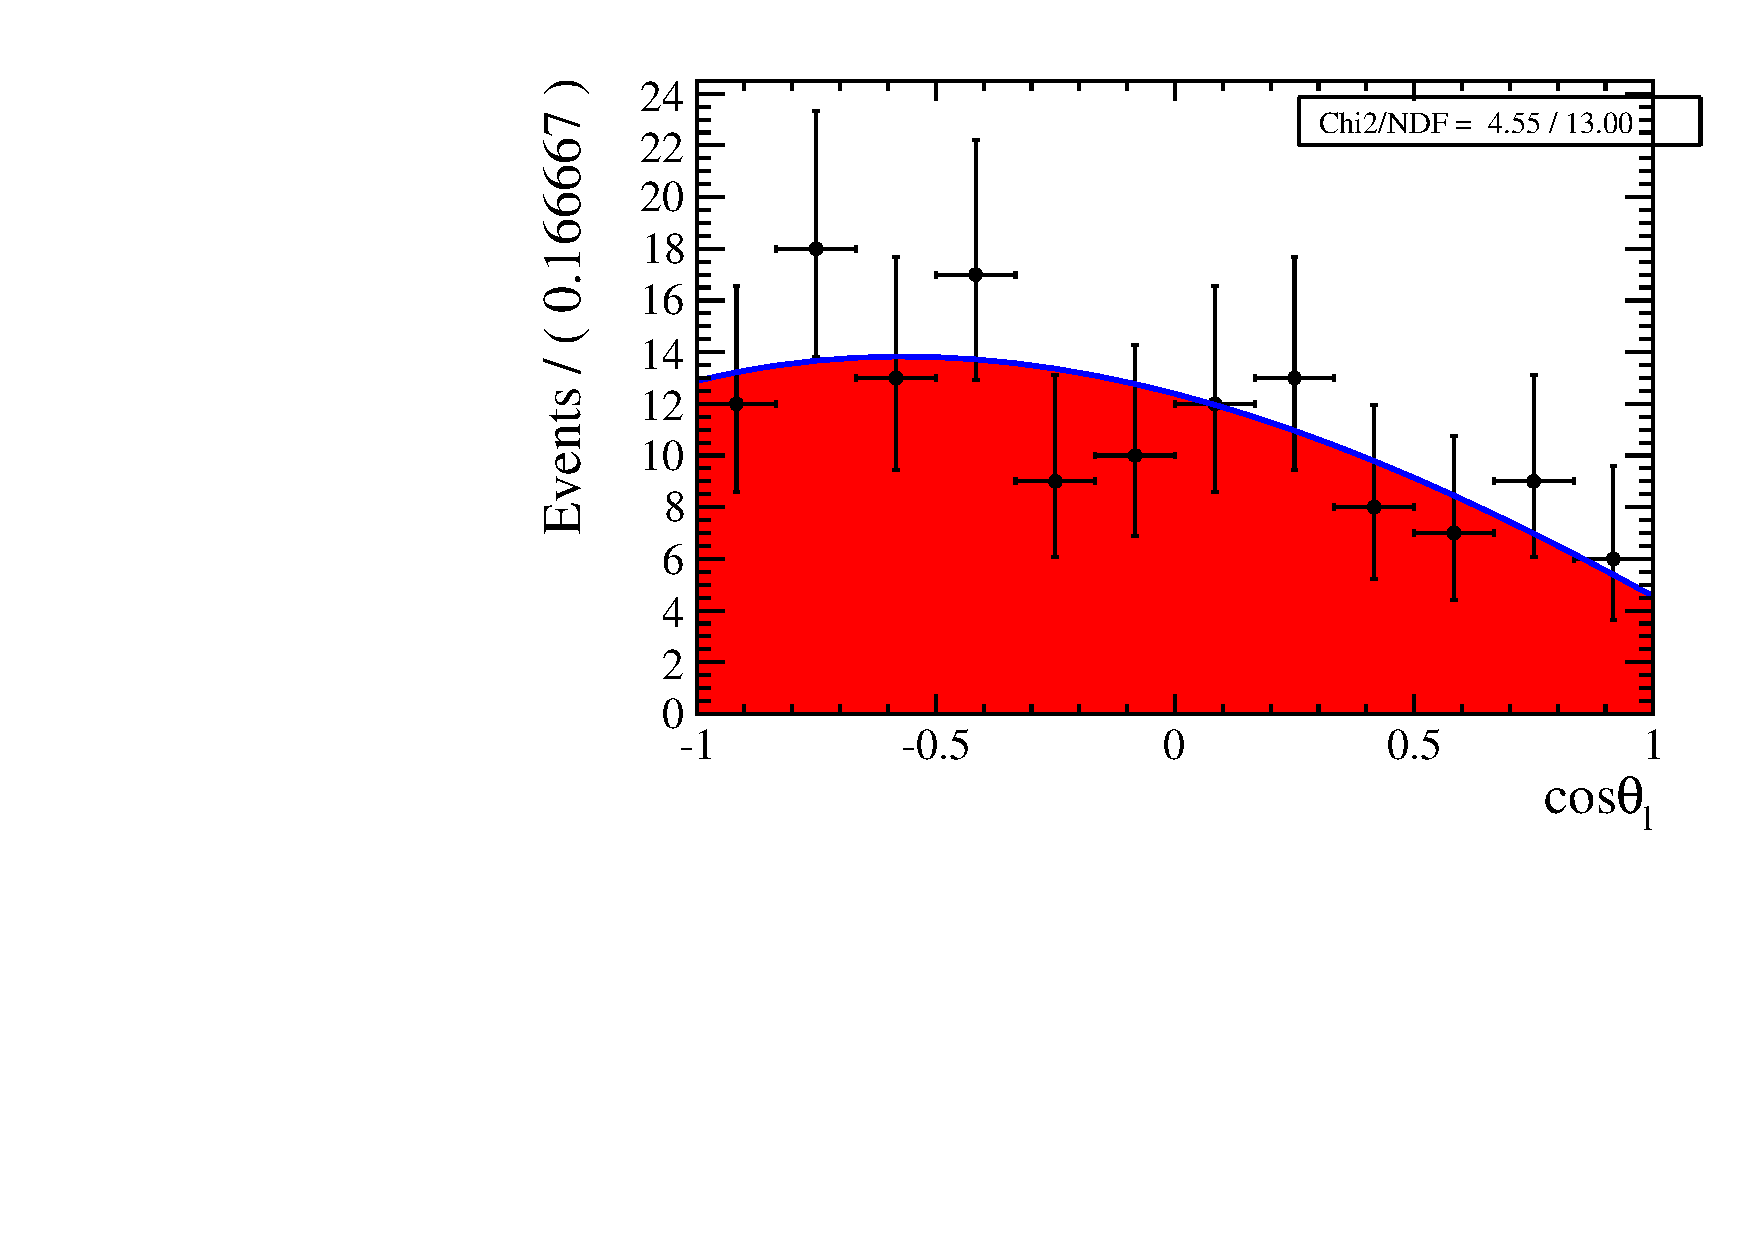
\includegraphics[width=0.40\textwidth]{Lmumu/figs/SideB_DD_q2_1100_1250.pdf}
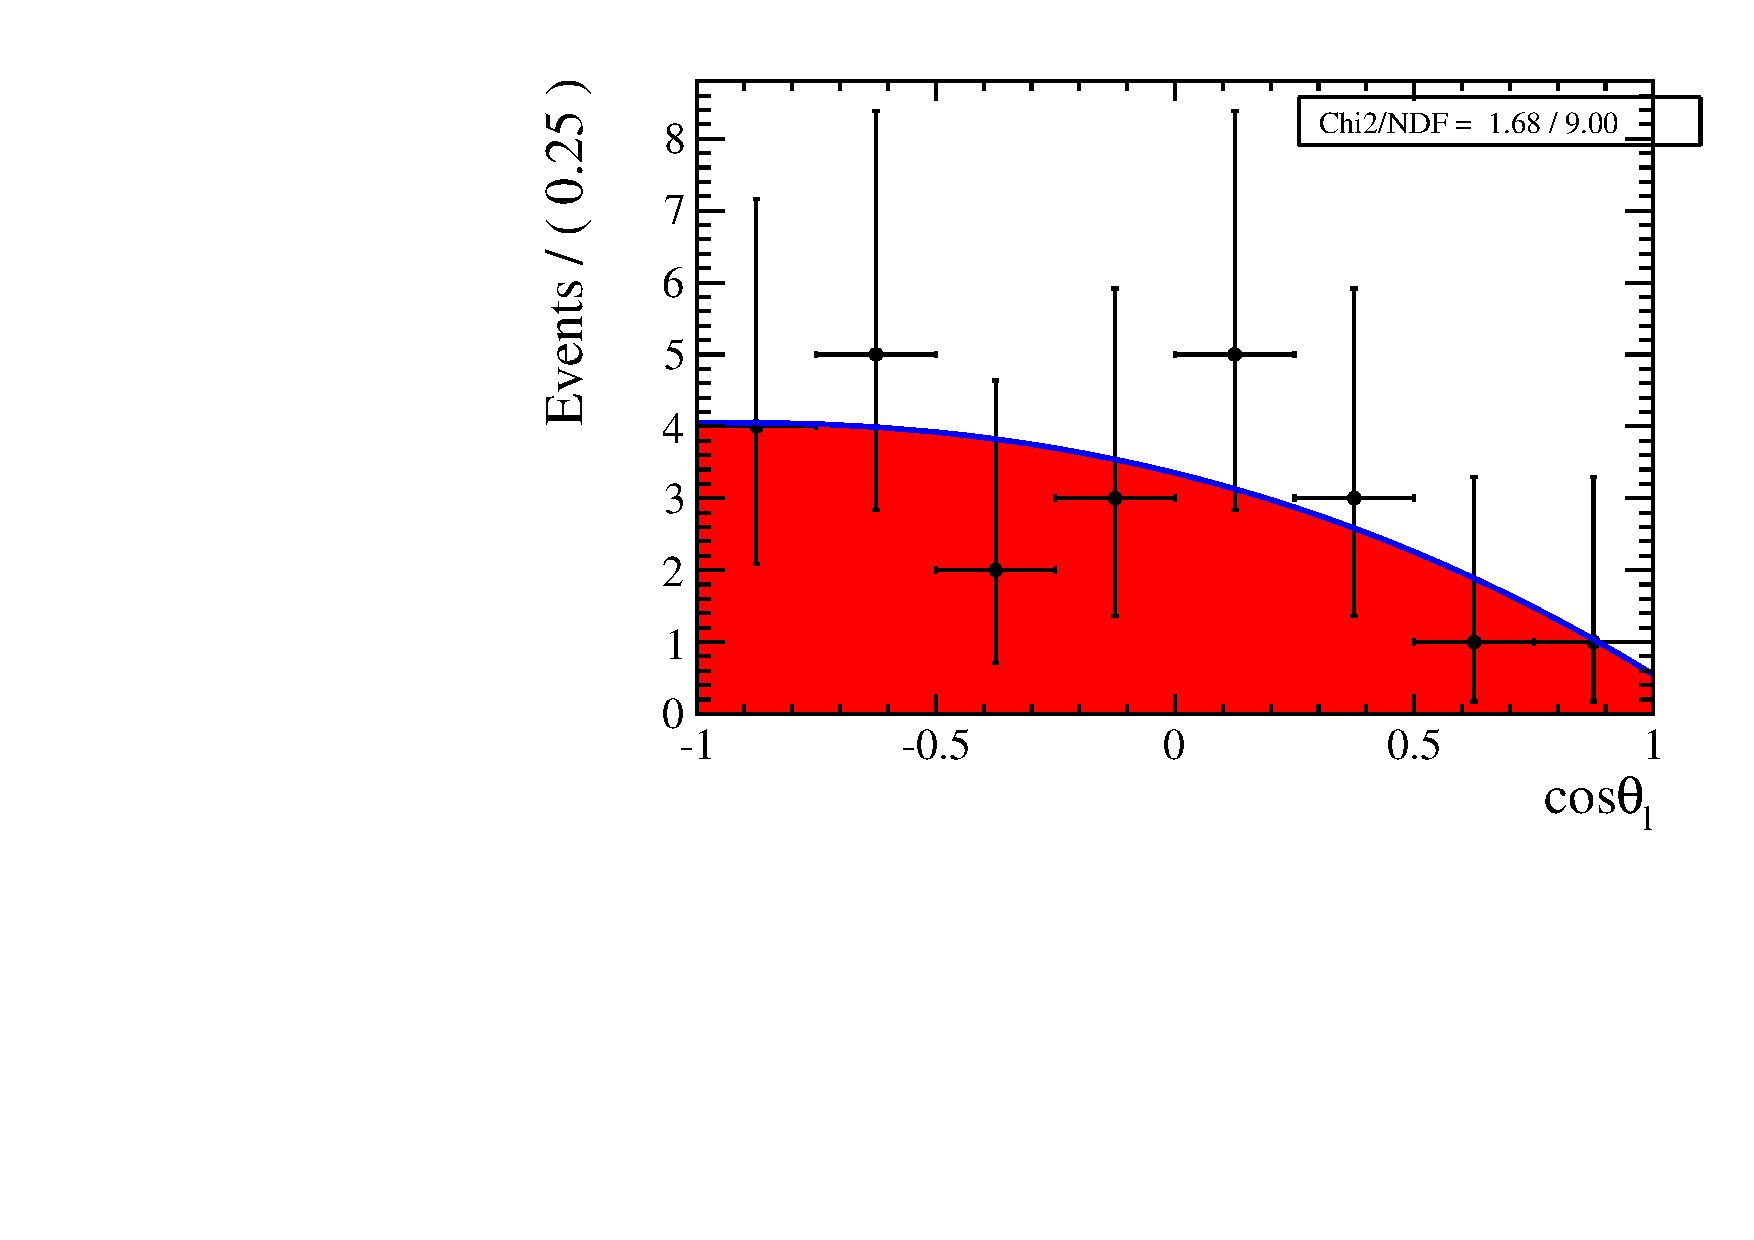
\includegraphics[width=0.40\textwidth]{Lmumu/figs/SideB_LL_q2_1100_1250.pdf}
\caption{Angular distribution in the sideband ($m_{\Lambda\mumu} > 5700 \mevcc$) as a function of $\cos\theta_\Lambda$ (top) and $\cos\theta_\Lambda$ (bottom) for down-down (left) and long-long (right) for events in the $11.0-12.5$GeV^2/c^2$$ \qsq bin.  }
\end{figure}


%%%%%%%%%%%%%%%%%%%%%%%%%%%%%%%%%%%%%%%%%%%%%%%%%%%%%%%%


\begin{figure}[!htb]
\centering
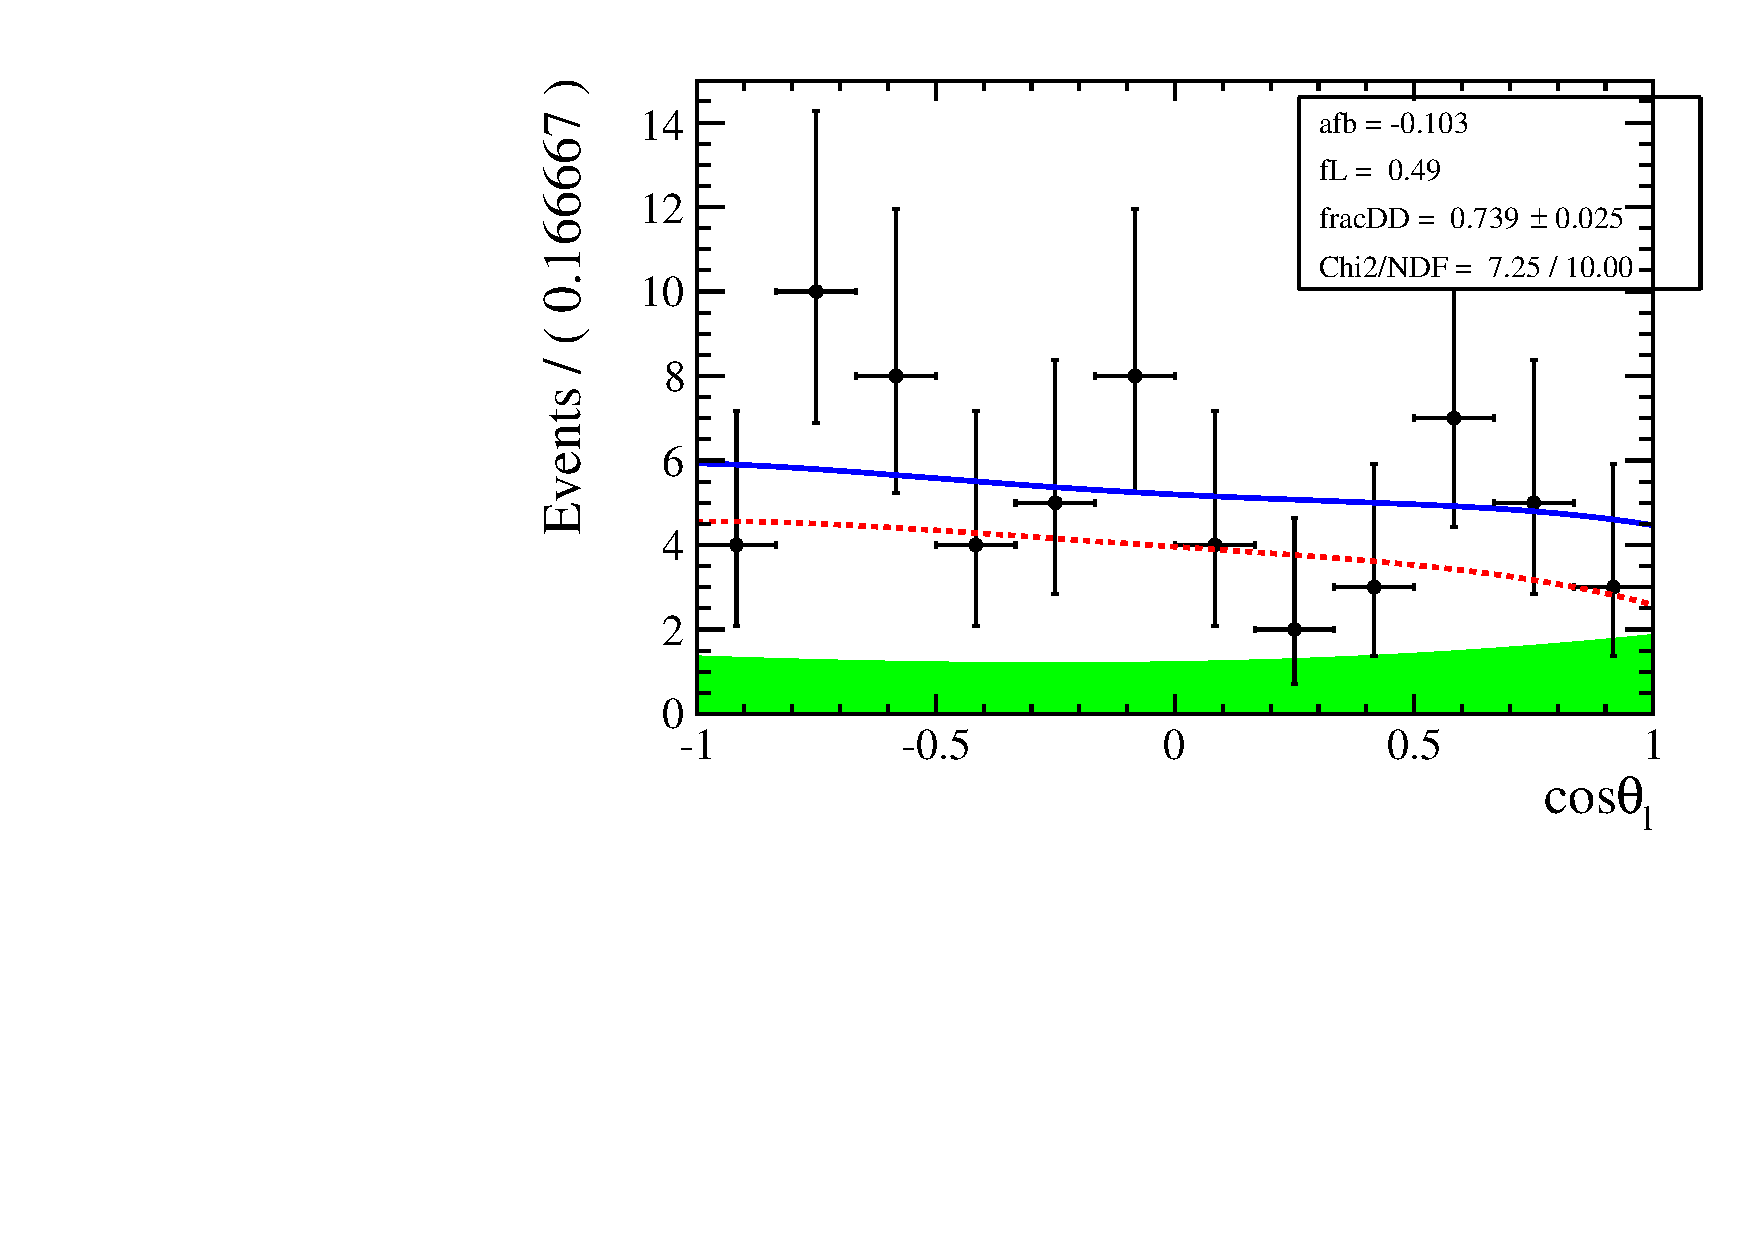
\includegraphics[width=0.40\textwidth]{Lmumu/figs/Afb_DD_q2_1500_1600.pdf}
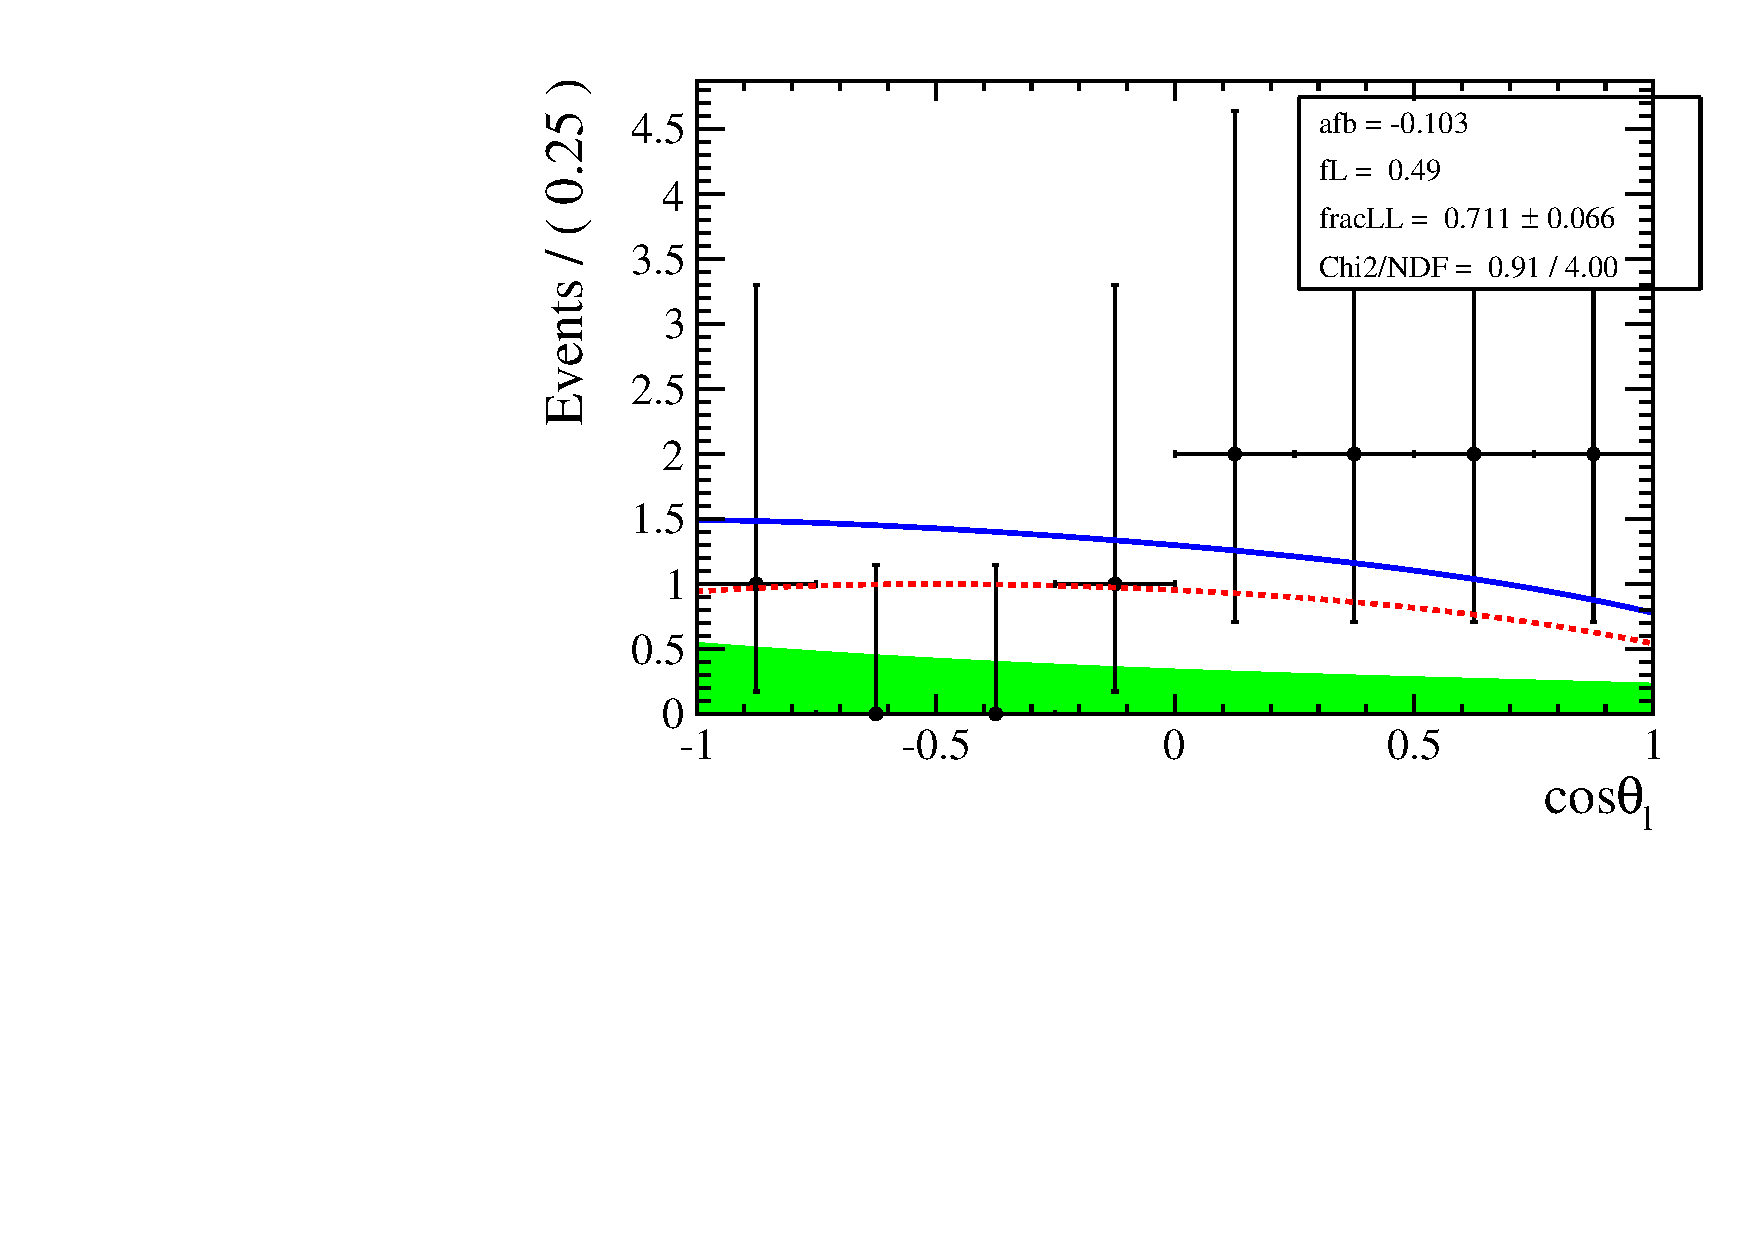
\includegraphics[width=0.40\textwidth]{Lmumu/figs/Afb_LL_q2_1500_1600.pdf} \\
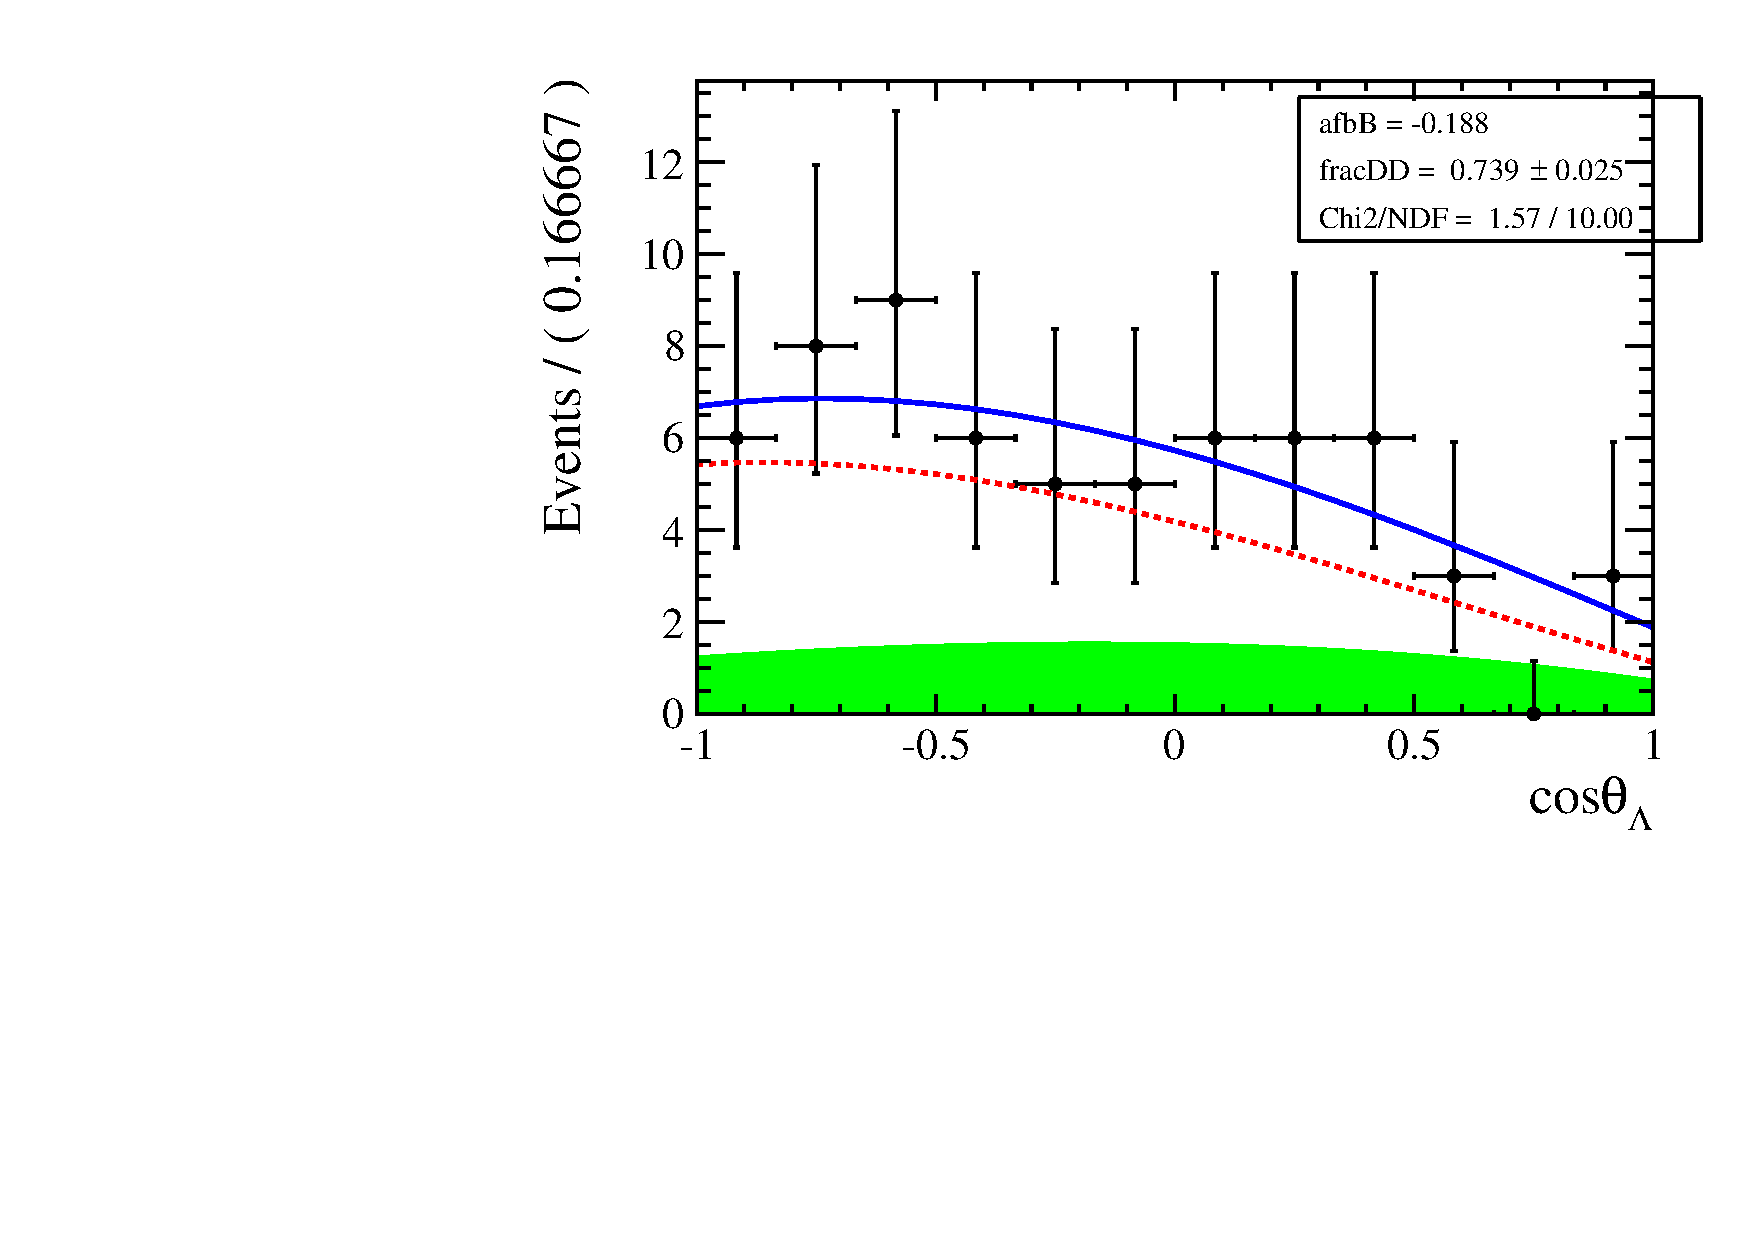
\includegraphics[width=0.40\textwidth]{Lmumu/figs/AfbB_DD_q2_1500_1600.pdf}
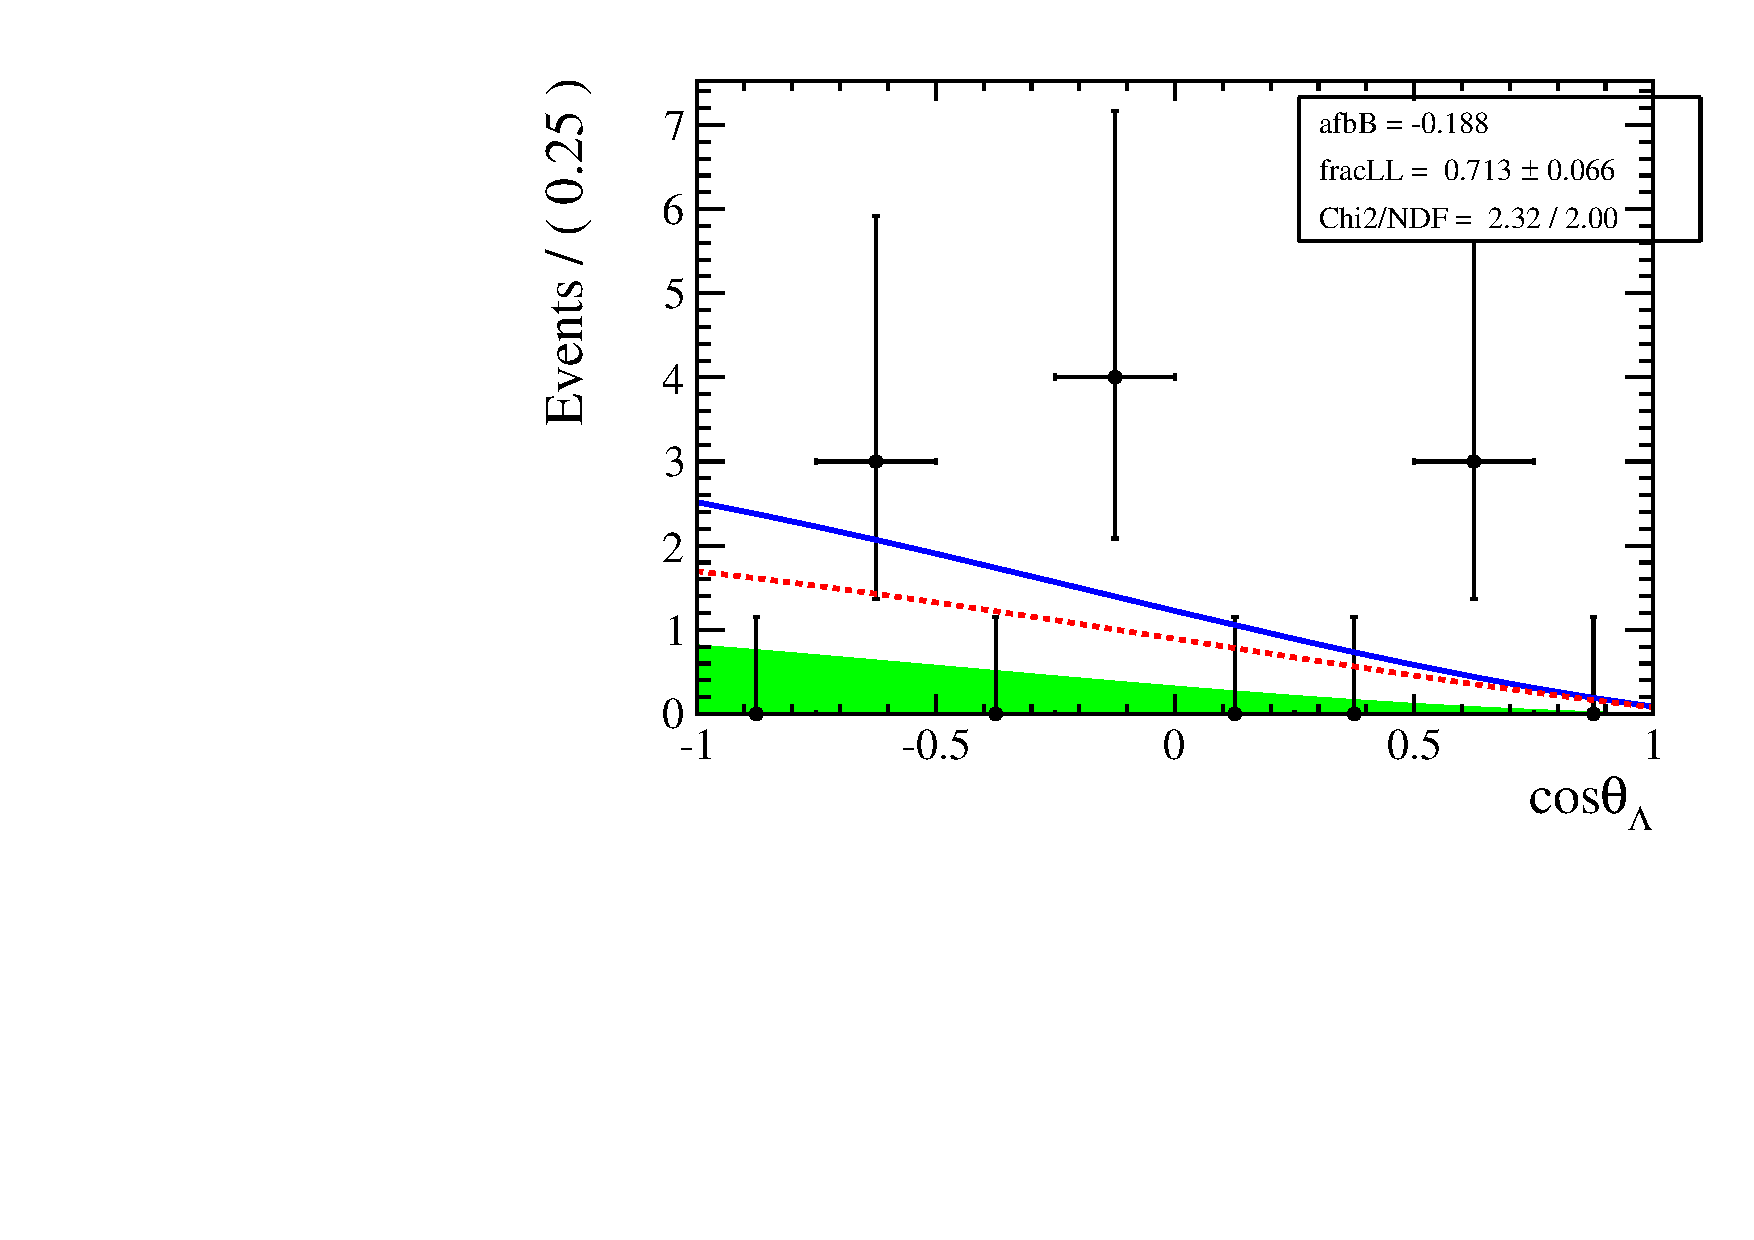
\includegraphics[width=0.40\textwidth]{Lmumu/figs/AfbB_LL_q2_1500_1600.pdf}
\caption{Fitted angular distribution as a function of $\cos\theta_\ell$ (top) and $\cos\theta_\Lambda$ (bottom) for down-down (left) and long-long (right) for events in the $15.0-16.0$GeV^2/c^2$$ \qsq bin.  }
\end{figure}



\begin{figure}[!htb]
\centering
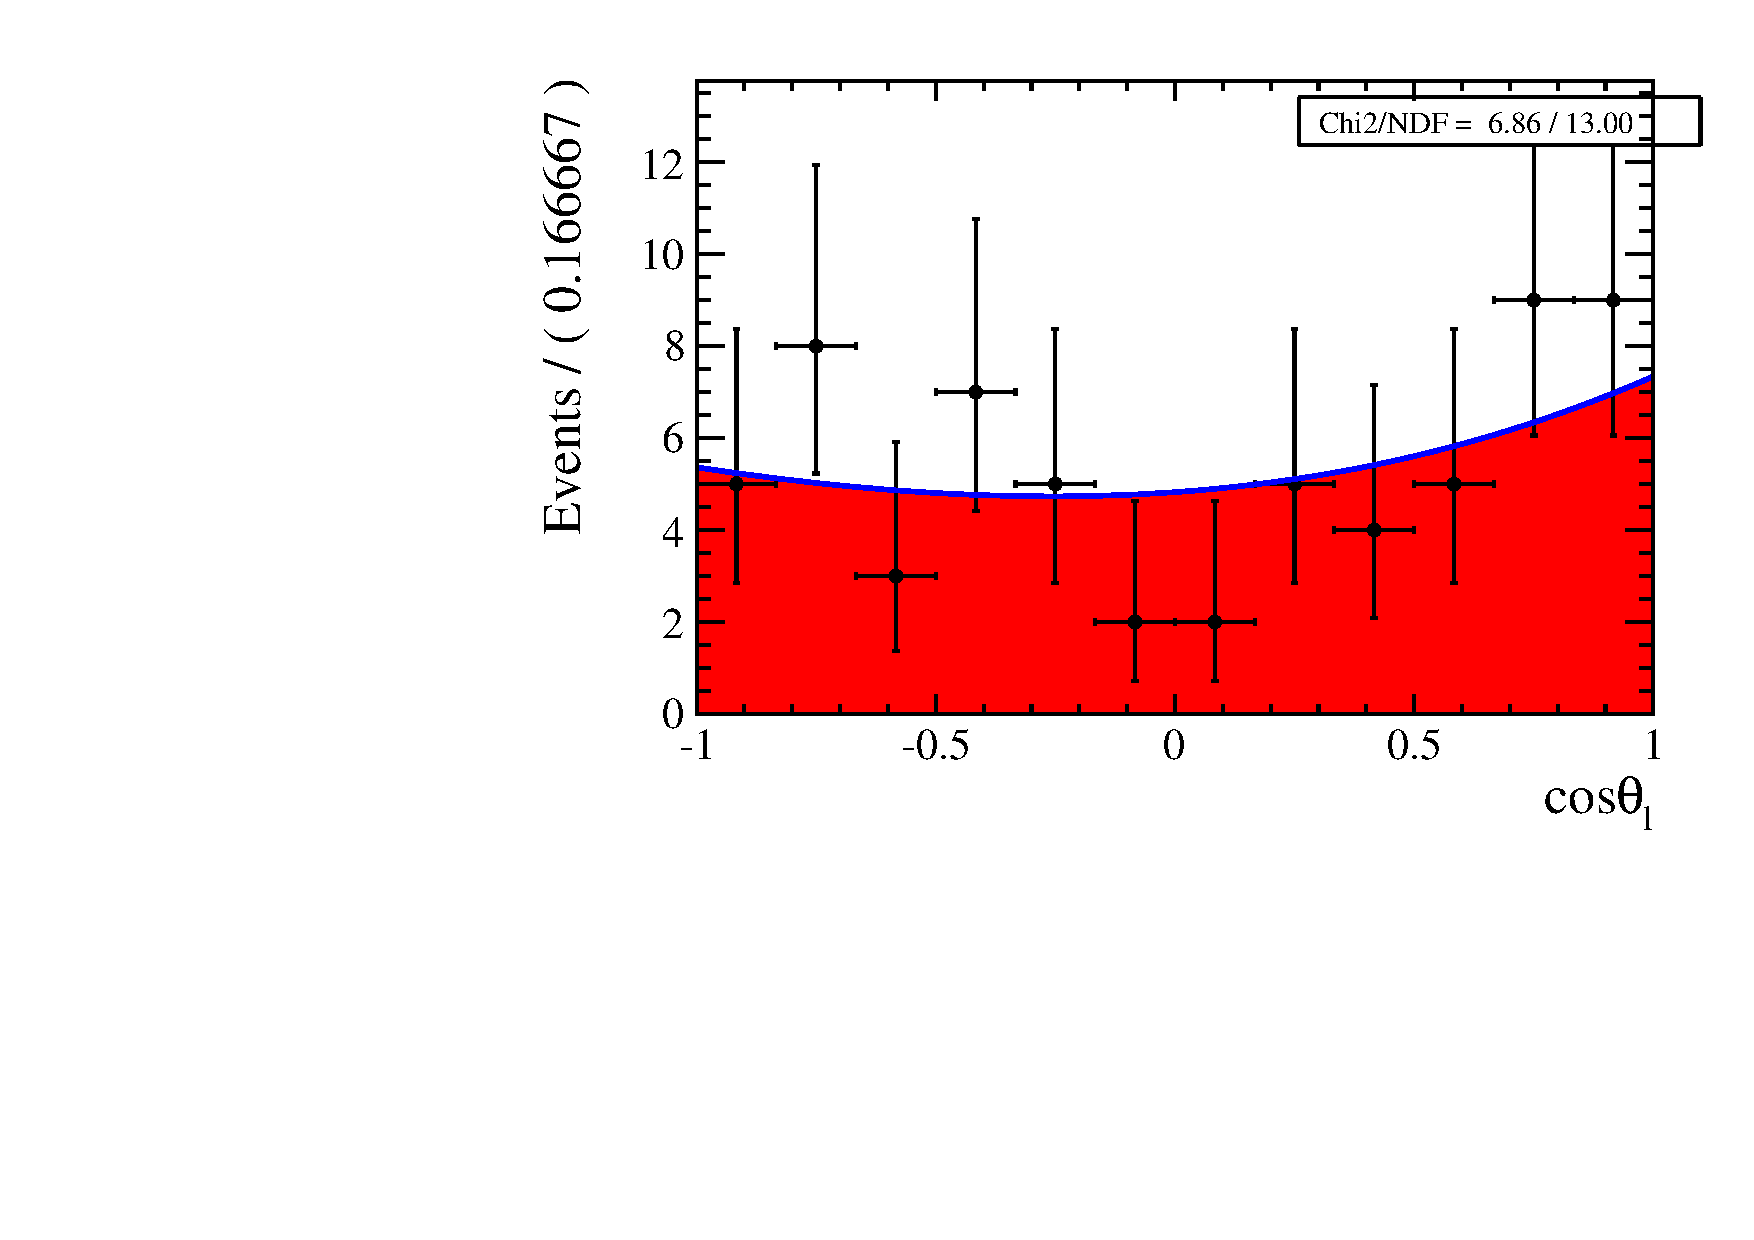
\includegraphics[width=0.40\textwidth]{Lmumu/figs/Side_DD_q2_1500_1600.pdf}
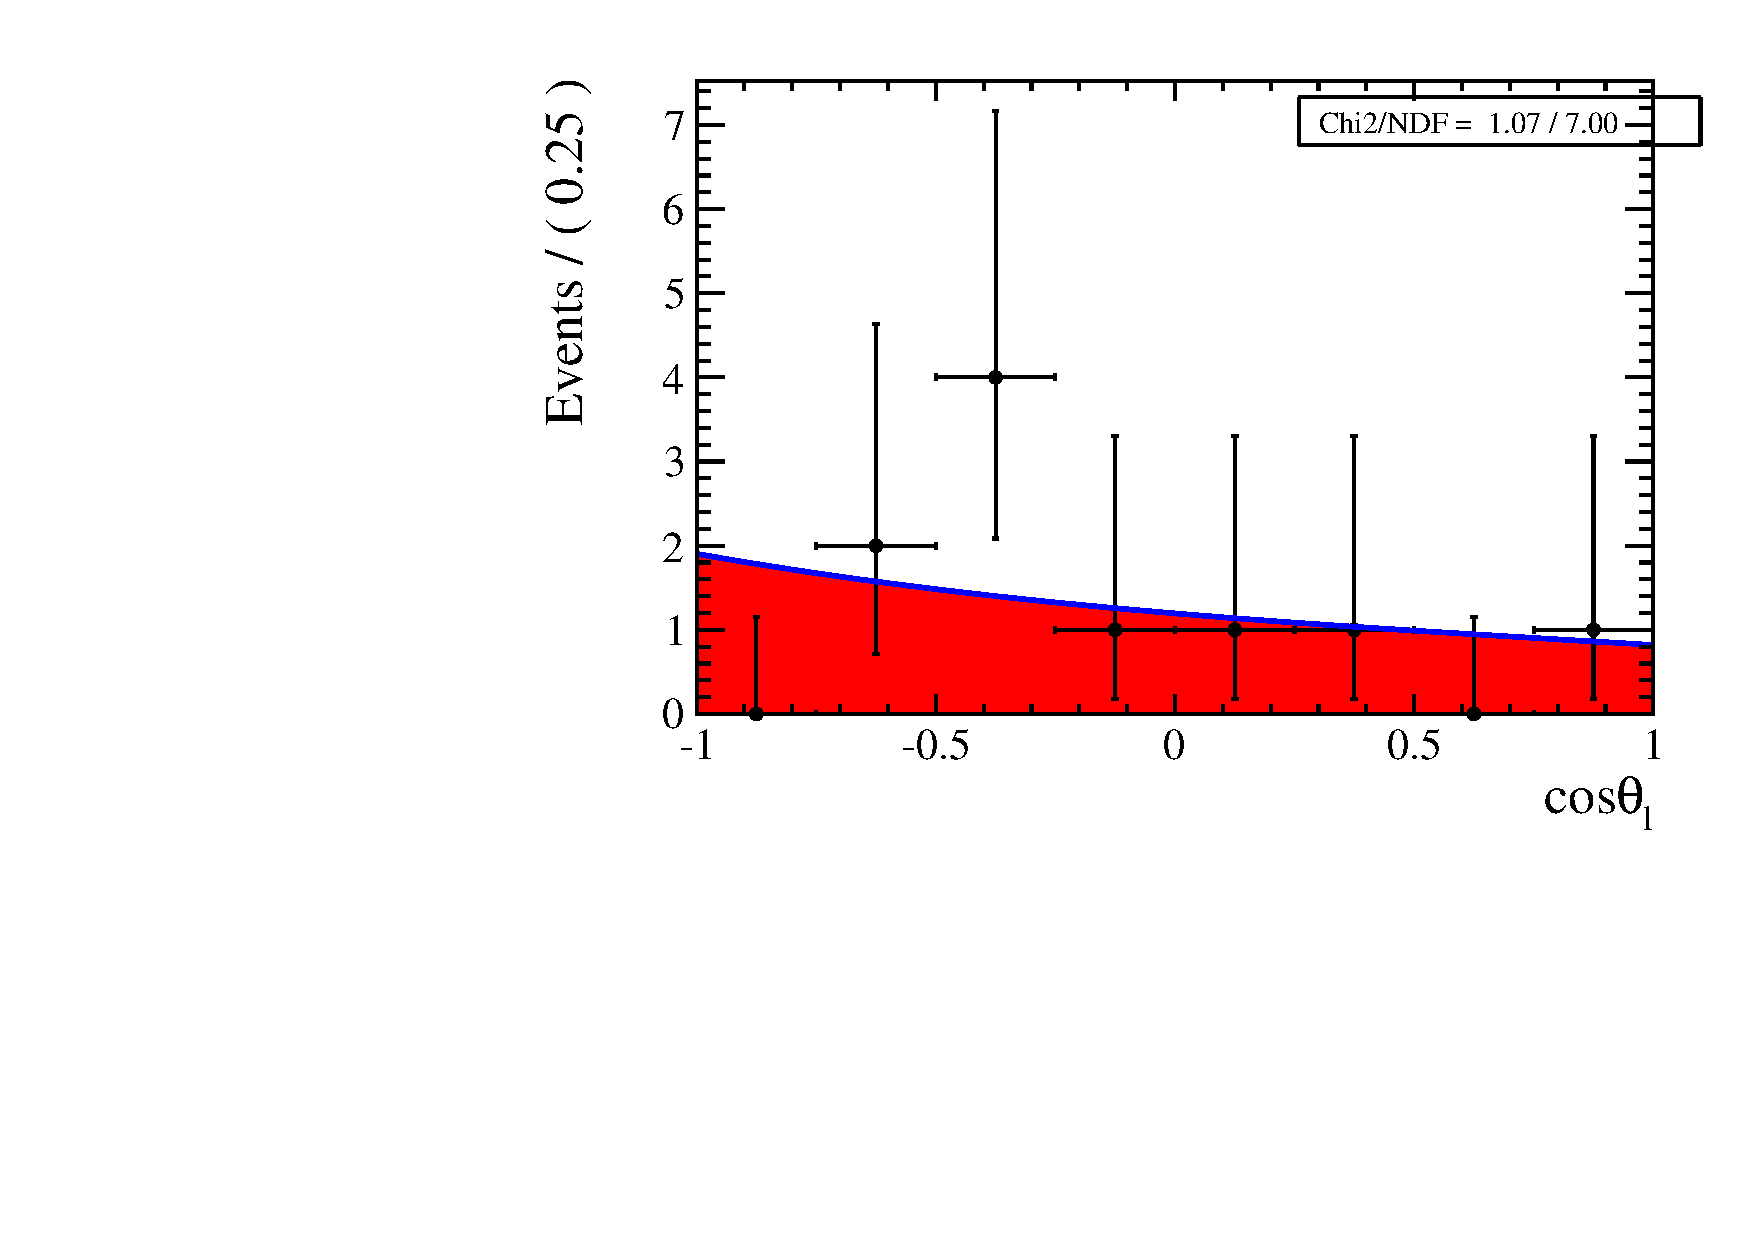
\includegraphics[width=0.40\textwidth]{Lmumu/figs/Side_LL_q2_1500_1600.pdf} \\
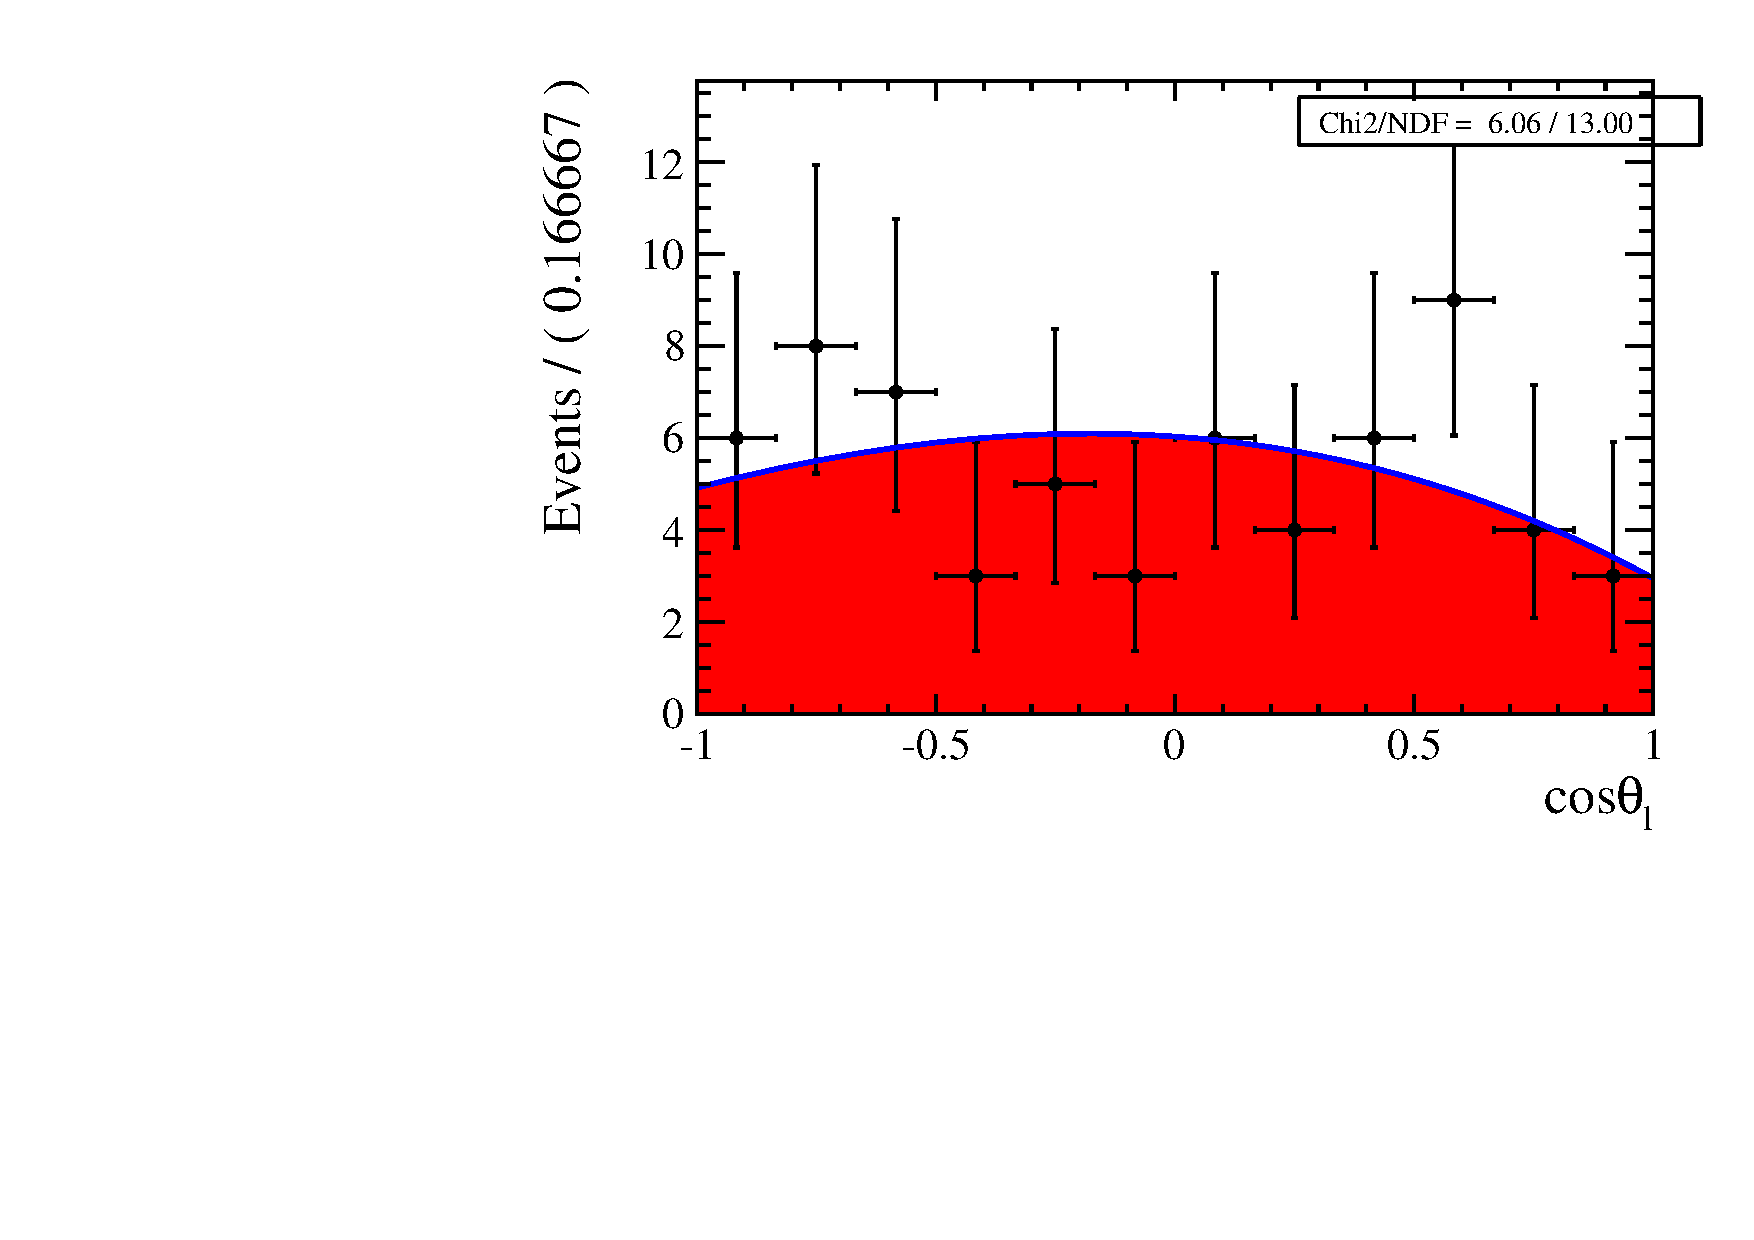
\includegraphics[width=0.40\textwidth]{Lmumu/figs/SideB_DD_q2_1500_1600.pdf}
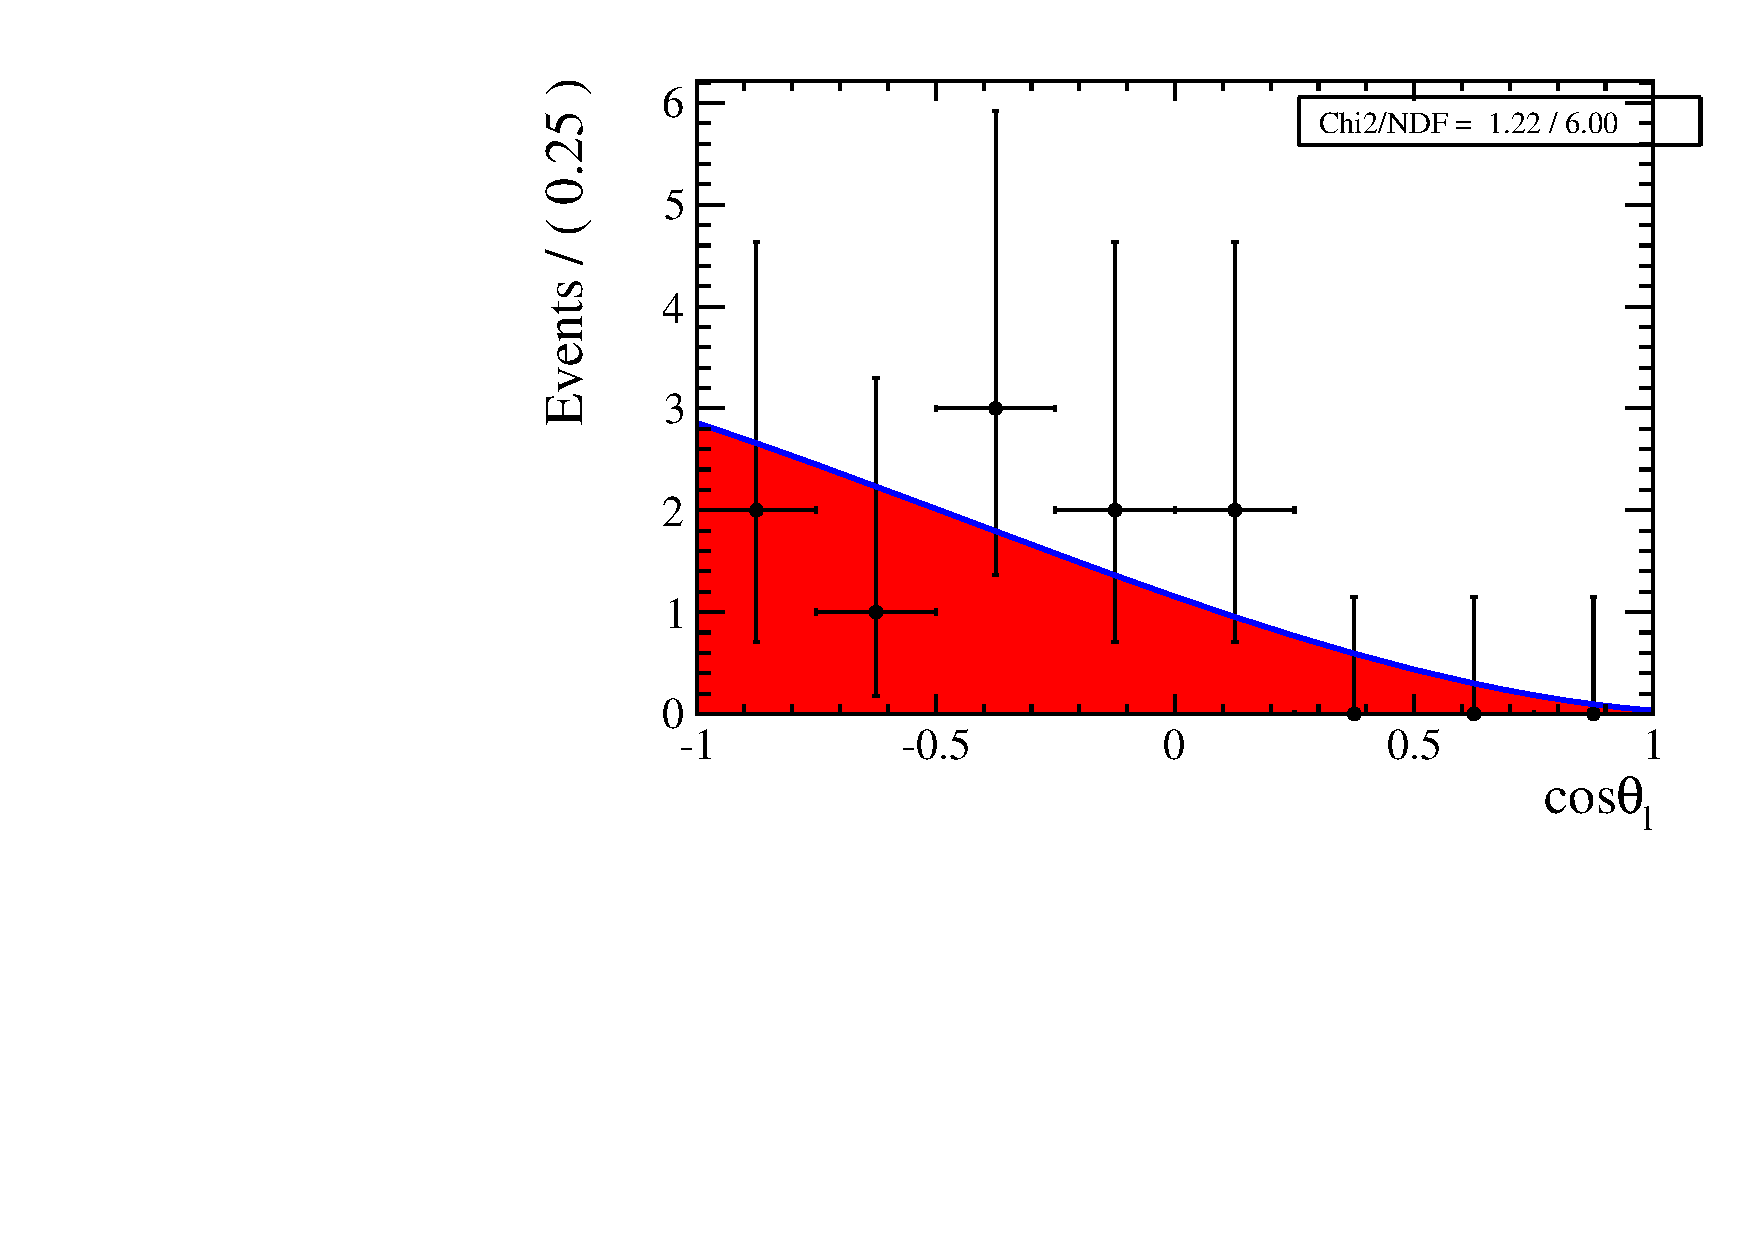
\includegraphics[width=0.40\textwidth]{Lmumu/figs/SideB_LL_q2_1500_1600.pdf}
\caption{Angular distribution in the sideband ($m_{\Lambda\mumu} > 5700 \mevcc$) as a function of $\cos\theta_\Lambda$ (top) and $\cos\theta_\Lambda$ (bottom) for down-down (left) and long-long (right) for events in the $15.0-16.0$GeV^2/c^2$$ \qsq bin.  }
\end{figure}


%%%%%%%%%%%%%%%%%%%%%%%%%%%%%%%%%%%%%%%%%%%%%%%%%%%%%%%%%


\begin{figure}[!htb]
\centering
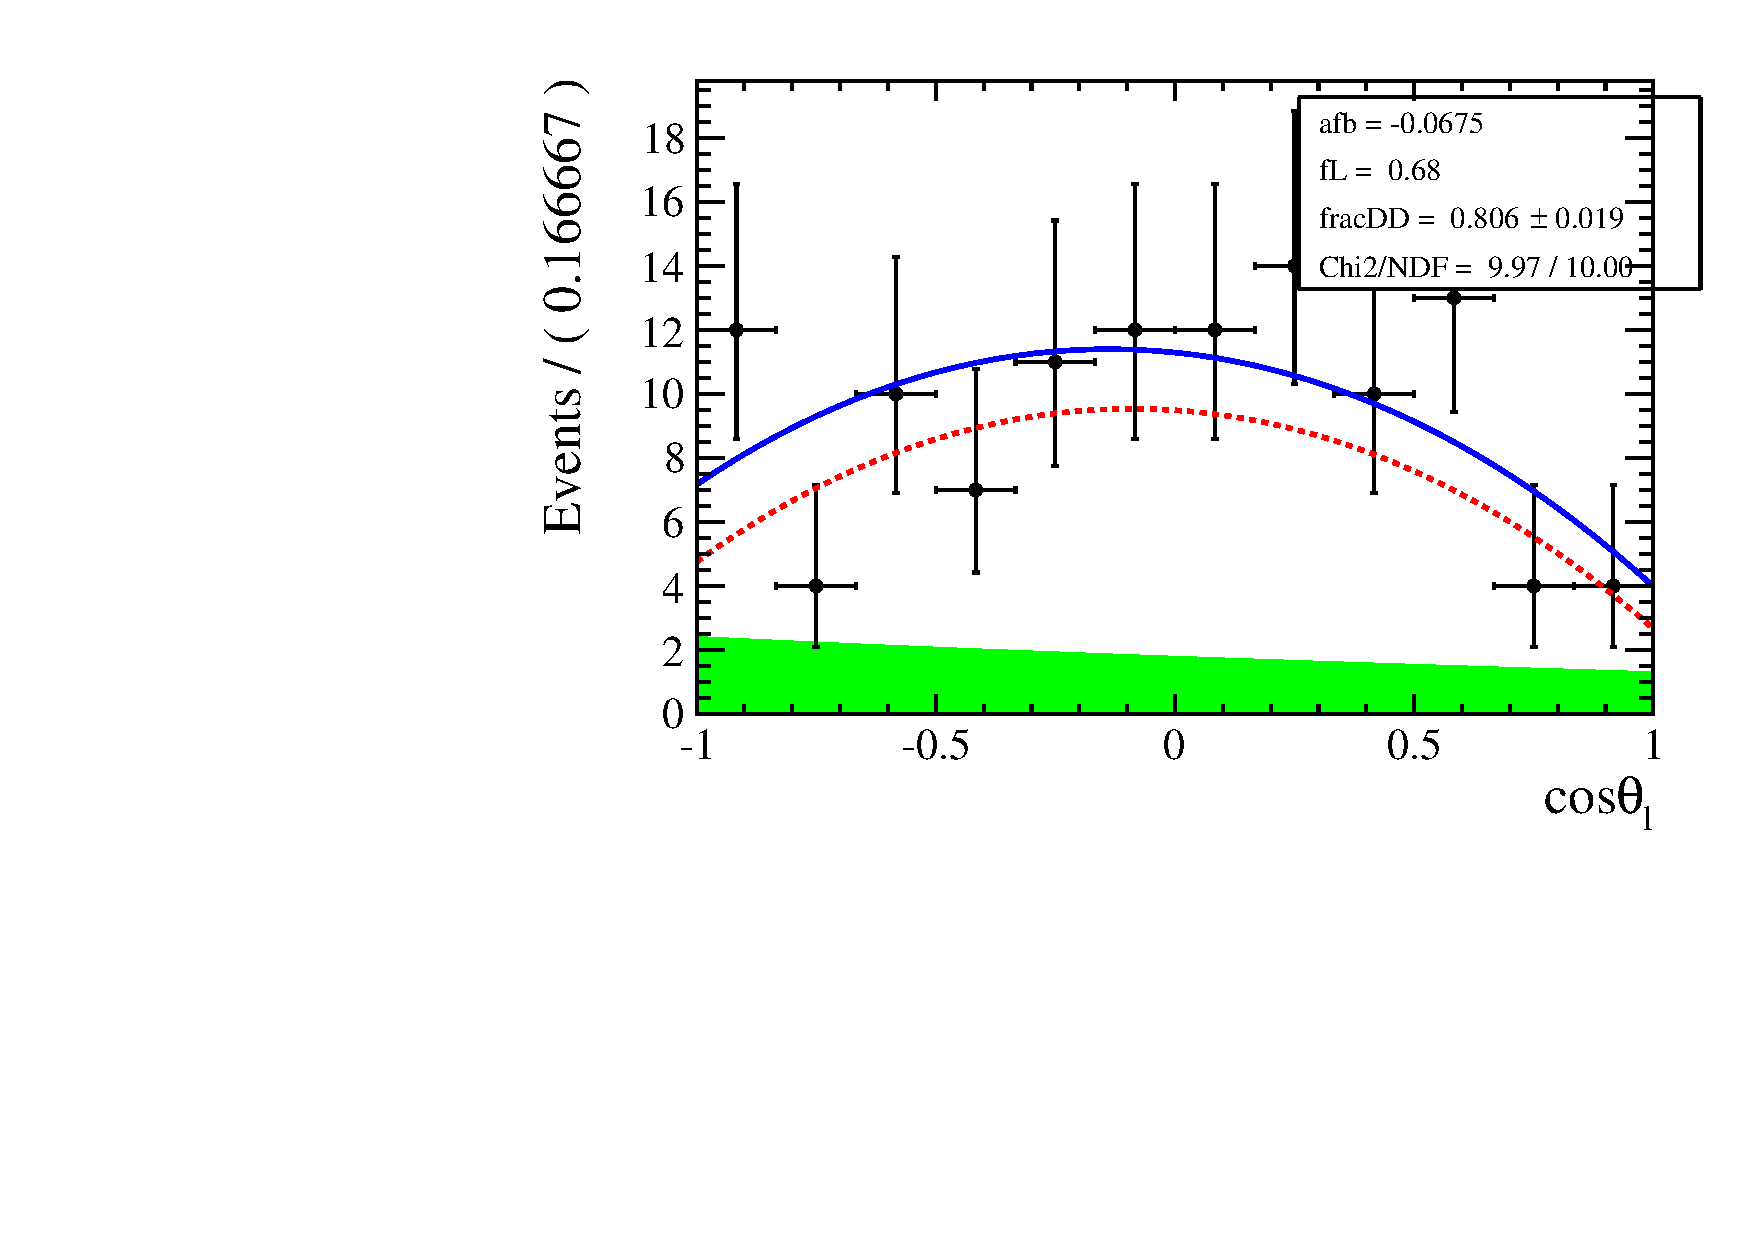
\includegraphics[width=0.40\textwidth]{Lmumu/figs/Afb_DD_q2_1600_1800.pdf}
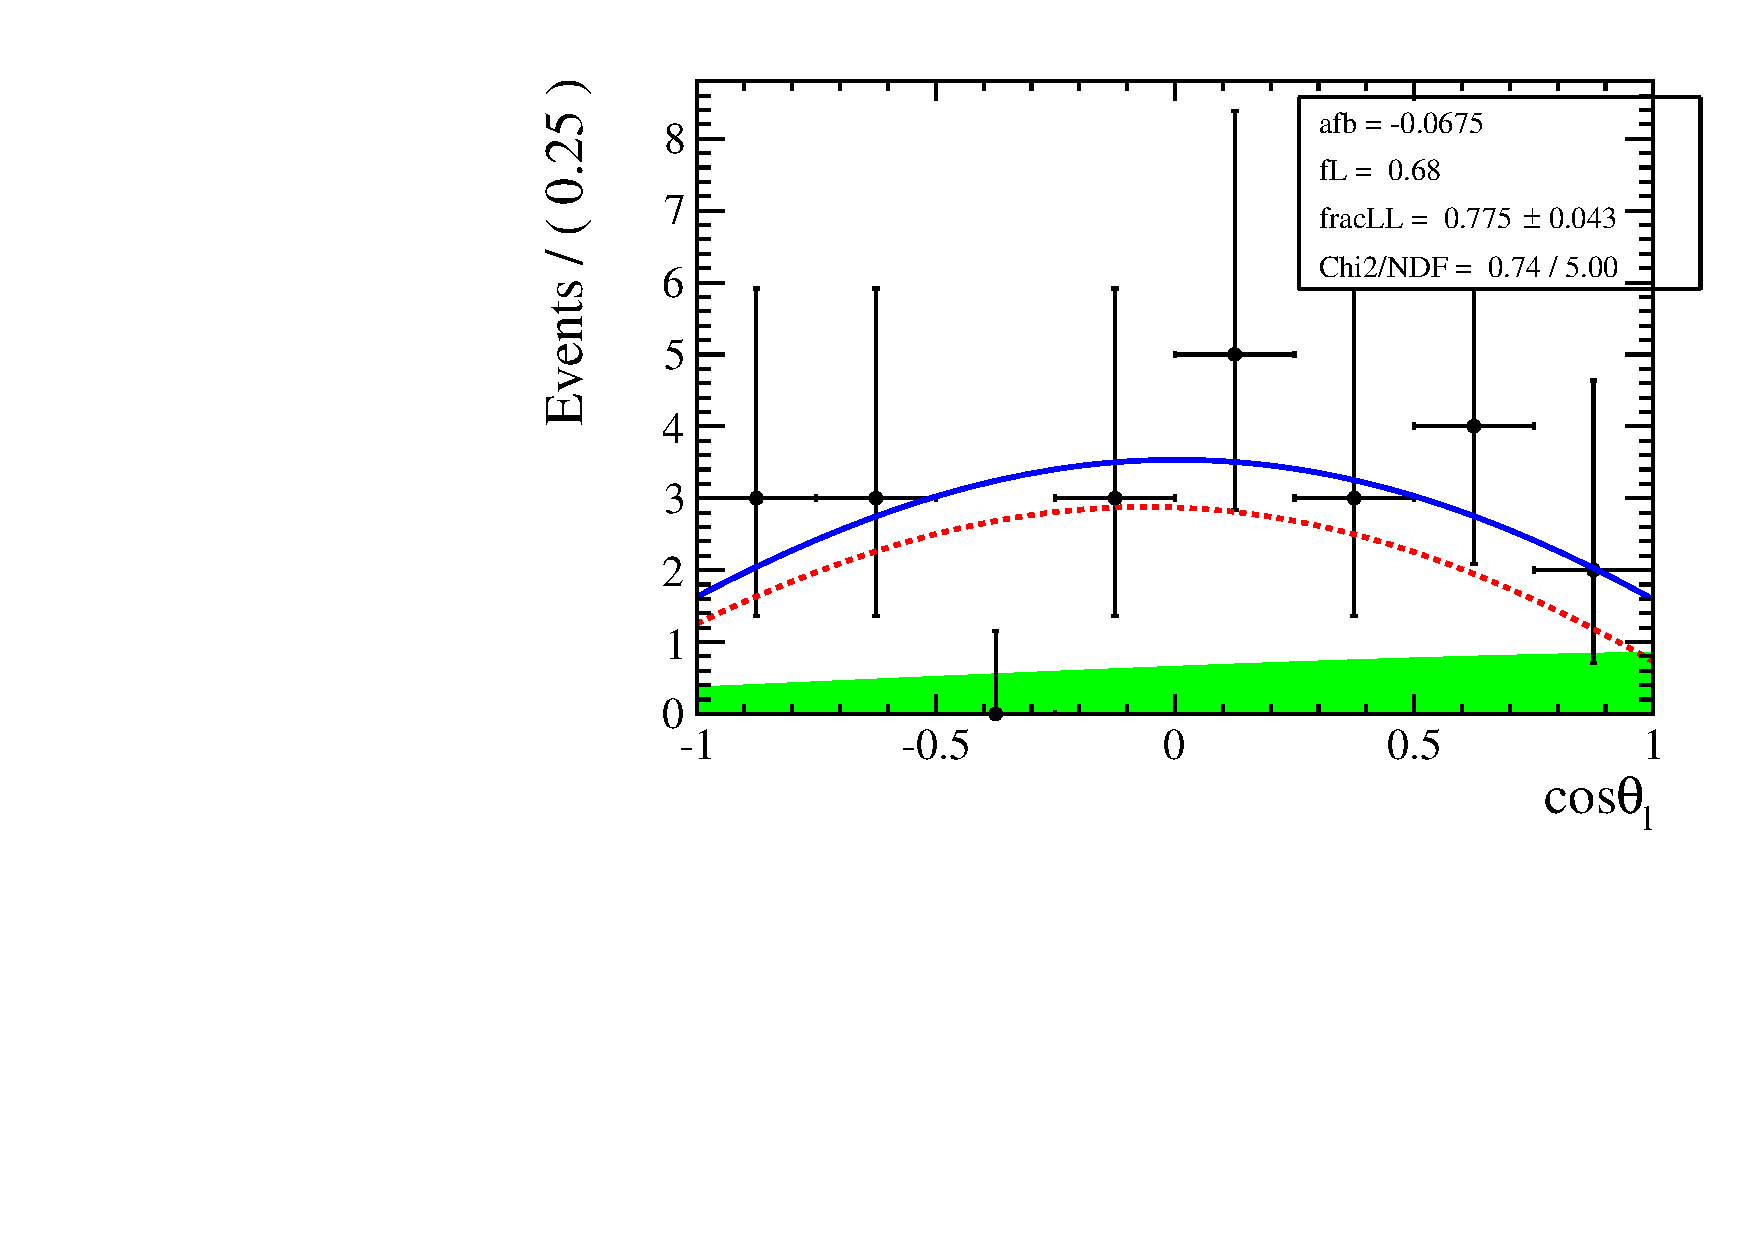
\includegraphics[width=0.40\textwidth]{Lmumu/figs/Afb_LL_q2_1600_1800.pdf} \\
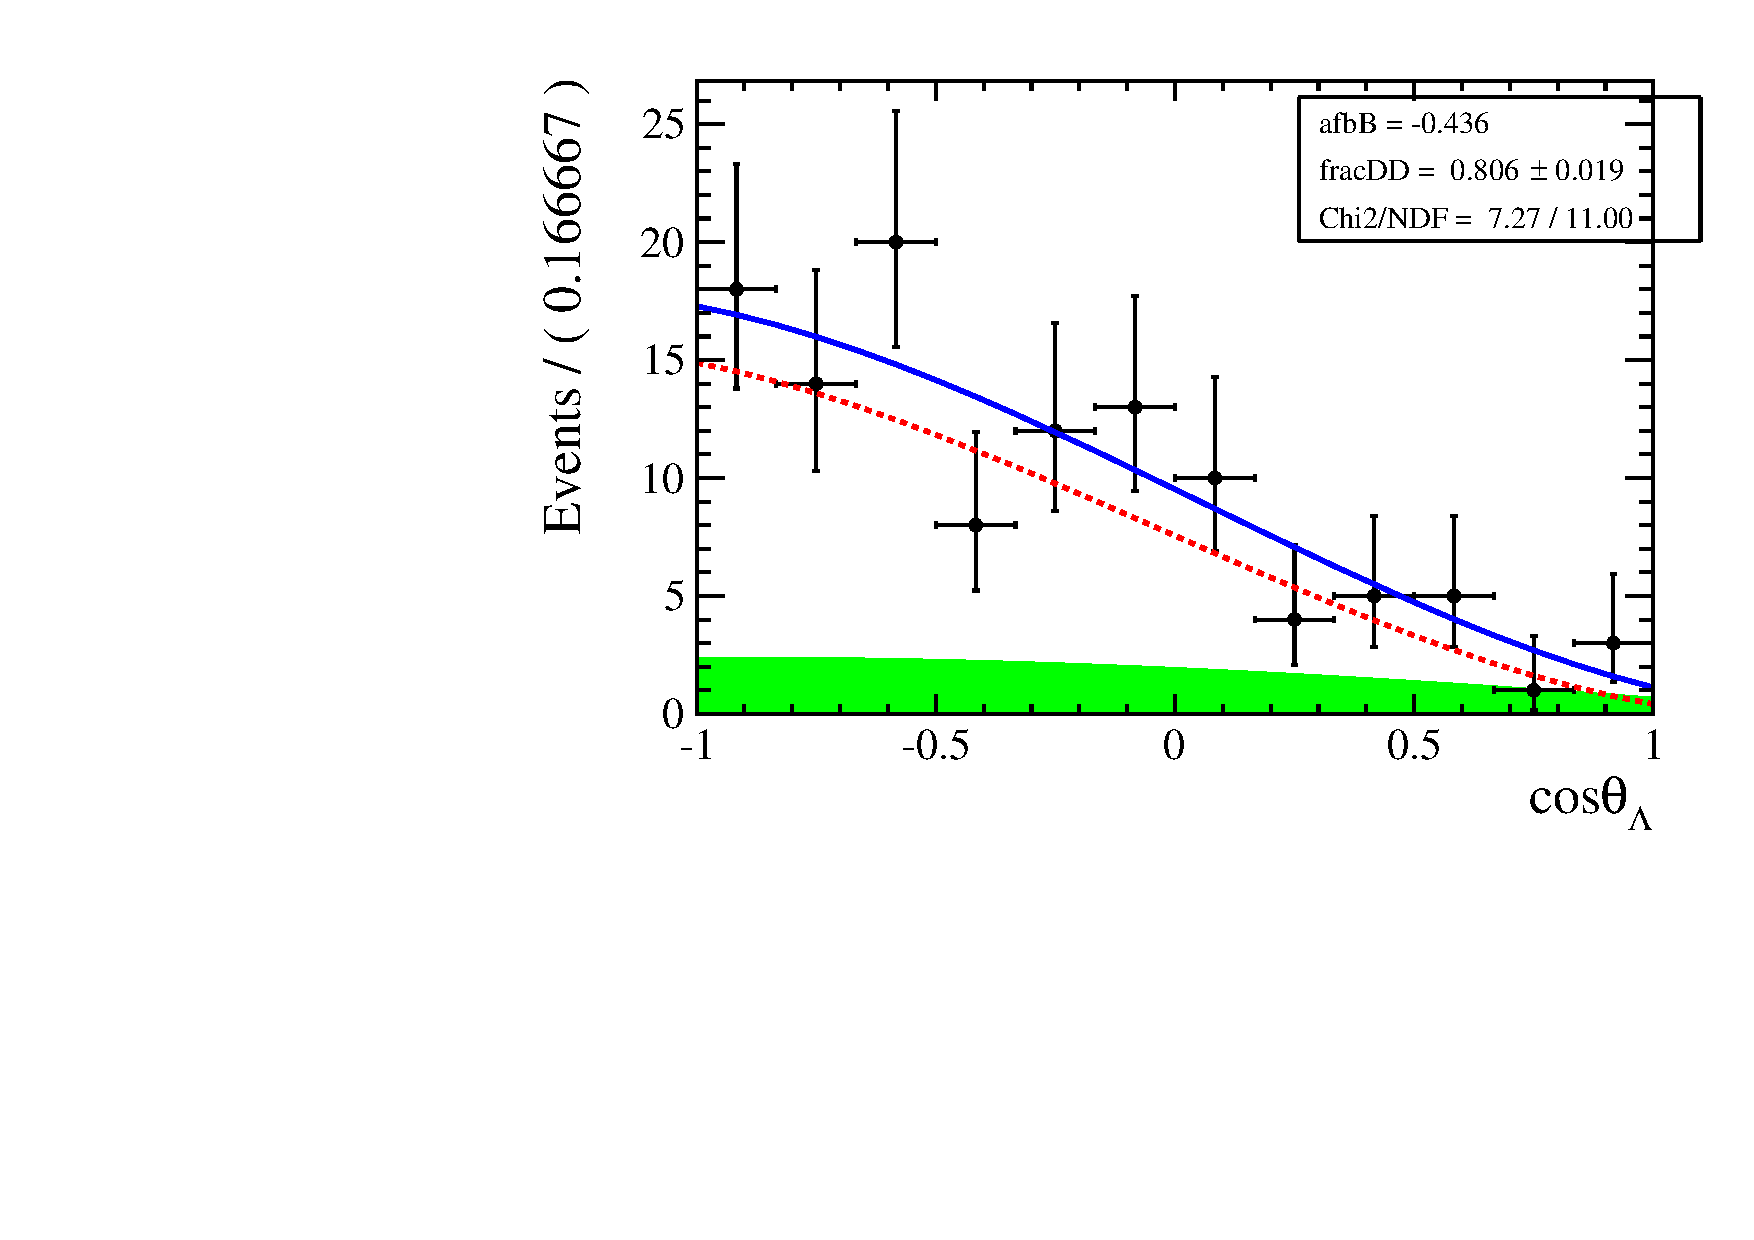
\includegraphics[width=0.40\textwidth]{Lmumu/figs/AfbB_DD_q2_1600_1800.pdf}
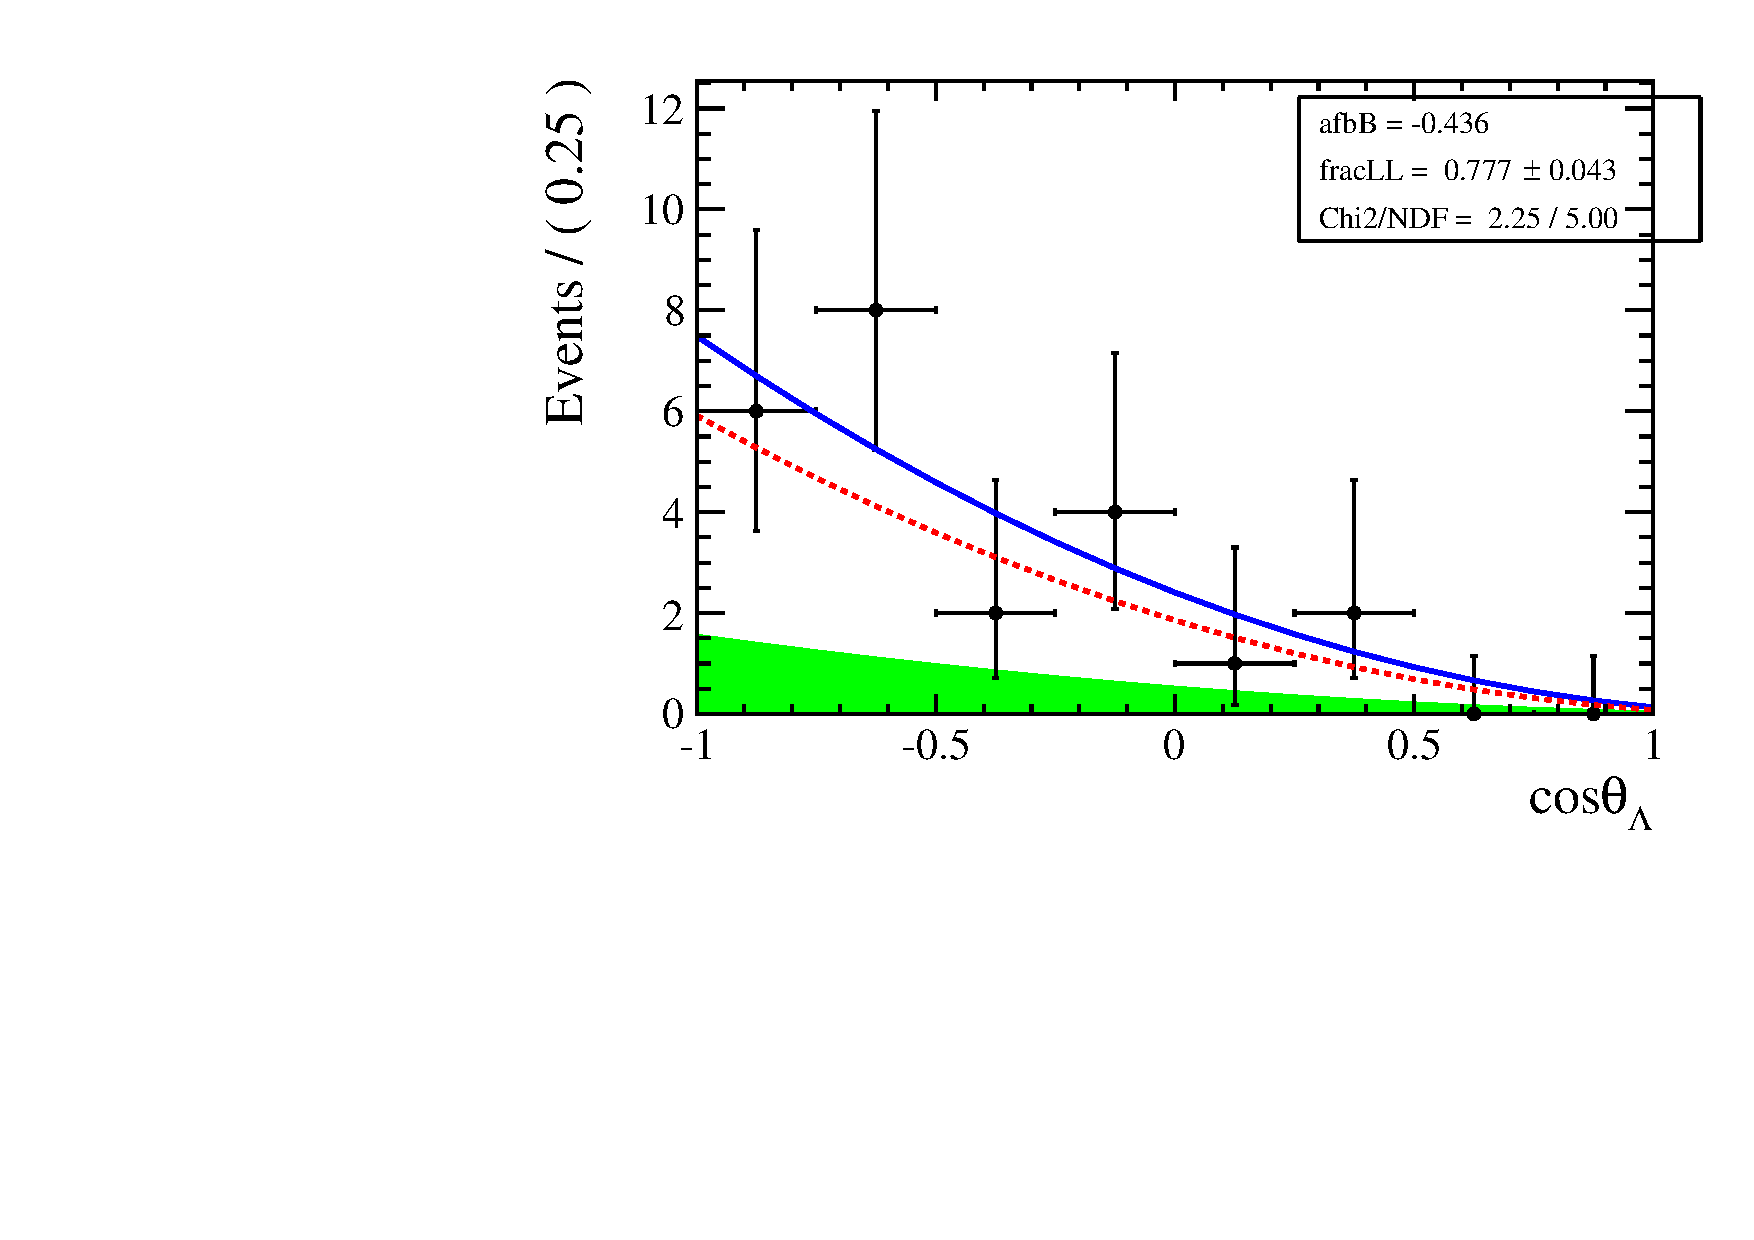
\includegraphics[width=0.40\textwidth]{Lmumu/figs/AfbB_LL_q2_1600_1800.pdf}
\caption{Fitted angular distribution as a function of $\cos\theta_\ell$ (top) and $\cos\theta_\Lambda$ (bottom) for down-down (left) and long-long (right) for events in the $16.0-18.0$GeV^2/c^2$$ \qsq bin.  }
\end{figure}


\begin{figure}[!htb]
\centering
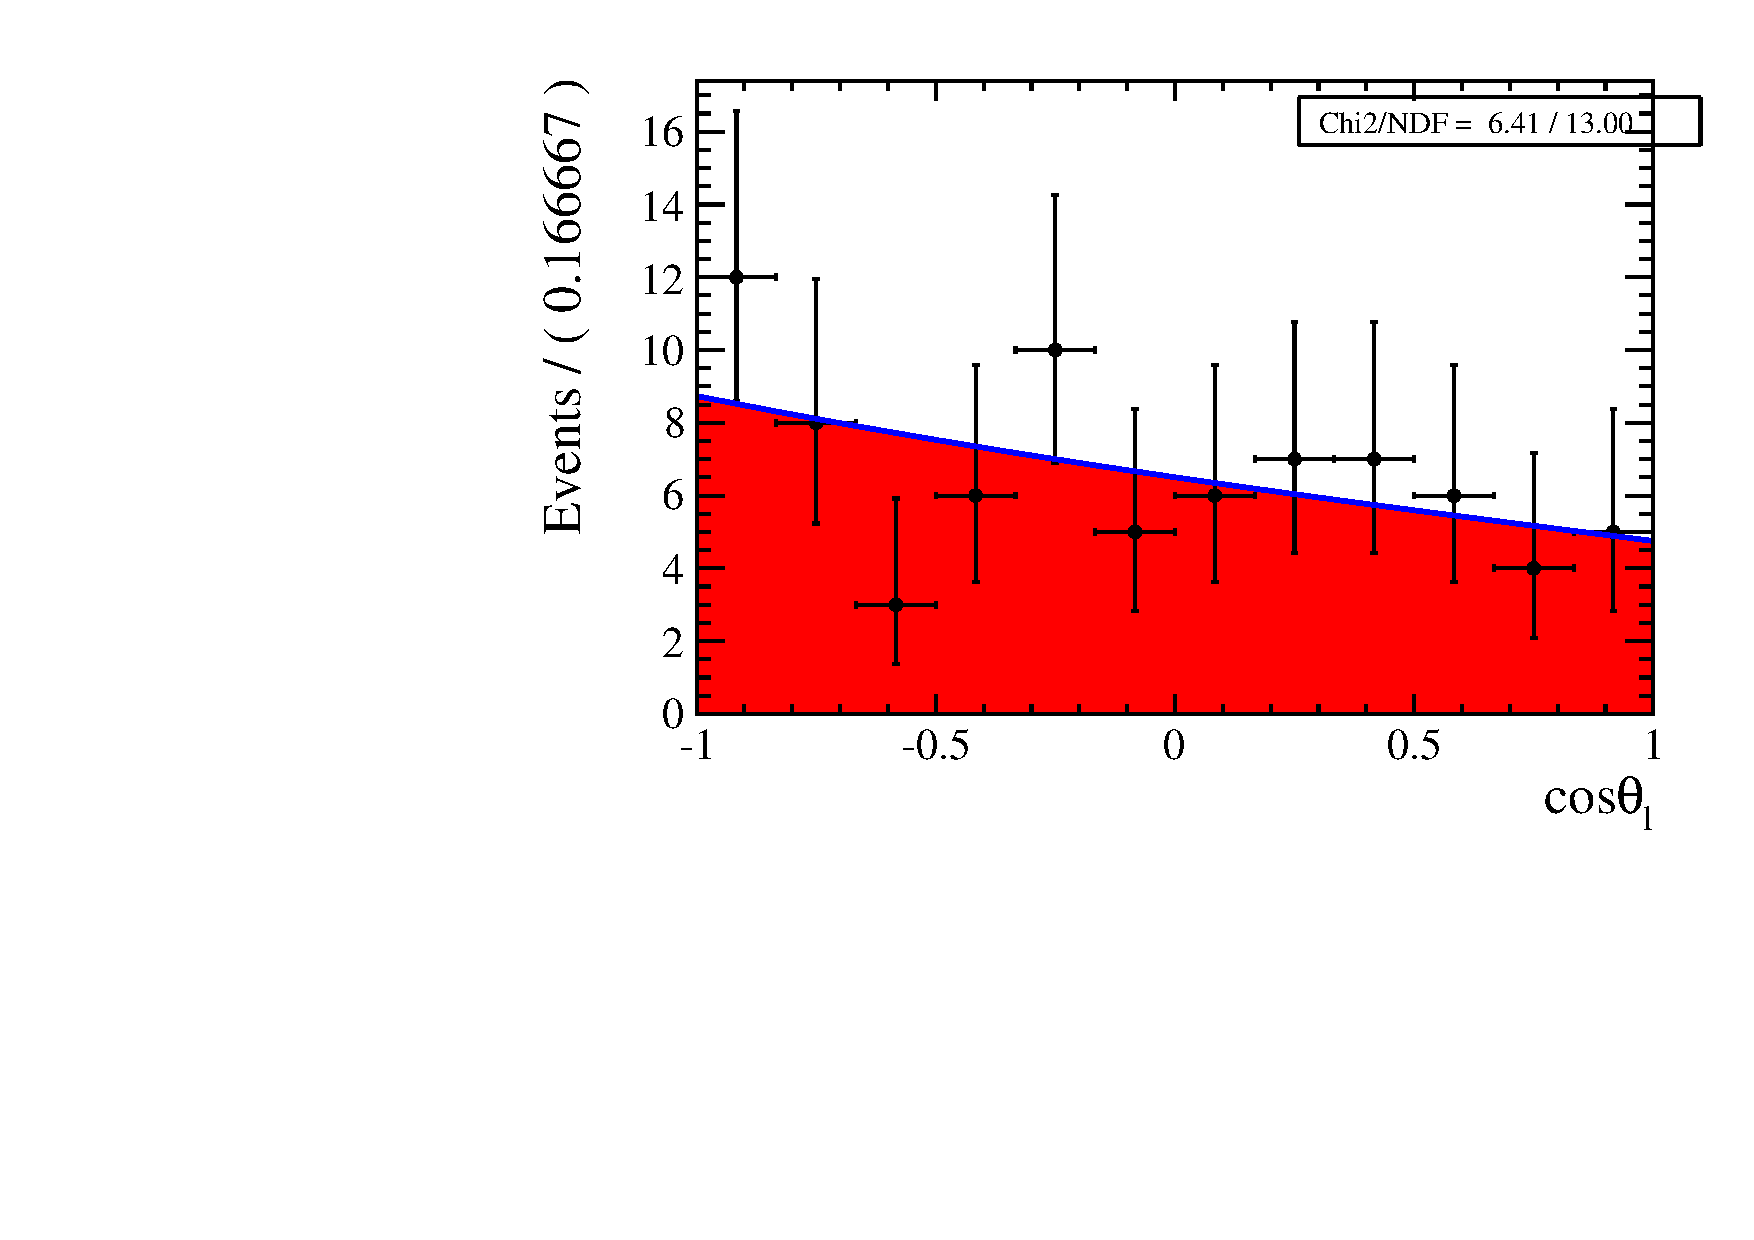
\includegraphics[width=0.40\textwidth]{Lmumu/figs/Side_DD_q2_1600_1800.pdf}
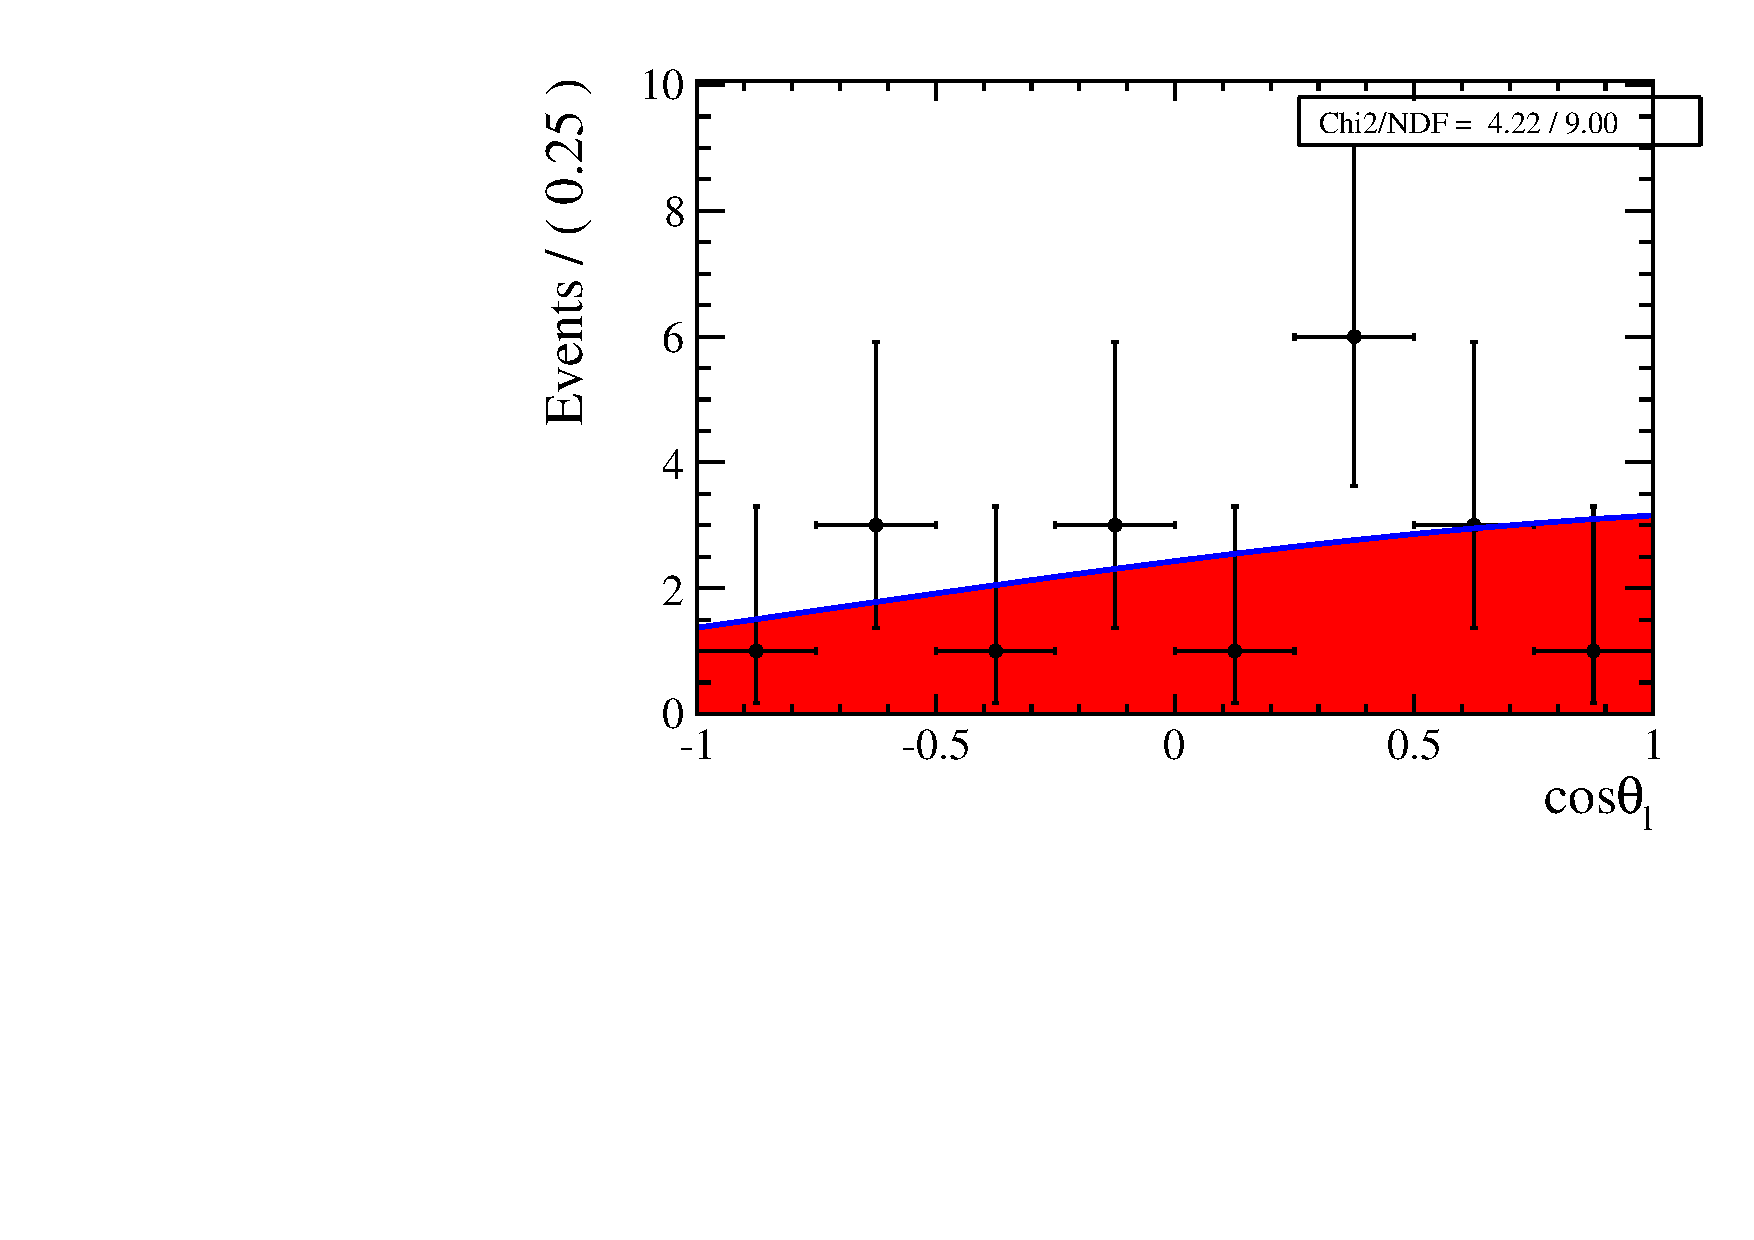
\includegraphics[width=0.40\textwidth]{Lmumu/figs/Side_LL_q2_1600_1800.pdf} \\
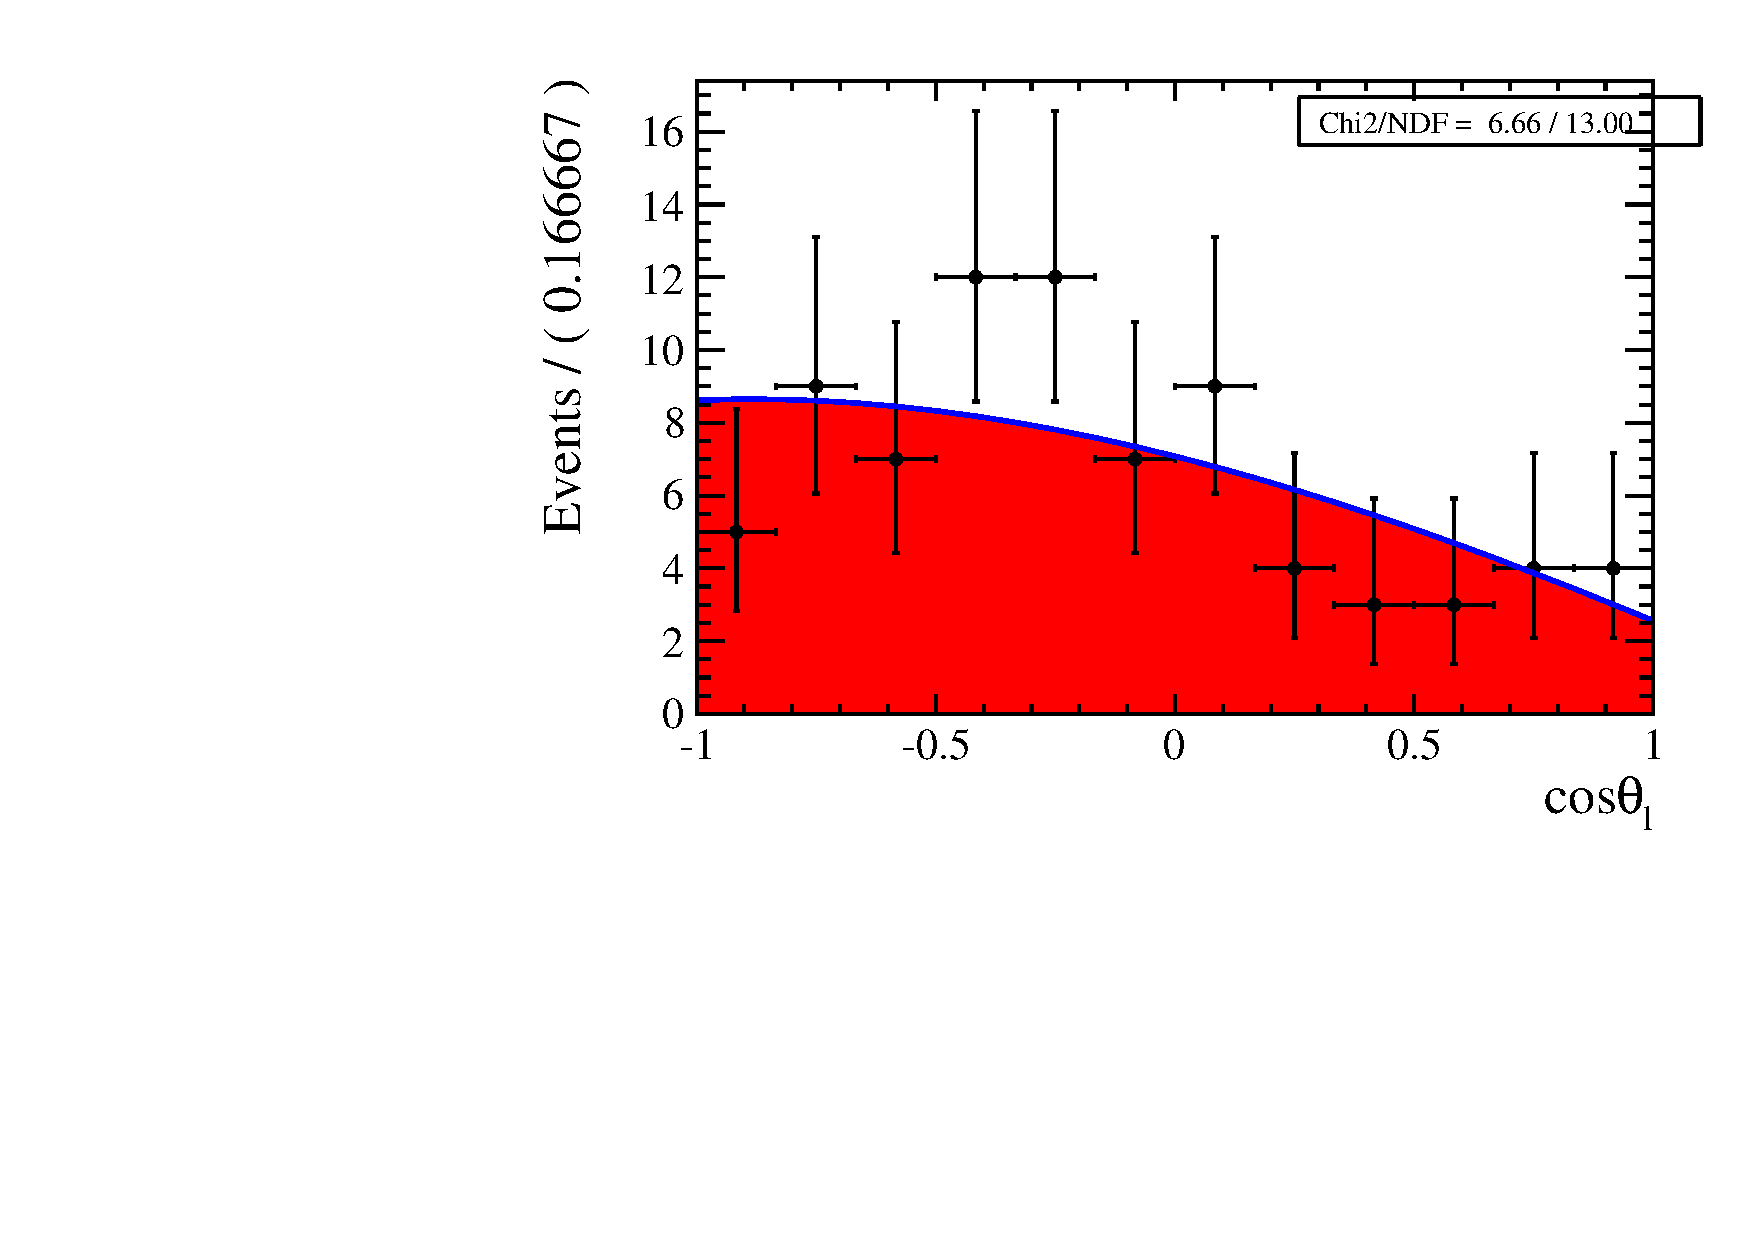
\includegraphics[width=0.40\textwidth]{Lmumu/figs/SideB_DD_q2_1600_1800.pdf}
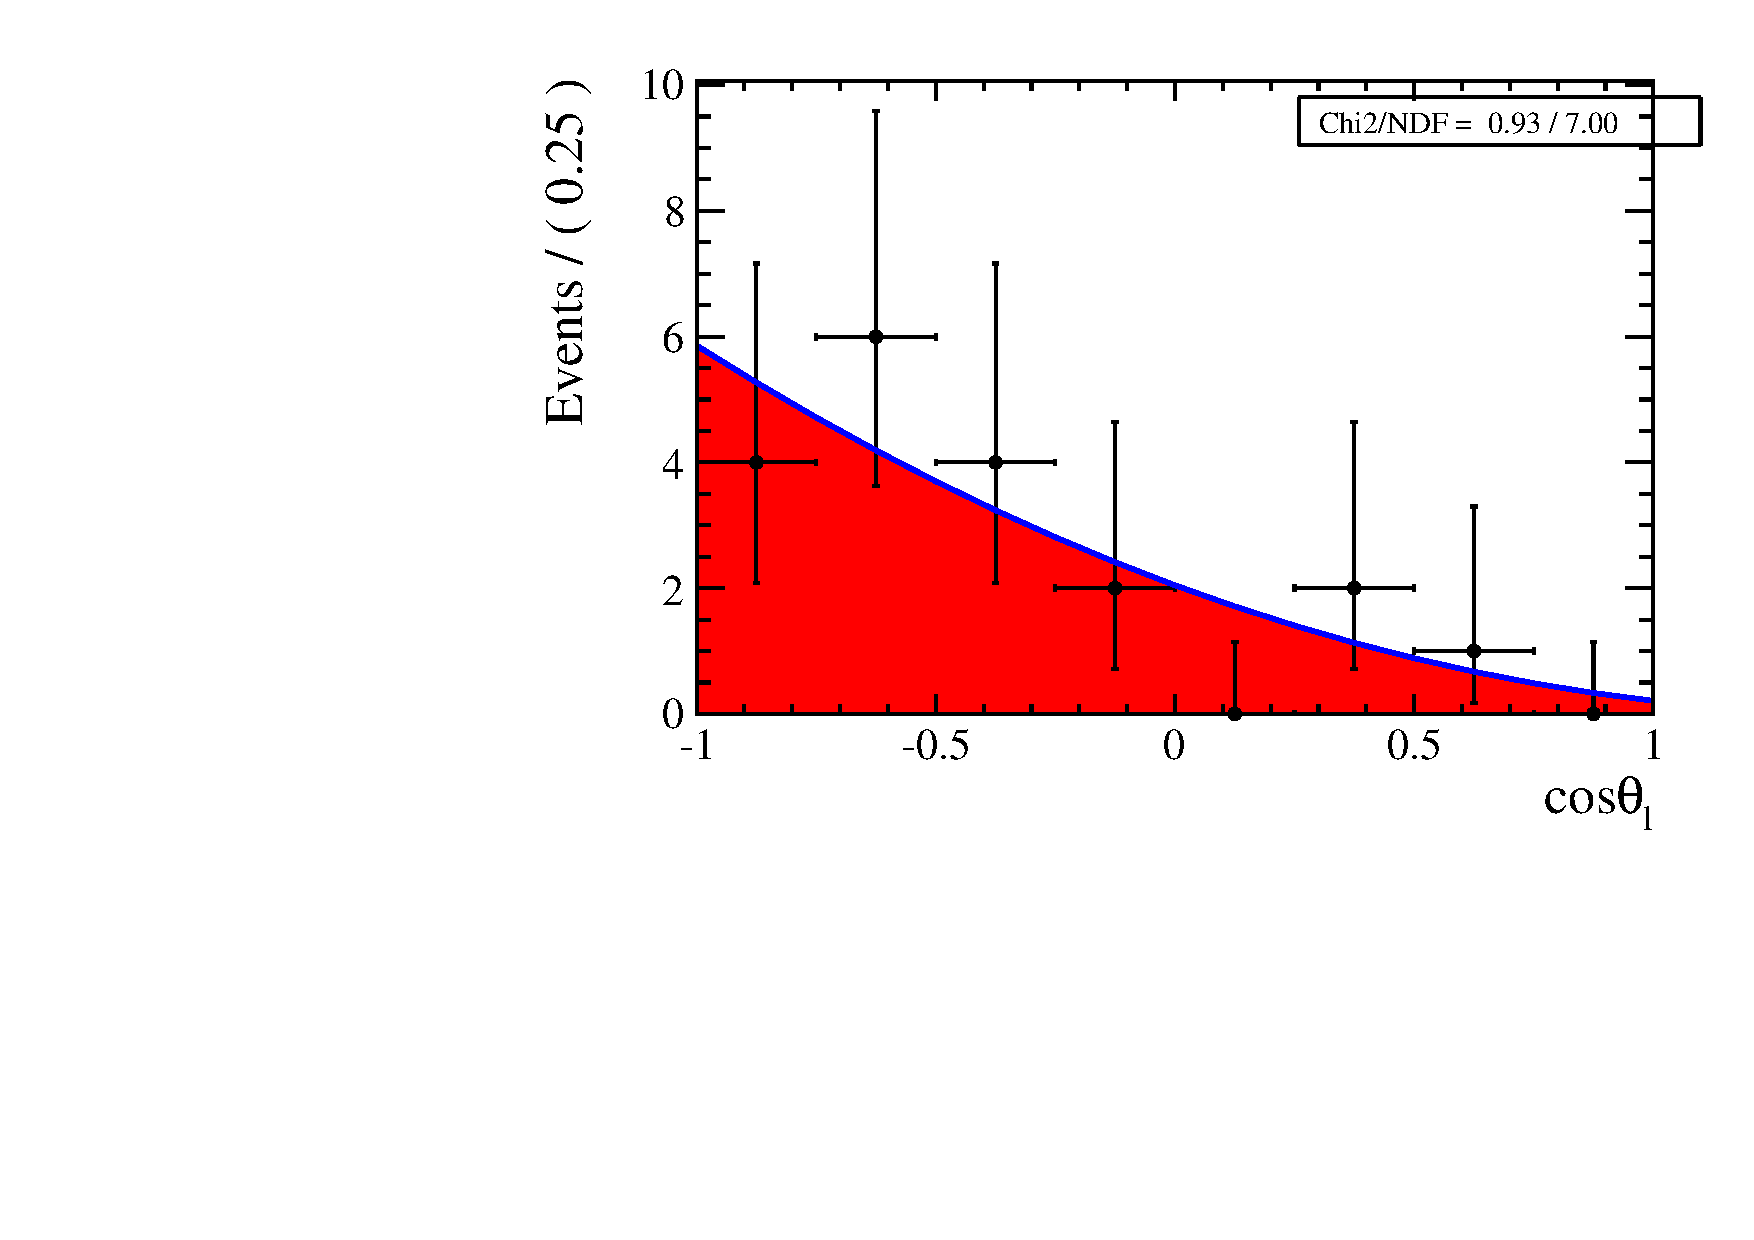
\includegraphics[width=0.40\textwidth]{Lmumu/figs/SideB_LL_q2_1600_1800.pdf}
\caption{Angular distribution in the sideband ($m_{\Lambda\mumu} > 5700 \mevcc$) as a function of $\cos\theta_\Lambda$ (top) and $\cos\theta_\Lambda$ (bottom) for down-down (left) and long-long (right) for events in the $16.0-18.0$GeV^2/c^2$$ \qsq bin.  }
\end{figure}


%%%%%%%%%%%%%%%%%%%%%%%%%%%%%%%%%%%%%%%%%%%%%%%%%%%%%%%%%%%%



\begin{figure}[!htb]
\centering
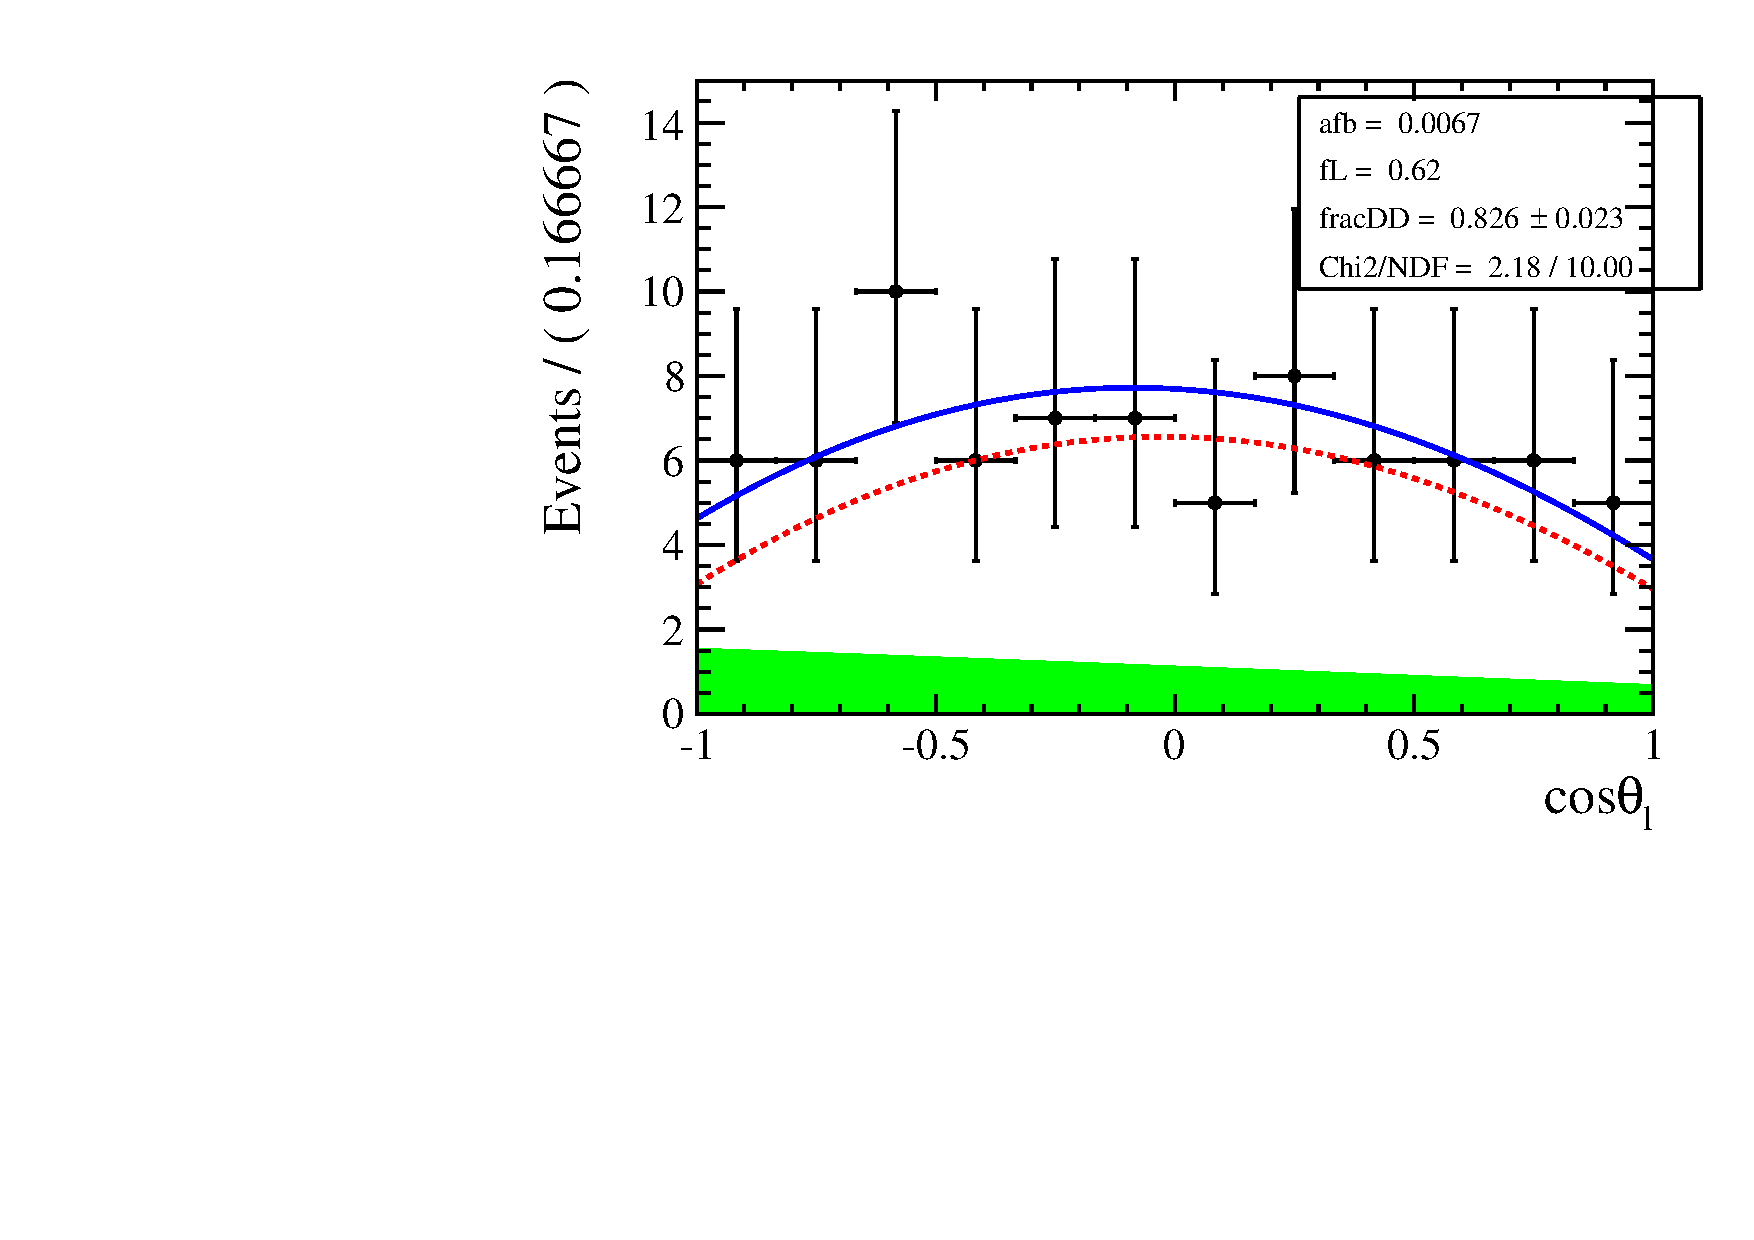
\includegraphics[width=0.40\textwidth]{Lmumu/figs/Afb_DD_q2_1800_2000.pdf}
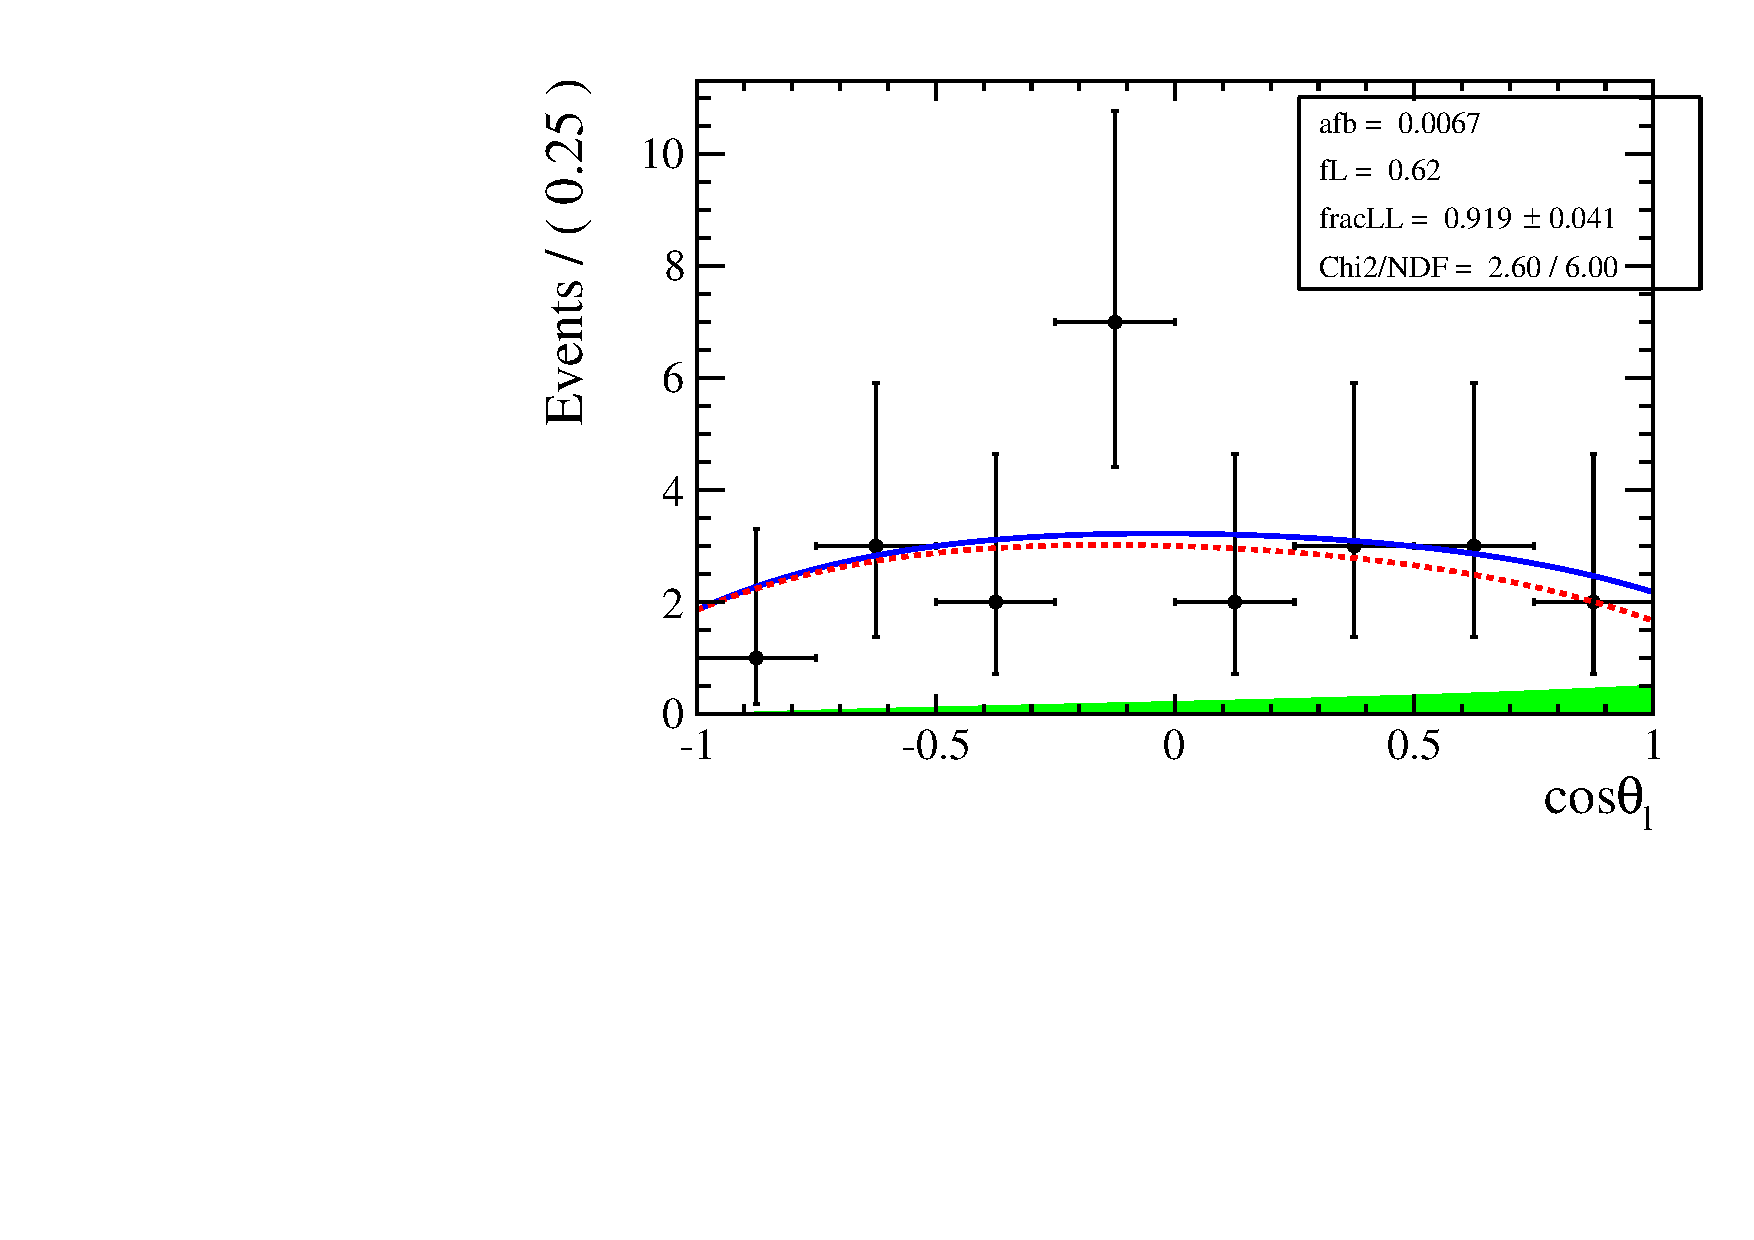
\includegraphics[width=0.40\textwidth]{Lmumu/figs/Afb_LL_q2_1800_2000.pdf} \\
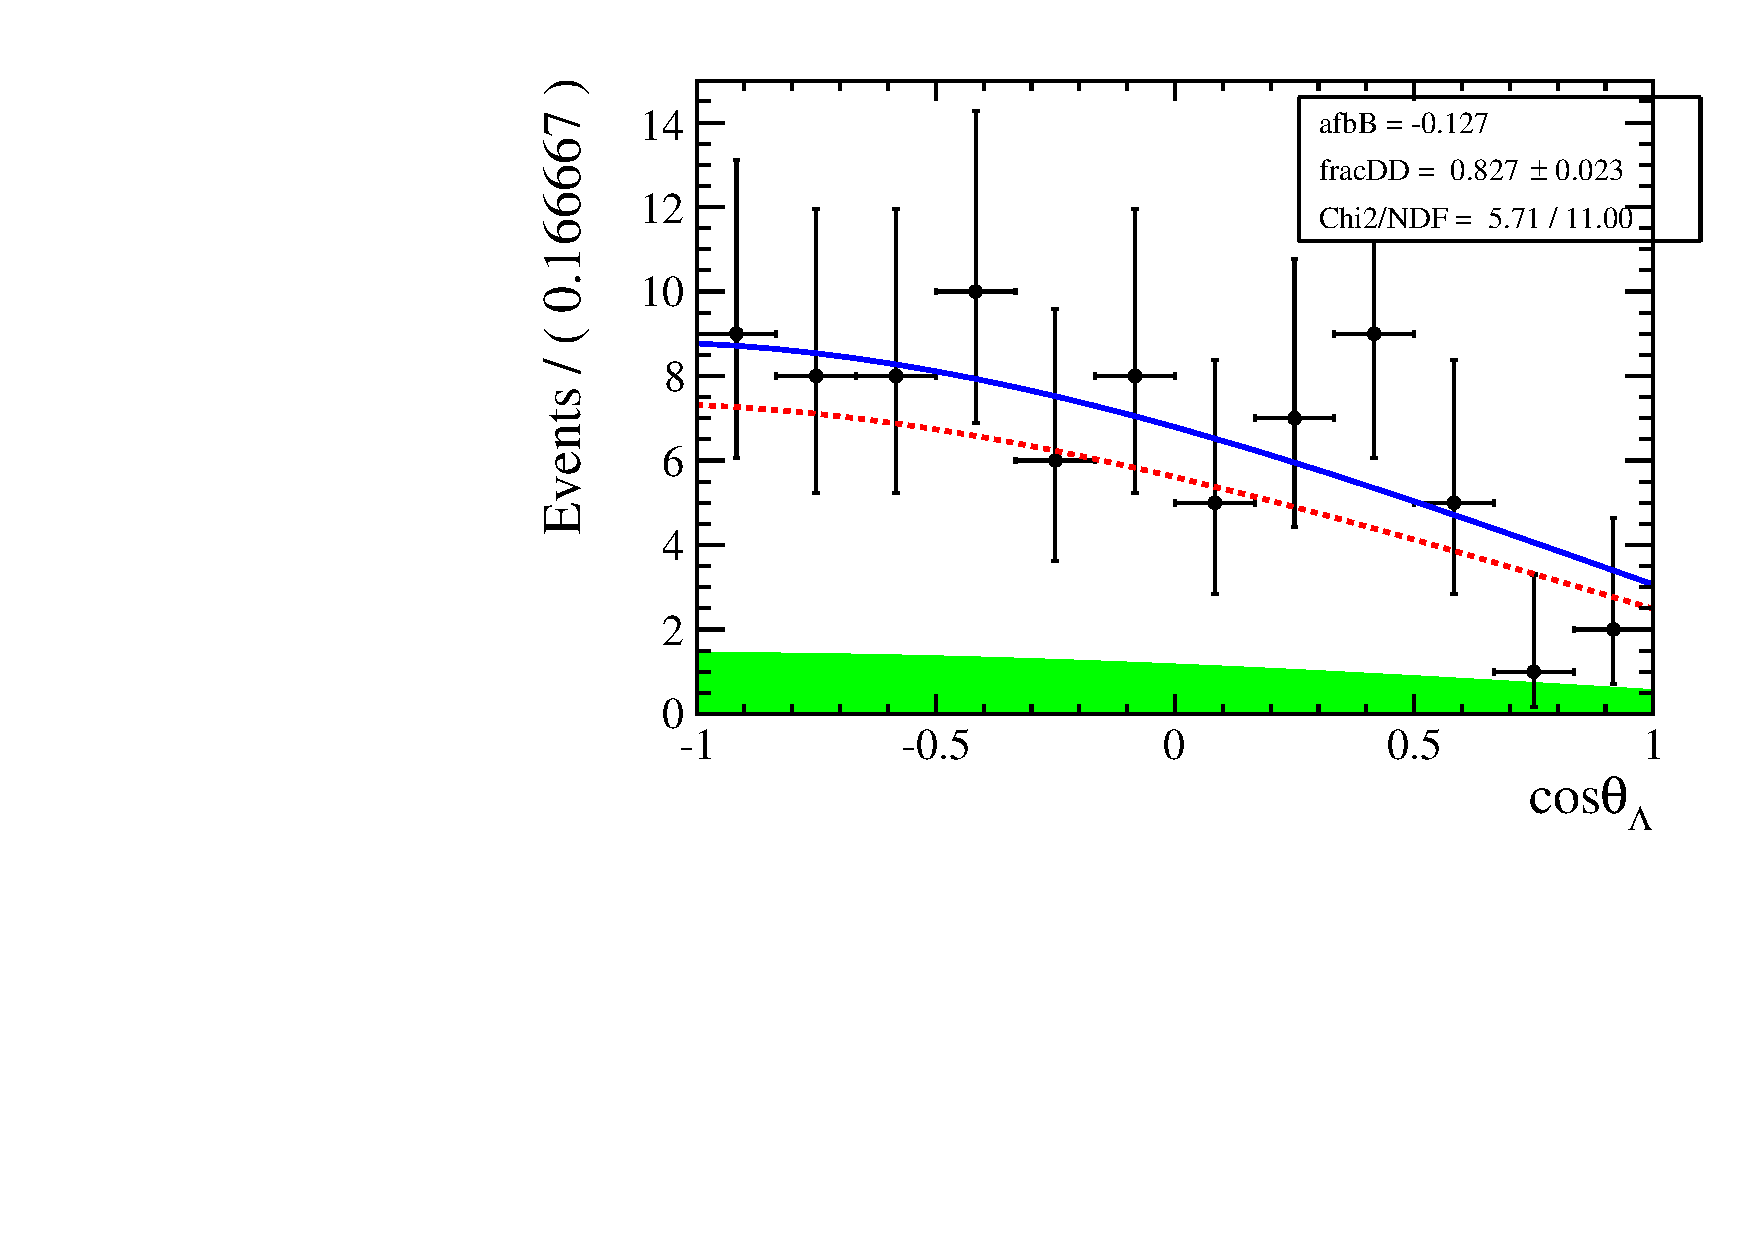
\includegraphics[width=0.40\textwidth]{Lmumu/figs/AfbB_DD_q2_1800_2000.pdf}
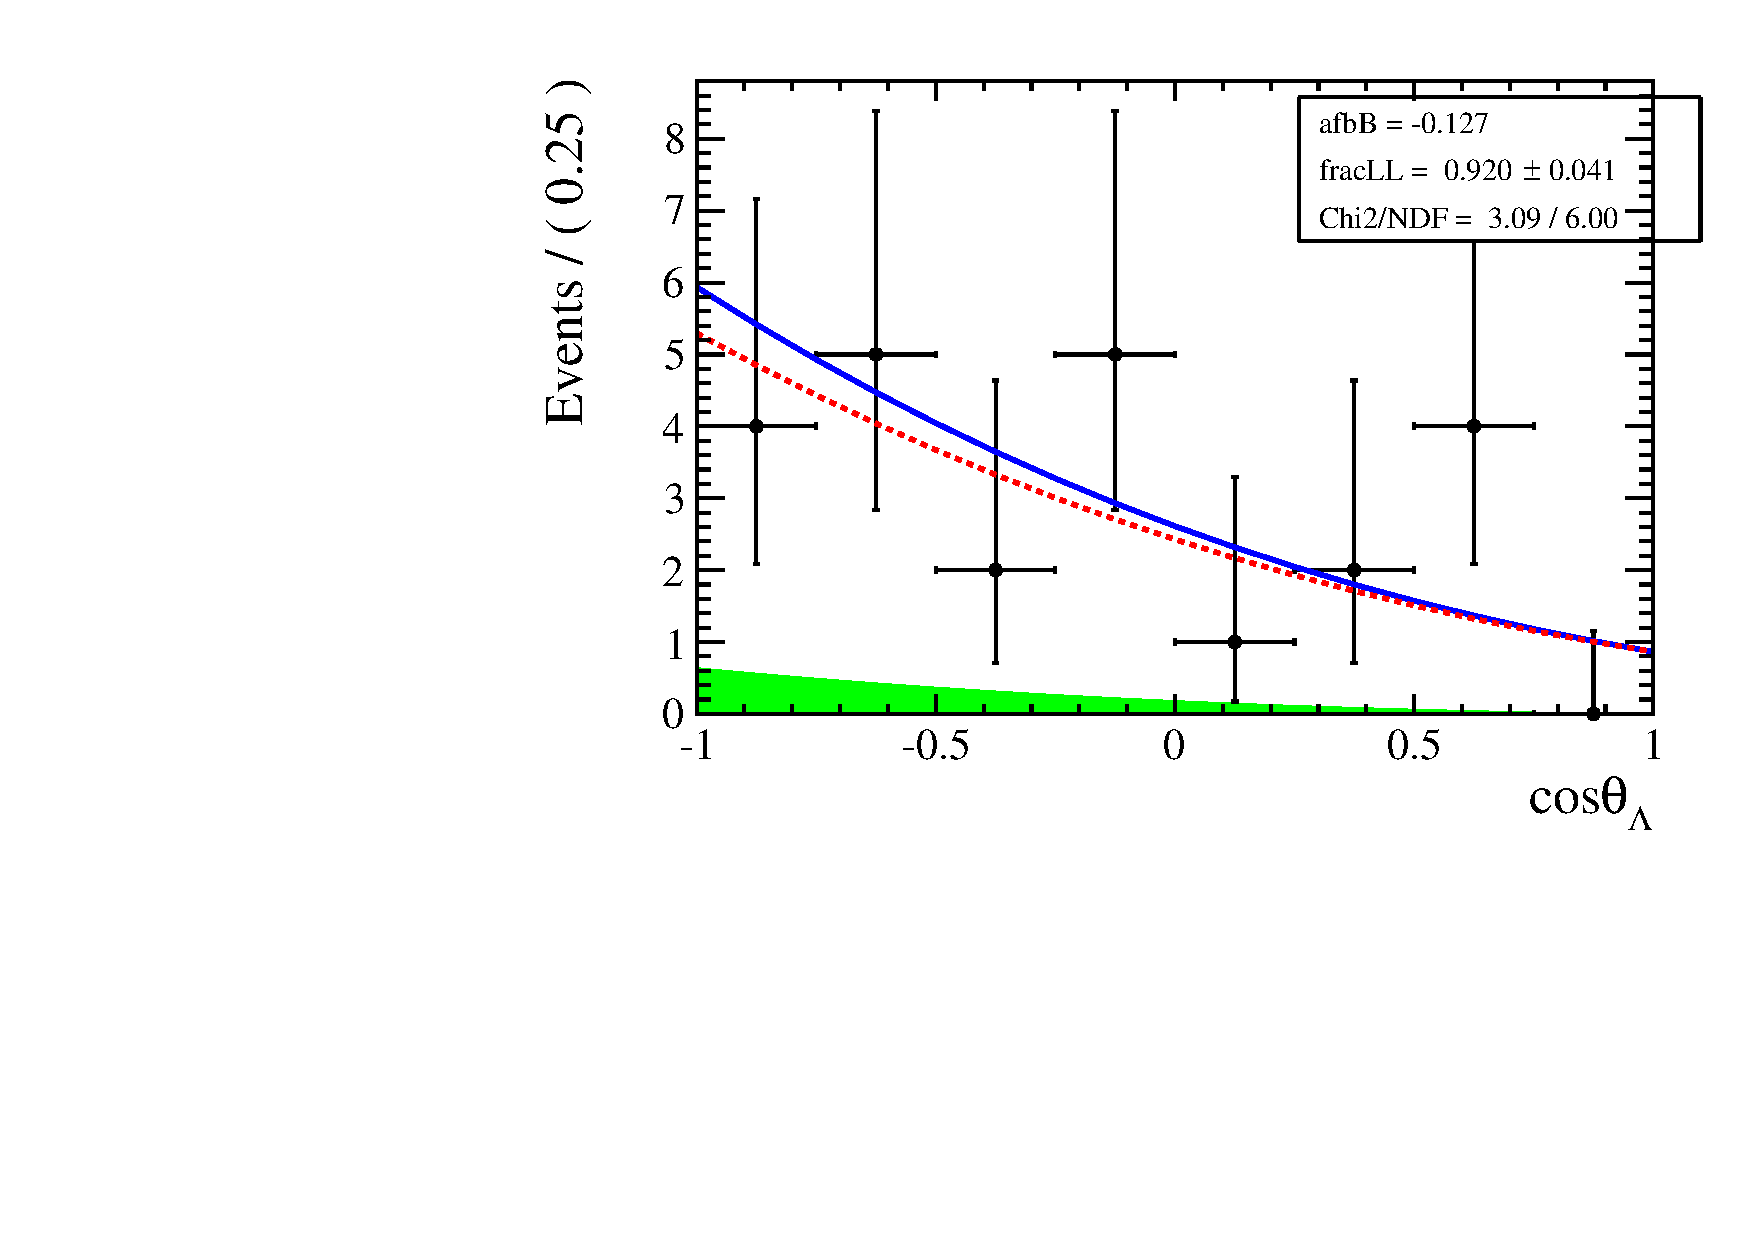
\includegraphics[width=0.40\textwidth]{Lmumu/figs/AfbB_LL_q2_1800_2000.pdf}
\caption{Fitted angular distribution as a function of $\cos\theta_\ell$ (top) and $\cos\theta_\Lambda$ (bottom) for down-down (left) and long-long (right) for events in the $18.0-20.0$GeV^2/c^2$$ \qsq bin.  }
\end{figure}


\begin{figure}[!htb]
\centering
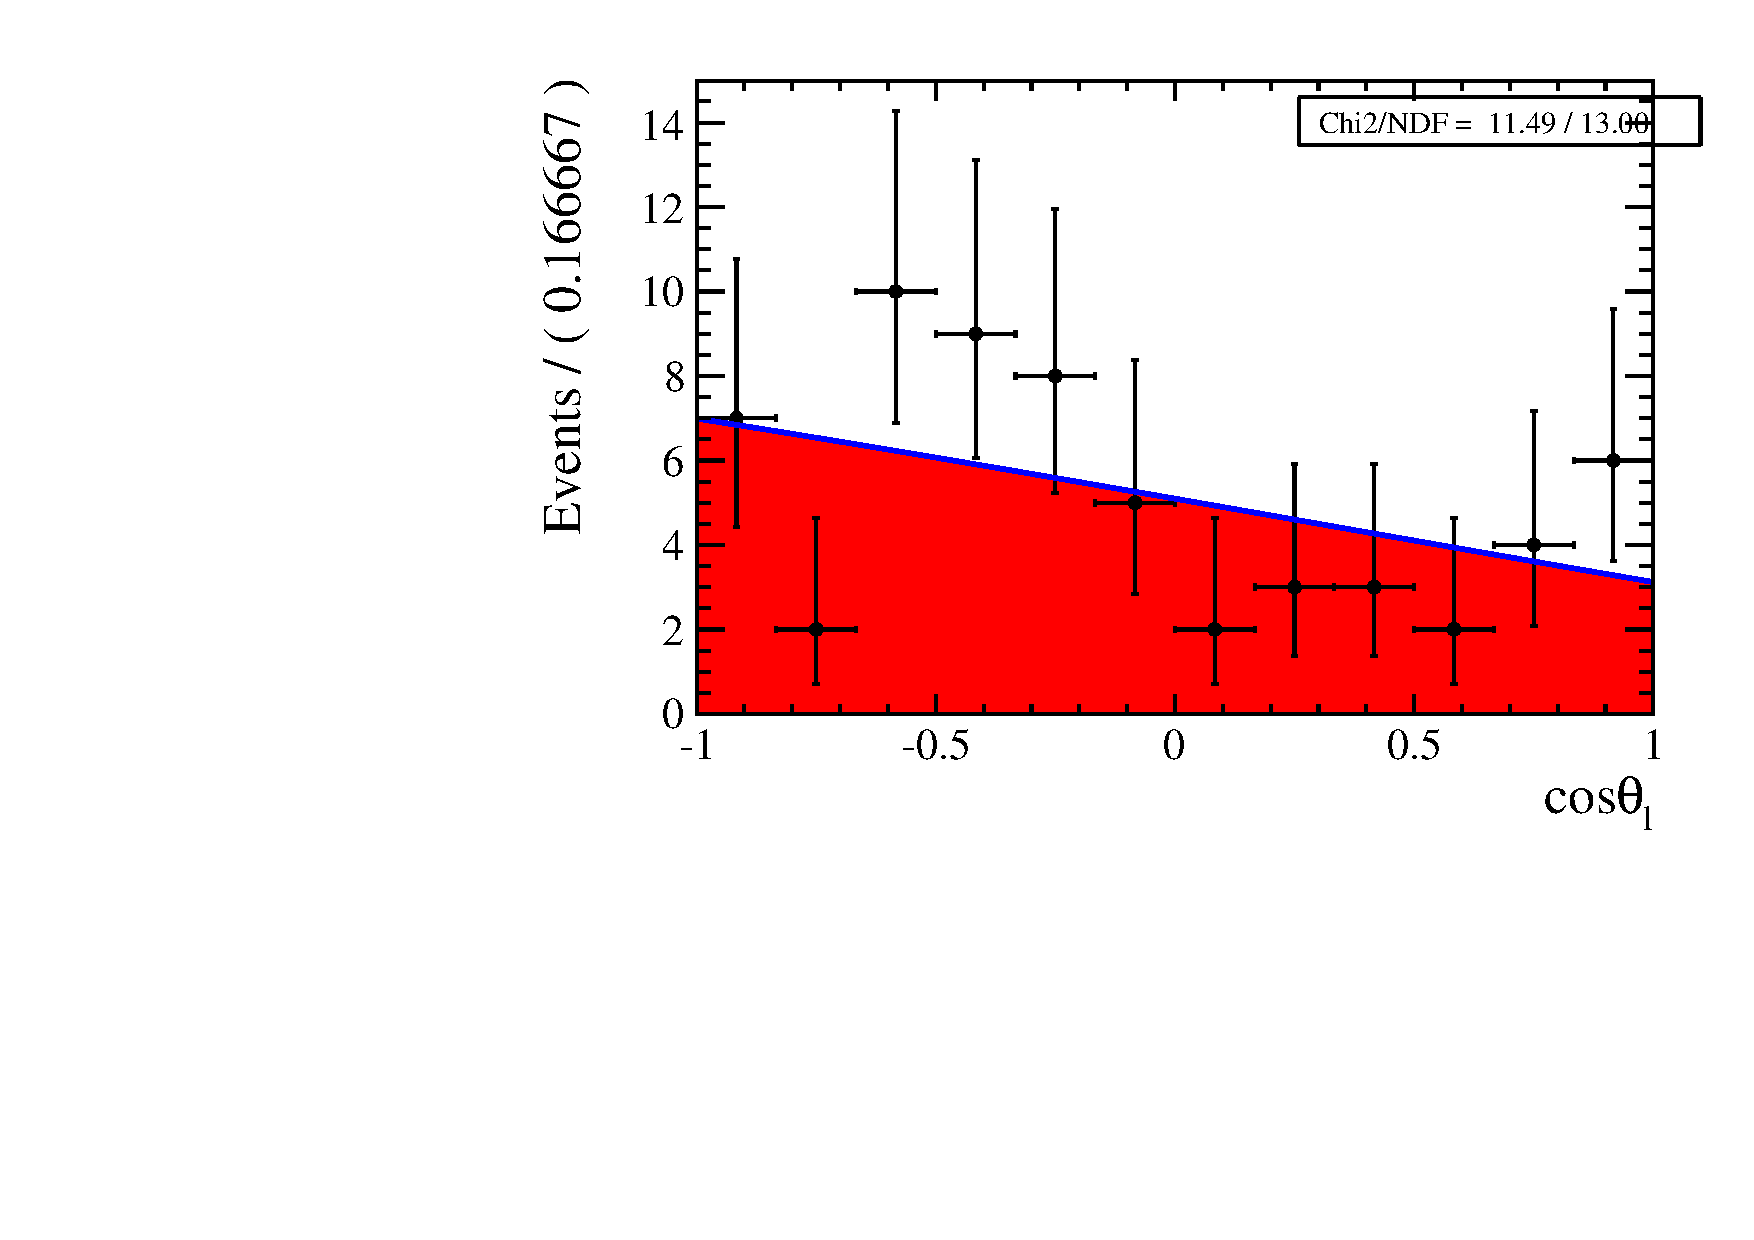
\includegraphics[width=0.40\textwidth]{Lmumu/figs/Side_DD_q2_1800_2000.pdf}
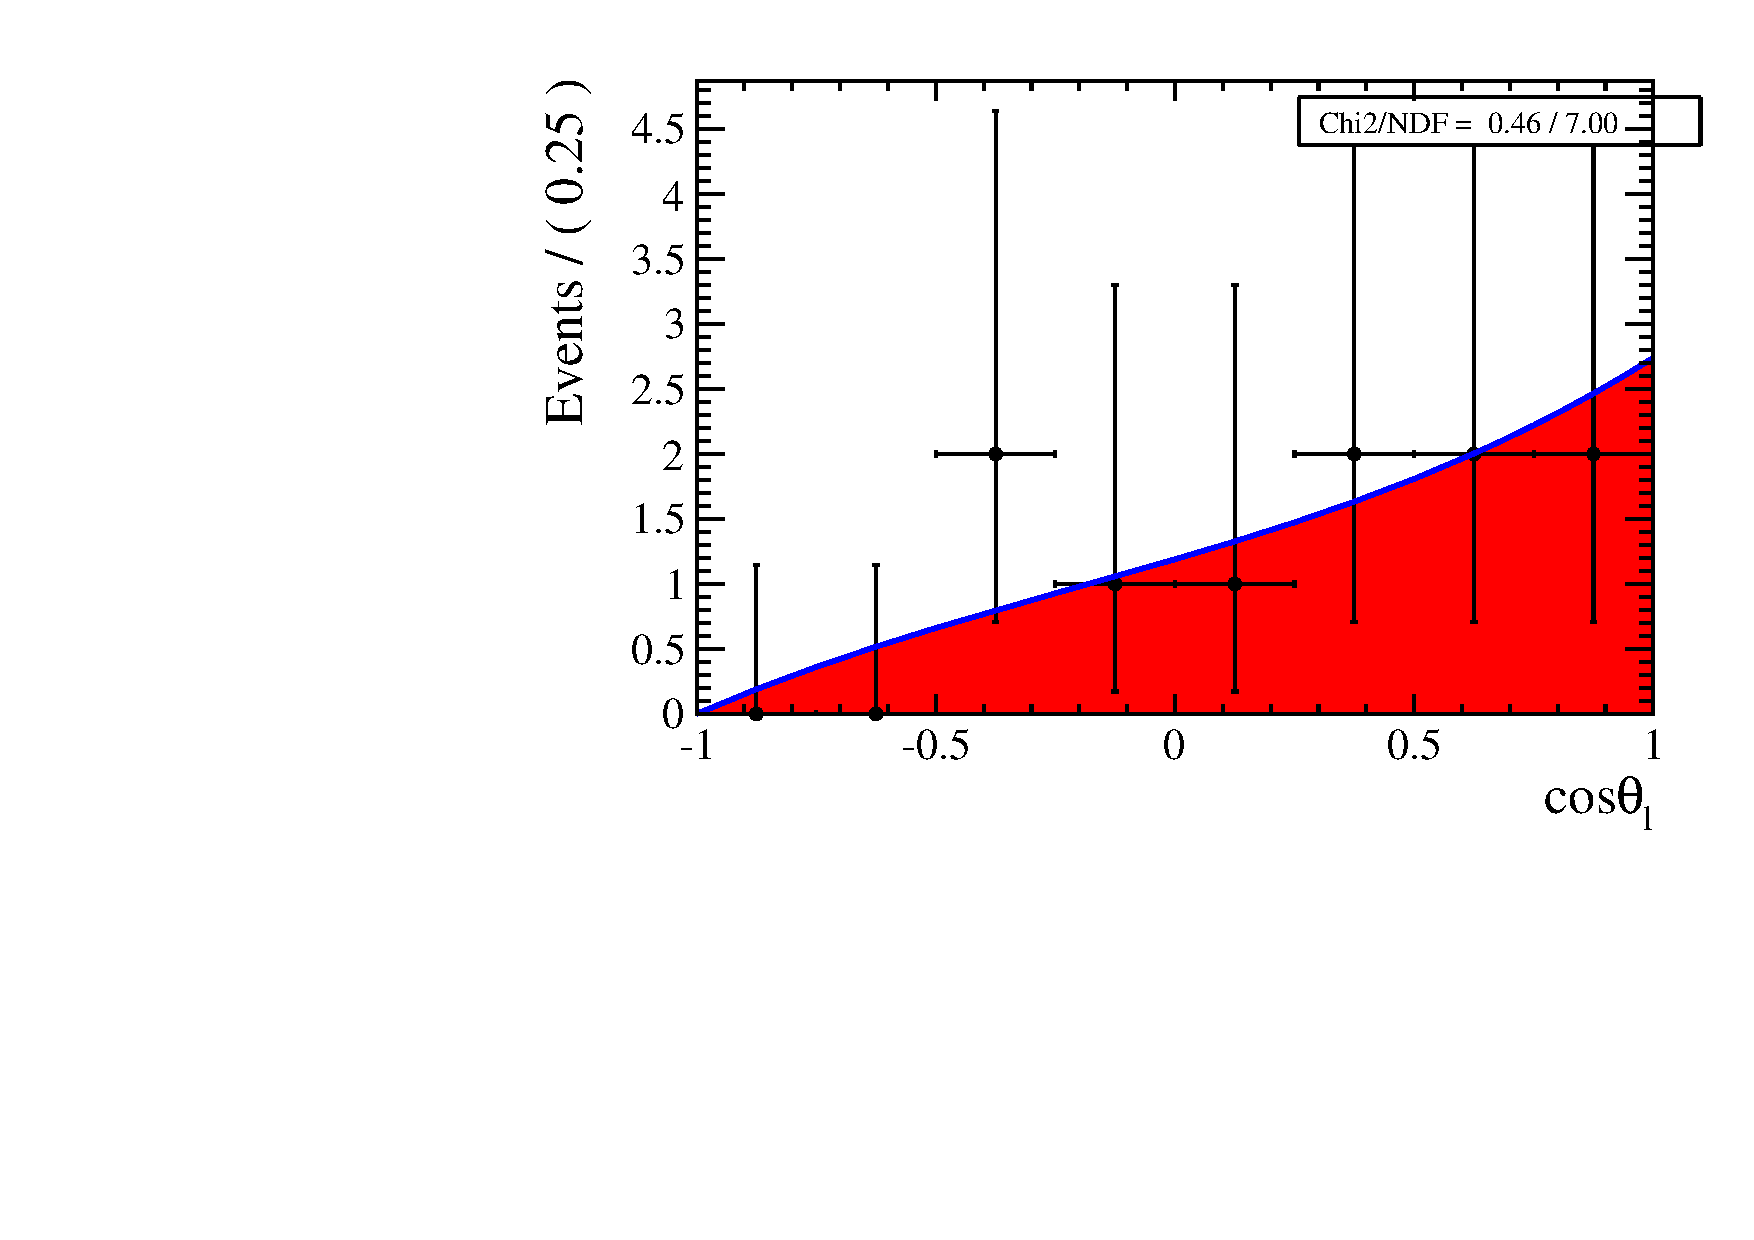
\includegraphics[width=0.40\textwidth]{Lmumu/figs/Side_LL_q2_1800_2000.pdf} \\
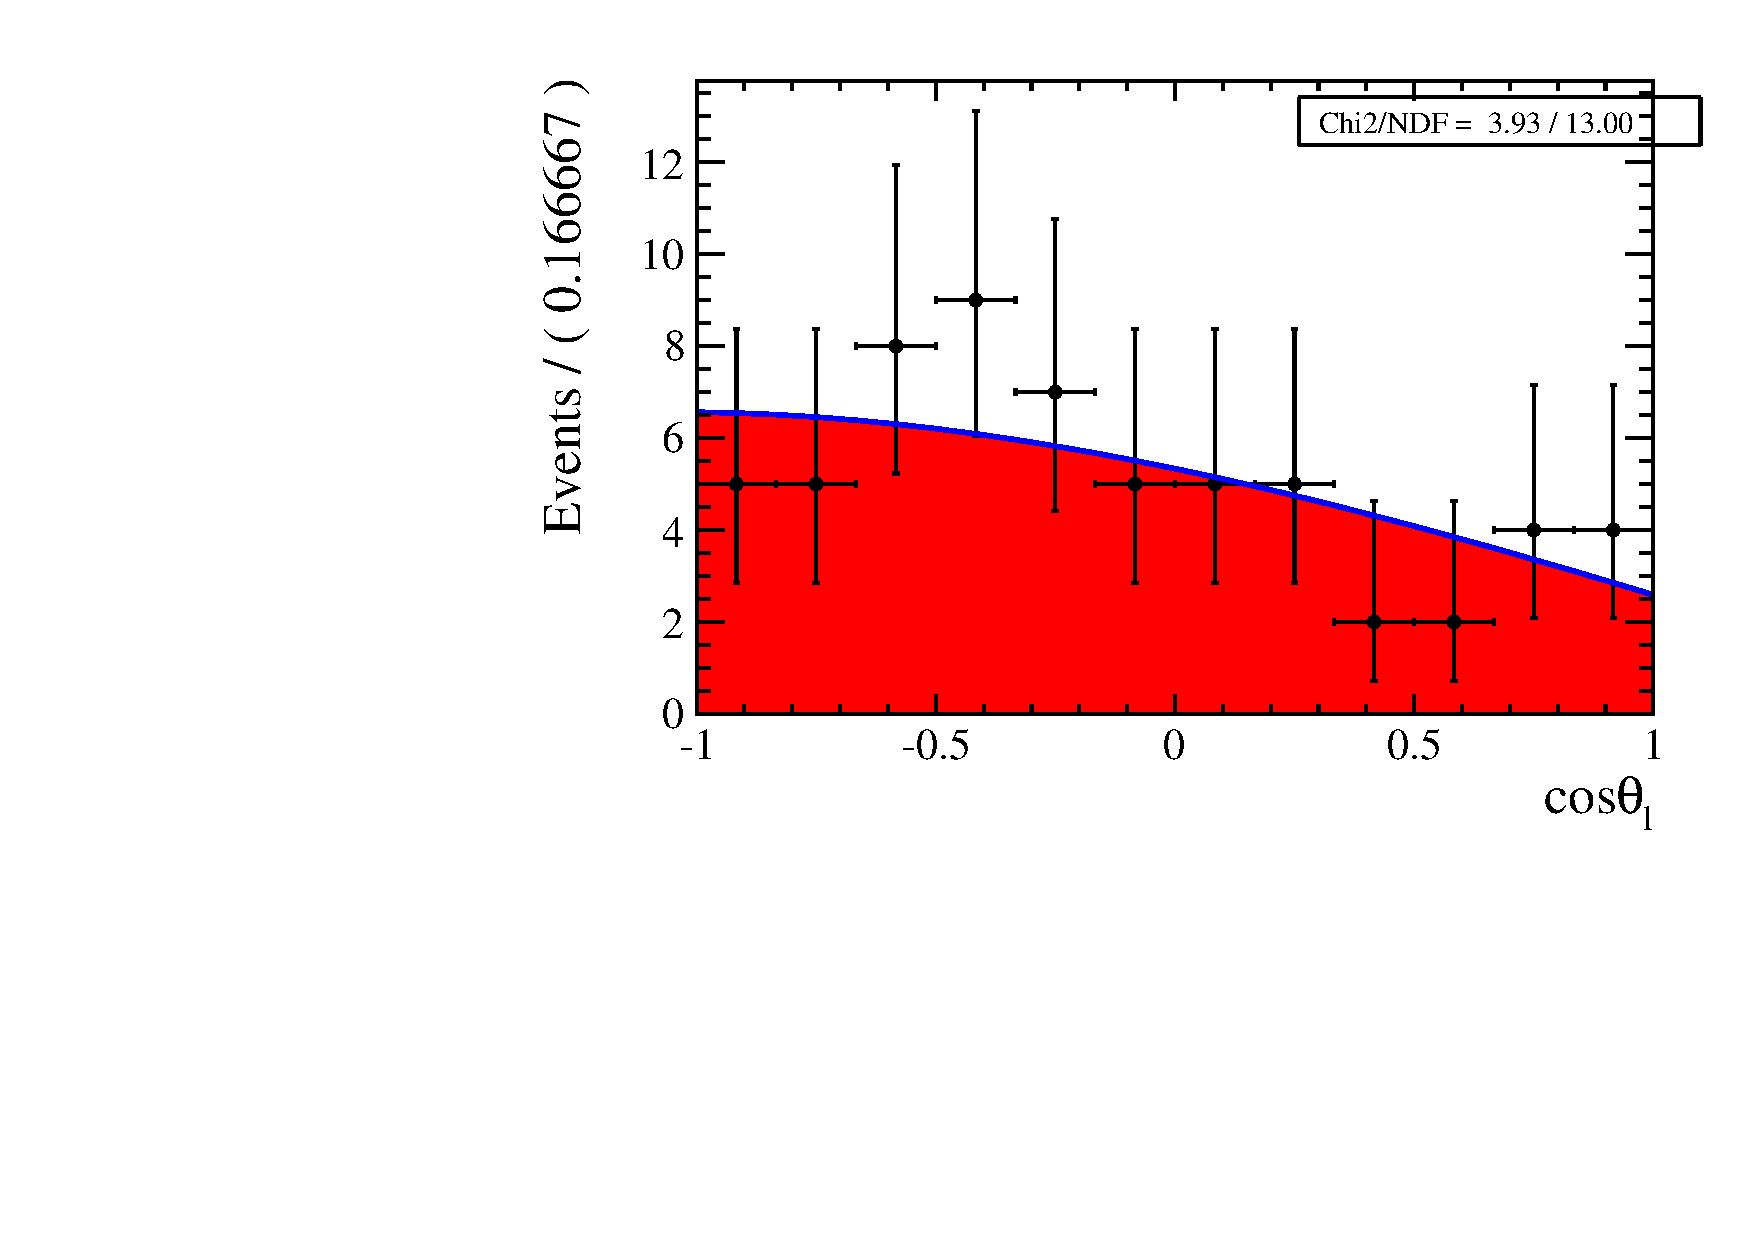
\includegraphics[width=0.40\textwidth]{Lmumu/figs/SideB_DD_q2_1800_2000.pdf}
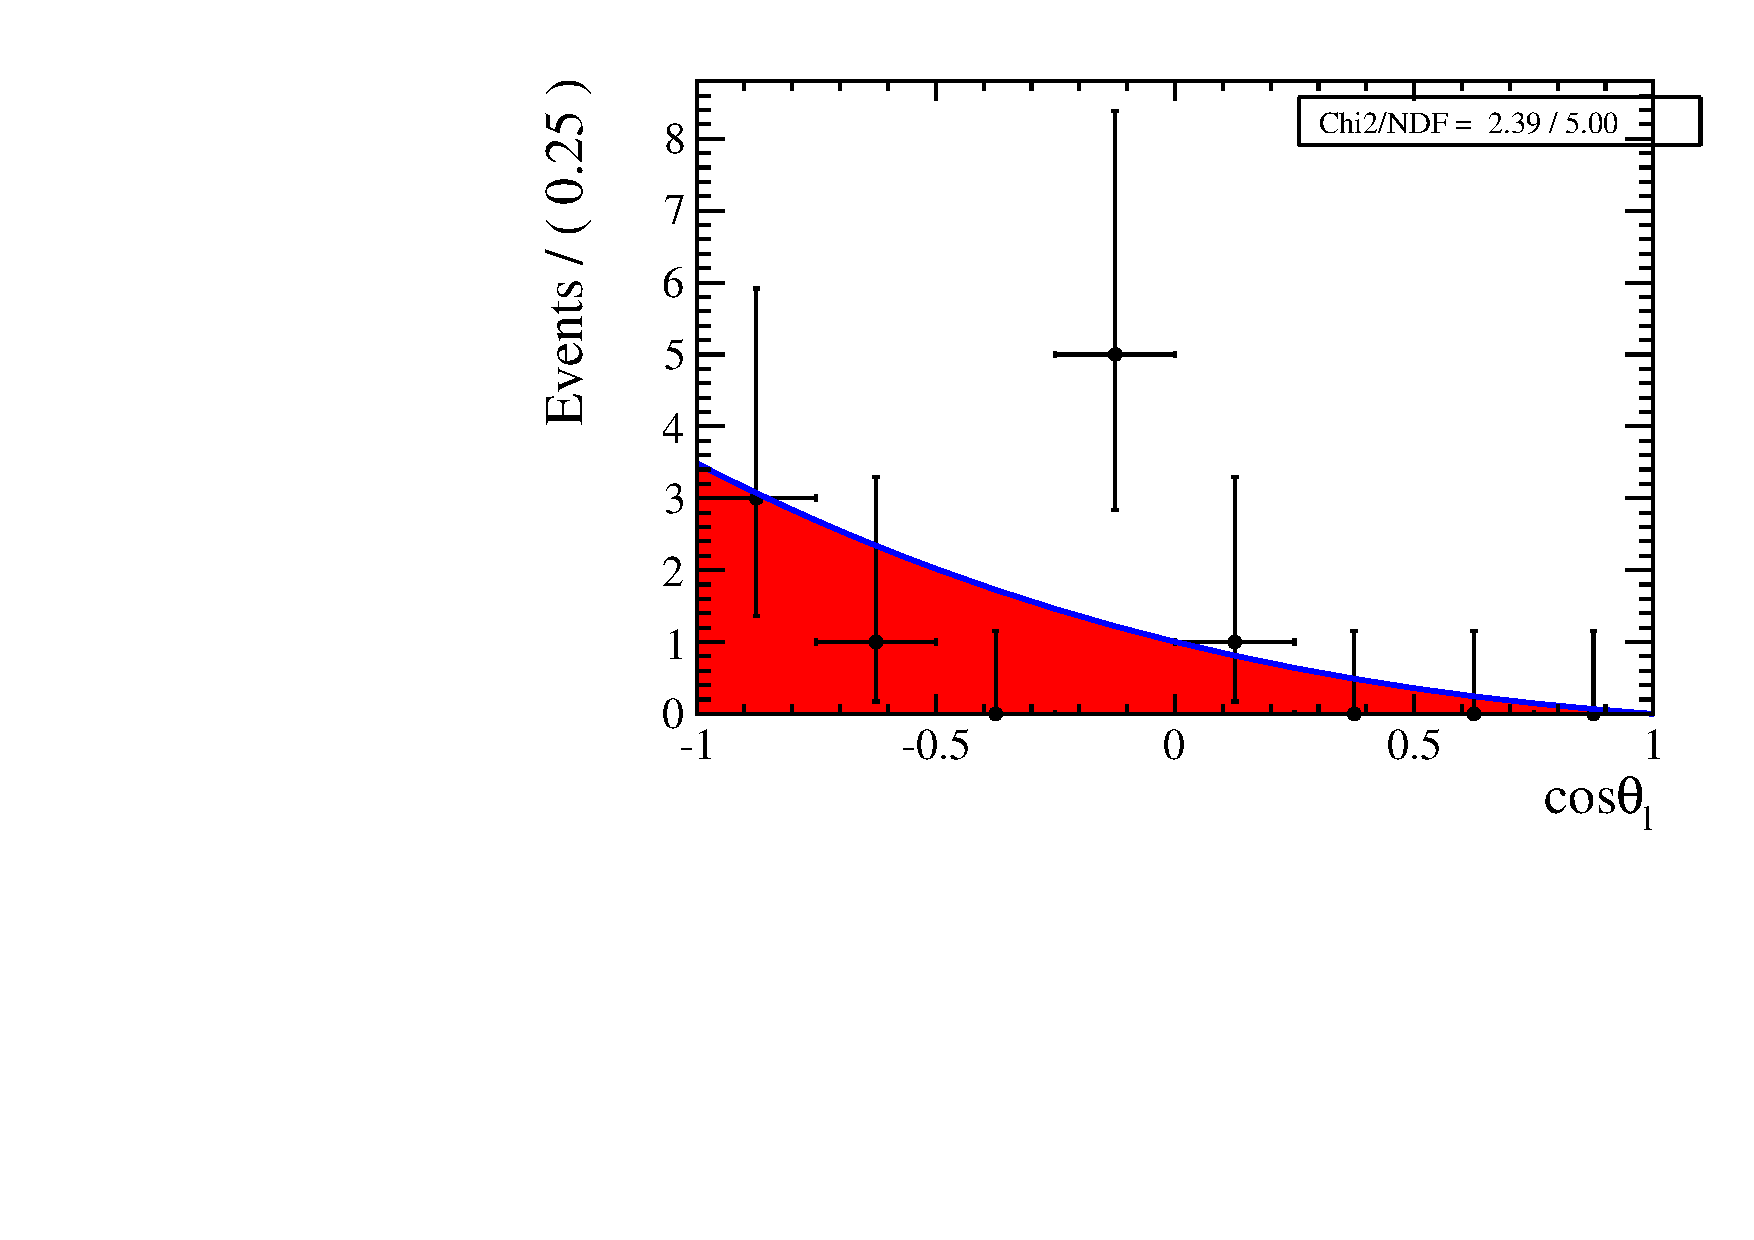
\includegraphics[width=0.40\textwidth]{Lmumu/figs/SideB_LL_q2_1800_2000.pdf}
\caption{Angular distribution in the sideband ($m_{\Lambda\mumu} > 5700 MeV^{2}/c^{2}$) as a function of $\cos\theta_\Lambda$ (top) and $\cos\theta_\Lambda$ (bottom) for down-down (left) and long-long (right) for events in the $18.0-20.0$GeV^2/c^2$$ \qsq bin.  }
\end{figure}







\clearpage
